% This file makes the web version of the blueprint.
% This file can be built locally.

\documentclass{report}

\usepackage[utf8]{inputenc}
\usepackage[english]{babel}
\usepackage{charter}
\usepackage{fancyhdr}
\usepackage{epsf}
\usepackage[bookmarks=true]{hyperref}
\usepackage{amsmath,amsfonts,amsthm,amssymb}
\usepackage{graphicx}
\DeclareGraphicsExtensions{.svg,.png,.jpg}
\usepackage[capitalize]{cleveref}
\usepackage[showmore, dep_graph, project=../../]{blueprint}
\usepackage{tikz-cd}
\usepackage{tikz}

% This file makes the web version of the blueprint.
% This file can be built locally.

\documentclass{report}

\usepackage[utf8]{inputenc}
\usepackage[english]{babel}
\usepackage{charter}
\usepackage{fancyhdr}
\usepackage{epsf}
\usepackage[bookmarks=true]{hyperref}
\usepackage{amsmath,amsfonts,amsthm,amssymb}
\usepackage{graphicx}
\DeclareGraphicsExtensions{.svg,.png,.jpg}
\usepackage[capitalize]{cleveref}
\usepackage[showmore, dep_graph, project=../../]{blueprint}
\usepackage{tikz-cd}
\usepackage{tikz}

% This file makes the web version of the blueprint.
% This file can be built locally.

\documentclass{report}

\usepackage[utf8]{inputenc}
\usepackage[english]{babel}
\usepackage{charter}
\usepackage{fancyhdr}
\usepackage{epsf}
\usepackage[bookmarks=true]{hyperref}
\usepackage{amsmath,amsfonts,amsthm,amssymb}
\usepackage{graphicx}
\DeclareGraphicsExtensions{.svg,.png,.jpg}
\usepackage[capitalize]{cleveref}
\usepackage[showmore, dep_graph, project=../../]{blueprint}
\usepackage{tikz-cd}
\usepackage{tikz}

% This file makes the web version of the blueprint.
% This file can be built locally.

\documentclass{report}

\usepackage[utf8]{inputenc}
\usepackage[english]{babel}
\usepackage{charter}
\usepackage{fancyhdr}
\usepackage{epsf}
\usepackage[bookmarks=true]{hyperref}
\usepackage{amsmath,amsfonts,amsthm,amssymb}
\usepackage{graphicx}
\DeclareGraphicsExtensions{.svg,.png,.jpg}
\usepackage[capitalize]{cleveref}
\usepackage[showmore, dep_graph, project=../../]{blueprint}
\usepackage{tikz-cd}
\usepackage{tikz}

\input{preamble/web}

\github{https://github.com/loganrjmurphy/lean-geo-lib/}
\dochome{https://loganrjmurphy.github.io/lean-geo-lib/docs}

\title{The First Book of Euclid's Elements---Commentary and Lean Formalization}
\author{
    Logan Murphy$^{1}$, Jack Sun$^{1}$, Zhaoyu Li$^{1}$, Anima Anandkumar$^{2}$, Xujie Si$^{1\,\dagger}$, and Kaiyu Yang$^{2\,\dagger}$\\
    $^1$University of Toronto, ~$^2$Caltech\\
    $^\dagger$ Equal advising \\
}

\begin{document}
\maketitle
\input{main}
\end{document}


\github{https://github.com/loganrjmurphy/lean-geo-lib/}
\dochome{https://loganrjmurphy.github.io/lean-geo-lib/docs}

\title{The First Book of Euclid's Elements---Commentary and Lean Formalization}
\author{
    Logan Murphy$^{1}$, Jack Sun$^{1}$, Zhaoyu Li$^{1}$, Anima Anandkumar$^{2}$, Xujie Si$^{1\,\dagger}$, and Kaiyu Yang$^{2\,\dagger}$\\
    $^1$University of Toronto, ~$^2$Caltech\\
    $^\dagger$ Equal advising \\
}

\begin{document}
\maketitle
\input{intro}

\input{definitions}
\input{postulates}
\input{common_notions}

\input{propositions/proposition_1}
\input{propositions/proposition_2}
\input{propositions/proposition_3}
\input{propositions/proposition_4}
\input{propositions/proposition_5}
\input{propositions/proposition_6}
\input{propositions/proposition_7}
\input{propositions/proposition_8}
\input{propositions/proposition_9}
\input{propositions/proposition_10}
\input{propositions/proposition_11}
\input{propositions/proposition_12}
\input{propositions/proposition_13}
\input{propositions/proposition_14}
\input{propositions/proposition_15}
\input{propositions/proposition_16}
\input{propositions/proposition_17}
\input{propositions/proposition_18}
\input{propositions/proposition_19}
\input{propositions/proposition_20}
\input{propositions/proposition_21}
\input{propositions/proposition_22}
\input{propositions/proposition_23}
\input{propositions/proposition_24}
\input{propositions/proposition_25}
\input{propositions/proposition_26}
\input{propositions/proposition_27}
\input{propositions/proposition_28}
\input{propositions/proposition_29}
\input{propositions/proposition_30}
\input{propositions/proposition_31}
\input{propositions/proposition_32}
\input{propositions/proposition_33}
\input{propositions/proposition_34}
\input{propositions/proposition_35}
\input{propositions/proposition_36}
\input{propositions/proposition_37}
\input{propositions/proposition_38}
\input{propositions/proposition_39}
\input{propositions/proposition_40}
\input{propositions/proposition_41}
\input{propositions/proposition_42}
\input{propositions/proposition_43}
\input{propositions/proposition_44}
\input{propositions/proposition_45}
\input{propositions/proposition_46}
\input{propositions/proposition_47}
\input{propositions/proposition_48}

\end{document}


\github{https://github.com/loganrjmurphy/lean-geo-lib/}
\dochome{https://loganrjmurphy.github.io/lean-geo-lib/docs}

\title{The First Book of Euclid's Elements---Commentary and Lean Formalization}
\author{
    Logan Murphy$^{1}$, Jack Sun$^{1}$, Zhaoyu Li$^{1}$, Anima Anandkumar$^{2}$, Xujie Si$^{1\,\dagger}$, and Kaiyu Yang$^{2\,\dagger}$\\
    $^1$University of Toronto, ~$^2$Caltech\\
    $^\dagger$ Equal advising \\
}

\begin{document}
\maketitle
\chapter{Introduction}

\chapter{Definitions}

\begin{enumerate}
    \item \label{def:1} A point is that of which there is no part.
    \item \label{def:2} And a line is a length without breadth.
    \item \label{def:3} And the extremities of a line are points.
    \item \label{def:4} A straight-line is (any) one which lies evenly with points on itself.
    \item \label{def:5} And a surface is that which has length and breadth only.
    \item \label{def:6} And the extremities of a surface are lines.
    \item \label{def:7} A plane surface is (any) one which lies evenly with the straight-lines on itself.
    \item \label{def:8} And a plane angle is the inclination of the lines to one another, when two lines in a plane meet one another, and are not lying in a straight-line.
    \item \label{def:9} And when the lines containing the angle are straight then the angle is called rectilinear.
    \item \label{def:10} And when a straight-line stood upon (another) straight-line makes adjacent angles (which are) equal to one another, each of the equal angles is a right-angle, and the former straight-line is called a perpendicular to that upon which it stands.
    \item \label{def:11} An obtuse angle is one greater than a right-angle.
    \item \label{def:12} And an acute angle (is) one less than a right-angle.
    \item \label{def:13} A boundary is that which is the extremity of something.
    \item \label{def:14} A figure is that which is contained by some boundary or boundaries.
    \item \label{def:15} A circle is a plane figure contained by a single line [which is called a circumference], (such that) all of the straight-lines radiating towards [the circumference] from one point amongst those lying inside the figure are equal to one another.
    \item \label{def:16} And the point is called the center of the circle.
    \item \label{def:17} And a diameter of the circle is any straight-line, being drawn through the center, and terminated in each direction by the circumference of the circle. (And) any such (straight-line) also cuts the circle in half.
    \item \label{def:18} And a semi-circle is the figure contained by the diameter and the circumference cuts off by it. And the center of the semi-circle is the same (point) as (the center of) the circle.
    \item \label{def:19} Rectilinear figures are those (figures) contained by straight-lines: trilateral figures being those contained by three straight-lines, quadrilateral by four, and multilateral by more than four.
    \item \label{def:20} And of the trilateral figures: an equilateral triangle is that having three equal sides, an isosceles (triangle) that having only two equal sides, and a scalene (triangle) that having three unequal sides.
    \item \label{def:21} And further of the trilateral figures: a right-angled triangle is that having a right-angle, an obtuse-angled (triangle) that having an obtuse angle, and an acute-angled (triangle) that having three acute angles.
    \item \label{def:22} And of the quadrilateral figures: a square is that which is right-angled and equilateral, a rectangle that which is right-angled but not equilateral, a rhombus that which is equilateral but not right-angled, and a rhomboid that having opposite sides and angles equal to one another which is neither right-angled nor equilateral. And let quadrilateral figures besides these be called trapezia.
    \item \label{def:23} Parallel lines are straight-lines which, being in the same plane, and being produced to infinity in each direction, meet with one another in neither (of these directions).
\end{enumerate}
\chapter{Postulates}

\begin{enumerate}
    \item \label{post:1} Let it have been postulated to draw a straight-line from any point to any point.
    \item \label{post:2} And to produce a finite straight-line continuously in a straight-line.
    \item \label{post:3} And to draw a circle with any center and radius.
    \item \label{post:4} And that all right-angles are equal to one another.
    \item \label{post:5} And that if a straight-line falling across two (other) straight-lines makes internal angles on the same side (of itself whose sum is) less than two right-angles, then the two (other) straight-lines, being produced to infinity, meet on that side (of the original straight-line) that the (sum of the internal angles) is less than two right-angles (and do not meet on the other side).
\end{enumerate}

\chapter{Common Notions}

\begin{enumerate}
    \item \label{cn:1} Things equal to the same thing are also equal to one another.
    \item \label{cn:2} And if equal things are added to equal things then the wholes are equal.
    \item \label{cn:3} And if equal things are subtracted from equal things then the remainders are equal.
    \item \label{cn:4} And things coinciding with one another are equal to one another.
    \item \label{cn:5} And the whole [is] greater than the part.
\end{enumerate}



\chapter*{Proposition 1}
\label{prop:1}

\begin{figure*}[ht]
    \begin{center}
    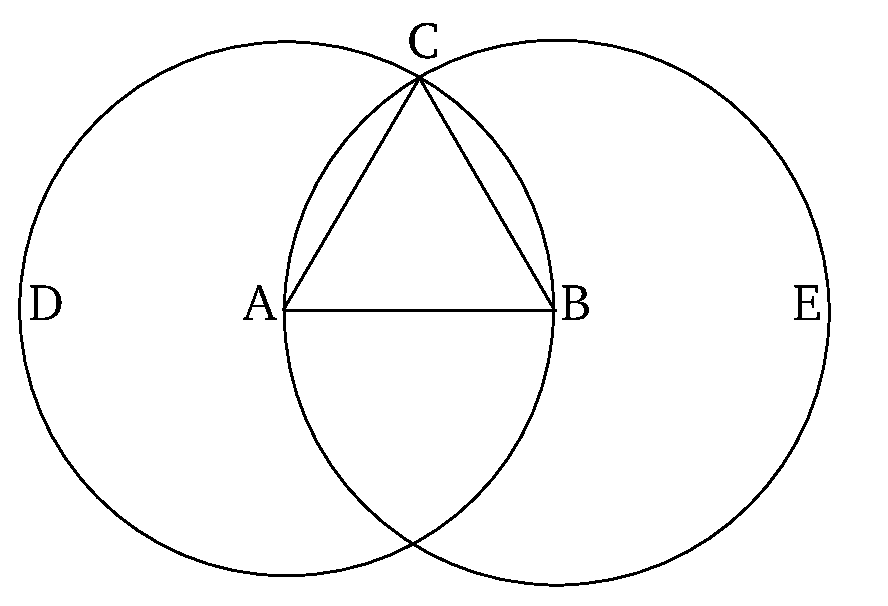
\includegraphics[width=0.5\linewidth]{figures/fig01e.eps}
    \label{fig:prop_1}
    \end{center}
\end{figure*}

To construct an equilateral triangle on a given finite straight-line.

Let $AB$ be the given finite straight-line. 

So it is required to construct an equilateral triangle on the straight-line $AB$.

Let the circle $BCD$ with center $A$ and radius $AB$ have been drawn [Post.~\ref{post:3}], and again let the circle $ACE$ with center $B$ and radius $BA$ have been drawn [Post.~\ref{post:3}].
And let the straight-lines $CA$ and $CB$ have been joined from the point $C$, where the circles cut one another, to the points $A$ and $B$ (respectively) [Post.~\ref{post:1}].

And since the point $A$ is the center of the circle $CDB$, $AC$ is equal to $AB$ [Def.~\ref{def:5}]. Again,
since the point $B$ is the center of the circle $CAE$, $BC$ is equal to $BA$ [Def.~\ref{def:5}]. But $CA$ 
was also shown (to be) equal to $AB$. Thus, $CA$ and $CB$ are each equal to $AB$. But things equal to the same thing are also equal to one another [C.N.~\ref{cn:1}]. Thus, $CA$ is also equal to $CB$. Thus, the three (straight-lines) $CA$, $AB$, and $BC$ are equal to one another.

Thus, the triangle $ABC$ is equilateral, and has been constructed on the
given finite straight-line $AB$. (Which is) the very thing it was required to do.

\section*{Commentary}

\begin{proposition}\label{proposition_1}\lean{Elements.Book1.proposition_1}\leanok
    Given two disctinct points $A$ and $B$ on a line $AB$, there must be a point $C$, s.t. $\triangle~ABC$ is an equilateral triangle.
\end{proposition}
\begin{proof}
    \leanok
    See the original proof by Euclid.
\end{proof}

Euclid omitted the fact that point $C$ can be constructed on either side of $AB$, which is required for proving latter propositions.
We state and prove this fact as Prop.~\ref{proposition_1'}.

\begin{proposition}\label{proposition_1'}\lean{Elements.Book1.proposition_1'}\leanok
    $A$ and $B$ are two disctinct points on a line $AB$. $X$ is a point not on $AB$. Then there must be a point $C$ on the opposite side of $AB$ from $X$, s.t. $\triangle~ABC$ is an equilateral triangle.
\end{proposition}
\begin{proof}
    \leanok
    Similar to Euclid's proof but note that the point $C$ can be constructed on either side.
\end{proof}
\chapter*{Proposition 2}
\label{prop:2}

\begin{figure*}[ht]
    \begin{center}
    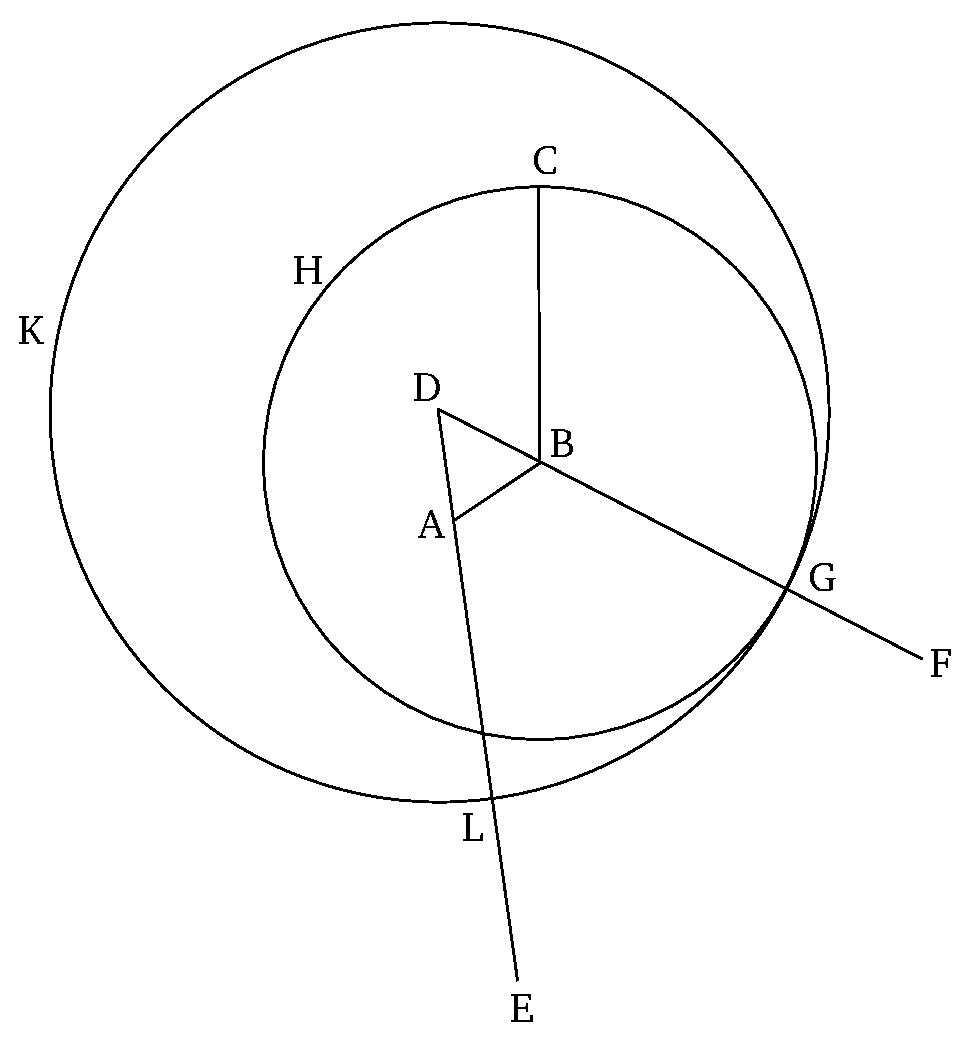
\includegraphics[width=0.5\linewidth]{figures/fig02e.eps}
    \label{fig:prop_2}
    \end{center}
\end{figure*}

To place a straight-line equal to a given straight-line at a given point (as an extremity).

Let $A$ be the given point, and $BC$ the given straight-line. So  it is required to
place a straight-line at point $A$ equal to the given straight-line $BC$.

For let the straight-line $AB$ have been joined from point $A$ to point $B$ [Post.~\ref{post:1}], and let the
equilateral triangle $DAB$ have been been constructed upon it [Prop.~1.1].  And let the
straight-lines $AE$ and $BF$ have been produced in a straight-line with $DA$ and $DB$  (respectively) [Post.~\ref{post:2}].
And let the circle $CGH$ with center $B$ and radius $BC$ have been drawn
[Post.~\ref{post:3}], and again let the circle $GKL$ with center $D$ and radius $DG$ have been drawn [Post.~\ref{post:3}].

Therefore, since the point $B$ is the center of (the circle) $CGH$, $BC$ is equal to 
$BG$ [Def.~\ref{def:5}]. Again, since the point $D$ is the center of the circle $GKL$, $DL$ is equal to $DG$ [Def.~\ref{def:5}]. And within these,  $DA$ is equal to $DB$. Thus, the remainder $AL$ is equal to the remainder $BG$ [C.N.~\ref{cn:3}]. But $BC$ was also shown (to be)  equal to $BG$. Thus,  $AL$
and $BC$ are each equal to $BG$. But things equal to the same thing are also equal to one another [C.N.~\ref{cn:1}]. Thus, $AL$ is also equal to $BC$.

Thus, the straight-line $AL$, equal to the given straight-line $BC$,
has been placed at the given point $A$. (Which is) the very thing it was required to do.

\section*{Commentary}

\begin{proposition}\label{proposition_2}\lean{Elements.Book1.proposition_2}\leanok
    $B$ and $C$ are two distinct points on a line $BC$. $A$ is a point different from $B$. There must be a point $L$, s.t. $|AL| = |BC|$.
\end{proposition}
\begin{proof}
    \uses{proposition_1}\leanok
    See the original proof by Euclid.
\end{proof}

Euclid omitted the degenerated case where $A$ is the same as $B$.

\begin{proposition}\label{proposition_2'}\lean{Elements.Book1.proposition_2'}\leanok
    $B$ and $C$ are two distinct points on a line $BC$. For any point $A$, there must be a point $L$, s.t. $|AL| = |BC|$.
\end{proposition}
\begin{proof}
    \uses{proposition_1,proposition_2}
    \leanok
    When $A = B$, we can just take $L = C$.
    When $A \neq B$, we apply Prop.~\ref{proposition_2}.
\end{proof}
\chapter*{Proposition 3}
\label{prop:3}

\begin{figure*}[ht]
    \begin{center}
    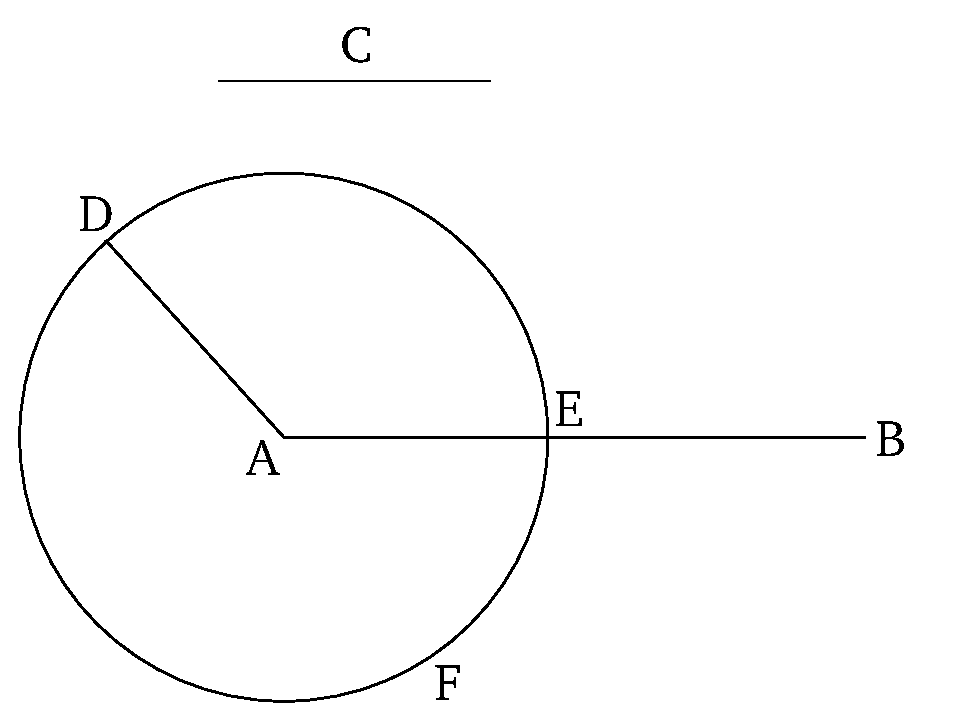
\includegraphics[width=0.5\linewidth]{figures/fig03e.eps}
    \label{fig:prop_3}
    \end{center}
\end{figure*}

For two given unequal straight-lines, to cut off from the greater a straight-line
equal to the lesser.

Let $AB$ and $C$ be the two given unequal straight-lines, of which let the greater be $AB$. So it is required to cut off a straight-line equal to the lesser $C$ from the greater $AB$.

Let the line $AD$, equal to the straight-line $C$, have been placed at  point $A$ [Prop.~1.2]. And let
the circle $DEF$ have been drawn with center $A$ and radius $AD$ [Post.~\ref{post:3}].

And since  point $A$ is the center of  circle $DEF$, $AE$ is equal to $AD$ [Def.~\ref{def:5}]. But,
$C$ is also equal to $AD$. Thus, $AE$ and $C$ are each equal to $AD$. So $AE$
is also equal to $C$ [C.N.~\ref{cn:1}].

Thus, for two given unequal straight-lines, $AB$ and $C$, the (straight-line) $AE$, equal to
the lesser $C$, has been cut off from the greater $AB$. (Which is) the very thing it was required to do.

\section*{Commentary}

\begin{proposition}\label{proposition_3}\lean{Elements.Book1.proposition_3}\leanok
   $A$ and $B$ are two distinct points on a line $AB$. $C_0$ and $C_1$ are two distinct points on a line $C$. $A \neq C_0$, and $|AB| > |C_0C_1|$. There must be a point $E$ between $A$ and $B$, s.t., $|AE| = |C_0C_1|$
\end{proposition}
\begin{proof}
    \uses{proposition_3}\leanok
    See the original proof by Euclid.
\end{proof}

\chapter*{Proposition 4}
\label{prop:4}


\begin{figure*}[ht]
    \begin{center}
    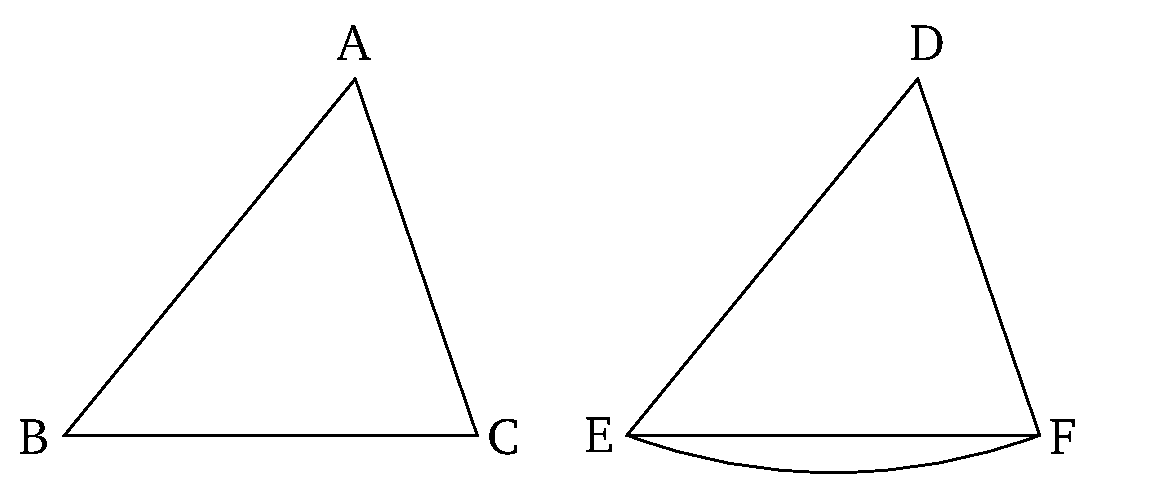
\includegraphics[width=0.5\linewidth]{figures/fig04e.eps}
    \label{fig:prop_4}
    \end{center}
\end{figure*}

If two triangles have two sides equal to two sides, respectively, and have the
angle(s) enclosed by the equal straight-lines equal, then
they will also have the base equal to the base, and the triangle will be equal
to the triangle, and the remaining angles subtended by the equal sides will be equal to the corresponding remaining angles.

Let $ABC$ and $DEF$ be  two triangles having the two sides $AB$ and $AC$ equal to the two sides $DE$ and $DF$, respectively. (That is) $AB$ to $DE$, and $AC$ to $DF$. And (let) the angle $BAC$ (be) equal to the angle $EDF$. I say that the base $BC$ is also equal to the base
$EF$, and triangle $ABC$ will be equal to triangle $DEF$, and the remaining angles
subtended by the equal sides will be equal to the corresponding remaining angles. (That is) $ABC$ to $DEF$, and $ACB$ to
$DFE$.

For if triangle $ABC$ is applied to triangle $DEF$, the point $A$ being placed
on the point $D$, and the straight-line $AB$ on $DE$, then the point $B$ will also coincide with $E$, on account of $AB$ being equal to $DE$. So (because of) $AB$ coinciding with $DE$, the straight-line $AC$ will also coincide with $DF$, on account of the angle $BAC$ being equal to $EDF$. So the point $C$ will also coincide with the
point $F$,  again on account of $AC$ being equal to $DF$.  But,  point $B$  certainly also coincided with point $E$, so that the base $BC$ will coincide with the base $EF$.
For if $B$ coincides with $E$, and $C$ with $F$, and the base $BC$ does not coincide with $EF$, then two straight-lines will encompass an area. The very thing is impossible [Post.~\ref{post:1}]. Thus, the base $BC$ will coincide with $EF$, and will be equal to it [C.N.~\ref{cn:4}]. So  the whole triangle $ABC$ will coincide with the whole triangle $DEF$, and will be equal to it [C.N.~\ref{cn:4}]. And the remaining angles will coincide with the remaining angles, and  will be equal to them [C.N.~\ref{cn:4}]. (That is) $ABC$ to $DEF$, and $ACB$
to $DFE$ [C.N.~\ref{cn:4}].

Thus, if two triangles have two  sides equal to two sides, respectively, and have the
angle(s) enclosed by the equal straight-line equal, then
they will also have the base equal to the base, and the triangle will be equal
to the triangle,  and
the remaining angles subtended by the equal sides will be equal to the
corresponding remaining angles. (Which is) the very thing it was required to show.


\section*{Commentary}

\begin{proposition}\label{proposition_4}\lean{Elements.Book1.proposition_4}\leanok
    $\triangle~ABC$ and $\triangle~DEF$ are two triangles with $|AB| = |DE|$, $|AC| = |DF|$, and $\angle~BAC = \angle~EDF$. Then, $\triangle~ABC$ and $\triangle~DEF$ must be congruent. That is, $|BC| = |EF|$, $\angle~ABC = \angle~DEF$, and $\angle~ACB = \angle~DFE$.
\end{proposition}
\begin{proof}
    \leanok
    See the original proof by Euclid.
\end{proof}

\chapter*{Proposition 5}
\label{prop:5}

\begin{figure*}[ht]
    \begin{center}
    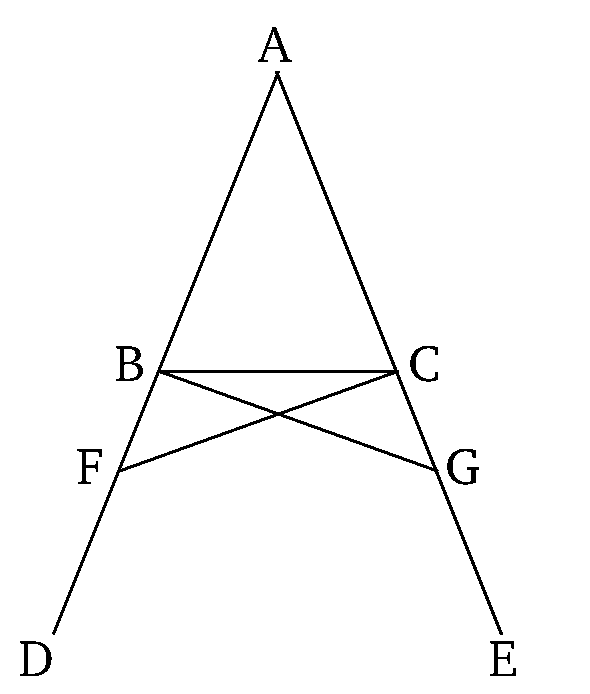
\includegraphics[width=0.5\linewidth]{figures/fig05e.eps}
    \label{fig:prop_5}
    \end{center}
\end{figure*}

For isosceles triangles, the angles at the base are equal to one another, and if
the equal sides are produced then the angles under the base will be equal to one another.

Let $ABC$ be an isosceles triangle having the side $AB$ equal to the side $AC$, and let the straight-lines $BD$ and $CE$ have been produced in a straight-line
with $AB$ and $AC$ (respectively) [Post.~\ref{post:2}]. I say that the angle $ABC$ is equal to $ACB$, and (angle) $CBD$  to $BCE$.

For let the point $F$ have been taken at random on  $BD$, and let $AG$
have been cut off from the greater $AE$, equal to the lesser $AF$ [Prop.~1.3]. Also, let
the straight-lines $FC$ and $GB$ have been joined [Post.~\ref{post:1}].

In fact, since $AF$ is equal to $AG$, and $AB$ to $AC$, the two (straight-lines) $FA$, $AC$ are
equal to the two (straight-lines) $GA$, $AB$, respectively. They also encompass a
common angle, $FAG$. Thus, the base $FC$ is equal to the base $GB$, and the
triangle $AFC$ will be equal to the triangle $AGB$, and the remaining angles
subtendend by the equal sides will
be equal to the corresponding  remaining angles [Prop.~1.4].  (That is) $ACF$ to $ABG$, and $AFC$ to $AGB$. And since the whole of $AF$ is
equal to the whole of $AG$, within which $AB$ is equal to $AC$, the remainder
$BF$ is thus equal to the remainder $CG$ [C.N.~\ref{cn:3}]. But $FC$ was also shown (to be) equal to $GB$. So
the two (straight-lines) $BF$, $FC$ are equal to the two (straight-lines) $CG$, $GB$, respectively,
and the angle $BFC$ (is) equal to the angle $CGB$, and the base $BC$ is common to
them. Thus, the triangle $BFC$ will be equal to the triangle $CGB$, and
the remaining angles subtended by the equal sides will be equal to the corresponding remaining angles [Prop.~1.4]. Thus, $FBC$ is equal to $GCB$, and $BCF$ to
$CBG$. Therefore, since the whole angle $ABG$ was shown (to be) equal to the
whole angle $ACF$, within which $CBG$ is equal to $BCF$, the remainder $ABC$
is thus equal to the remainder $ACB$ [C.N.~\ref{cn:3}]. And they are at the base of triangle
$ABC$. And $FBC$ was also shown (to be) equal to $GCB$. And they are under
the base.

Thus, for isosceles triangles, the angles at the base are equal to one another, and if
the equal sides are produced then the angles under the base will be equal to one another. (Which is) the very thing it was required to show.



\section*{Commentary}

\begin{proposition}\label{proposition_5}\lean{Elements.Book1.proposition_5}\leanok
    $|AB| = |AC|$ in $\triangle~ABC$. $AB$ is extended to $D$, and $AC$ is extended to $E$. Then, $\angle~ABC = \angle~ACB$ and $\angle~CBD = \angle~BCE$.
\end{proposition}
\begin{proof}
    \uses{proposition_3,proposition_4}\leanok
    See the original proof by Euclid.
\end{proof}

Euclid often use the following restricted version of Prop.~\ref{proposition_5} in later proofs.

\begin{proposition}\label{proposition_5'}\lean{Elements.Book1.proposition_5'}\leanok
    For $\triangle~ABC$, if $|AB| = |AC|$, then $\angle~ABC = \angle~ACB$.
\end{proposition}
\begin{proof}
    \uses{proposition_3,proposition_4,proposition_5}\leanok
    Extend $AB$ to $D$ and $AC$ to $E$. Then, $\angle~ABC = \angle~ACB$ by Prop.~\ref{proposition_5}.
\end{proof}
\chapter*{Proposition 6}
\label{prop:6}

\begin{figure*}[ht]
    \begin{center}
    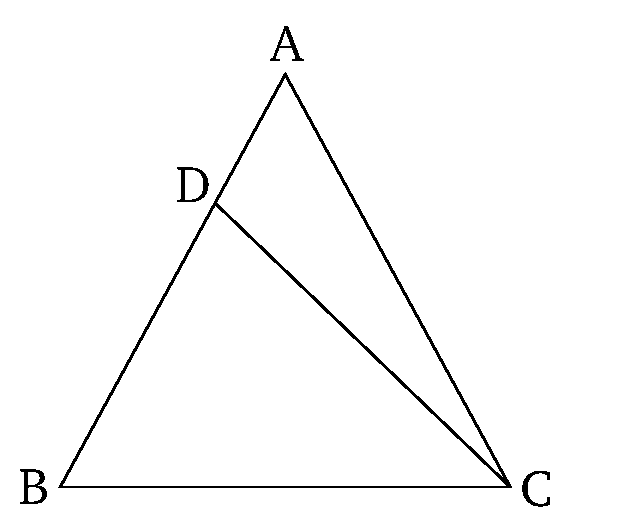
\includegraphics[width=0.5\linewidth]{figures/fig06e.eps}
    \label{fig:prop_6}
    \end{center}
\end{figure*}

If a triangle has two angles equal to one another then the sides subtending the
equal angles will also be equal to one another.

Let $ABC$ be a triangle having the angle $ABC$ equal to the angle $ACB$. I say that
side $AB$ is also equal to side $AC$.

For if $AB$ is unequal to $AC$ then one of them is greater. Let $AB$ be greater. And
let $DB$, equal to the lesser $AC$, have been cut off from the greater $AB$ [Prop.~1.3].  And
let $DC$ have been joined [Post.~\ref{post:1}].

Therefore, since $DB$ is equal to $AC$, and $BC$ (is) common, the two sides $DB$, $BC$ are equal to the two sides $AC$, $CB$, respectively, and the angle $DBC$
is equal to the angle $ACB$. Thus, the base $DC$ is equal to the base
$AB$, and the triangle $DBC$ will be equal to the triangle $ACB$ [Prop.~1.4], the lesser
to the greater. The very notion (is) absurd [C.N.~\ref{cn:5}]. Thus, $AB$ is not unequal
to $AC$. Thus, (it is) equal.

Thus, if a triangle has two angles equal to one another then the sides subtending the
equal angles will also be equal to one another. (Which is) the very thing it was required to show.


\section*{Commentary}

\begin{proposition}\label{proposition_6}\lean{Elements.Book1.proposition_6}\leanok
    In $\triangle ABC$, if $\angle~ABC = \angle~ACB$, then $|AB| = |AC|$.
\end{proposition}
\begin{proof}
    \uses{proposition_3,proposition_4}\leanok
    See the original proof by Euclid.
\end{proof}

\chapter*{Proposition 7}
\label{prop:7}

\begin{figure*}[ht]
    \begin{center}
    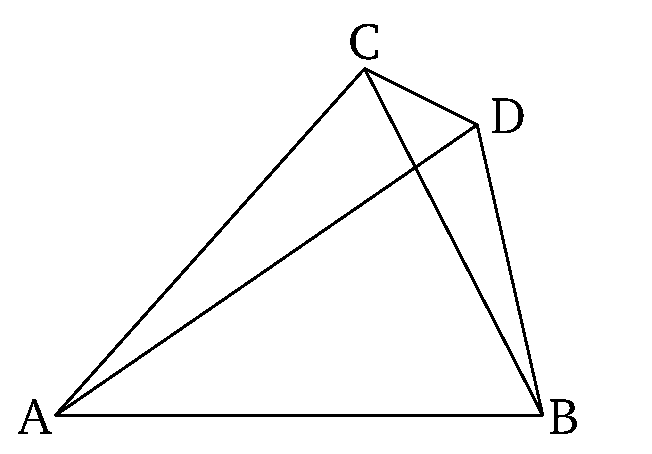
\includegraphics[width=0.5\linewidth]{figures/fig07e.eps}
    \label{fig:prop_7}
    \end{center}
\end{figure*}

On the same straight-line, two other straight-lines 
equal, respectively, to 
two (given) straight-lines (which meet) cannot be constructed (meeting)
at  a different point on the same
side (of the straight-line), but having the same ends as the given straight-lines.

For, if possible, let the two straight-lines $AC$, $CB$, equal to two other straight-lines $AD$, $DB$, respectively, have been constructed
on the same straight-line $AB$, meeting at different points, $C$ and $D$, on the
same side (of $AB$), and having the same ends (on $AB$). So $CA$ is equal to $DA$, having the same end $A$ as it, and $CB$ is equal to $DB$, having the
same end $B$ as it. And let $CD$ have been joined [Post.~\ref{post:1}].

Therefore, since $AC$ is equal to $AD$,  the angle $ACD$ is also equal to angle $ADC$ [Prop.~1.5].
Thus, $ADC$ (is) greater than $DCB$ [C.N.~\ref{cn:5}]. Thus, $CDB$ is much greater
than $DCB$ [C.N.~\ref{cn:5}]. Again, since  $CB$ is equal to $DB$, the angle $CDB$ is also equal to
angle $DCB$ [Prop.~1.5]. But it was shown that the former (angle) is also much
greater (than the latter). The very thing is impossible.

Thus, on the same straight-line, two other straight-lines equal, respectively, to  
two (given) straight-lines  (which meet) cannot be constructed (meeting)
at a different point on the same
side (of the straight-line), but having the same ends as the given straight-lines.
(Which is) the very thing it was required to show.


\section*{Commentary}

\begin{proposition}\label{proposition_7}\lean{Elements.Book1.proposition_7}\leanok
    $A$ and $B$ are two distinct points on a line $AB$. It is impossible to construct two distinct points $C$ and $D$ on the same side of $AB$, s.t., $|AC| = |AD|$ and $|CB| = |DB|$.
\end{proposition}
\begin{proof}
    \uses{proposition_5}\leanok
    Euclid's proof only works with the last two conditions, though he probably intended to prove a stronger version of Prop.~\ref{proposition_7} without these conditions, i.e., Prop.~\ref{proposition_7} below.
    To get there, we need to enumerate four possible cases (or two modulo permutations), whereas Euclid only considered the first one. 
    \begin{enumerate}
        \item[] $A$, $B$ are on the same of $CD$; $B$, $D$ are on the same side of $AC$: See Euclid's original proof.
        \item[] $A$, $B$ are on different sides of $CD$; $B$, $D$ are on the same side of $AC$: As Fig.~\ref{fig:prop_7'} shows, extend $AC$ to $E$ and $AD$ to $F$. Apply Prop.~\ref{proposition_5} to $\triangle ACD$ to derive $\angle~DCE = \angle~CDF$. Apply Prop.~\ref{proposition_5'} to $\triangle~BCD$ to derive $\angle~BCD = \angle~BDC$. Note that $\angle~DCE~>~\angle~BCD = \angle~BDC~>~\angle~CDF$. Contradiction. 
        \item[] $A$, $B$ are on the same side of $CD$; $B$, $D$ are on different sides of $AC$: Same as Euclid's proof, with $C$ and $D$ swapped.
        \item[] $A$, $B$ are on different sides of $CD$; $B$, $D$ are on different sides of $AC$: Same as Case 2, with $C$ and $D$ swapped.
    \end{enumerate}
\end{proof}


\begin{figure*}[ht]
    \begin{center}
    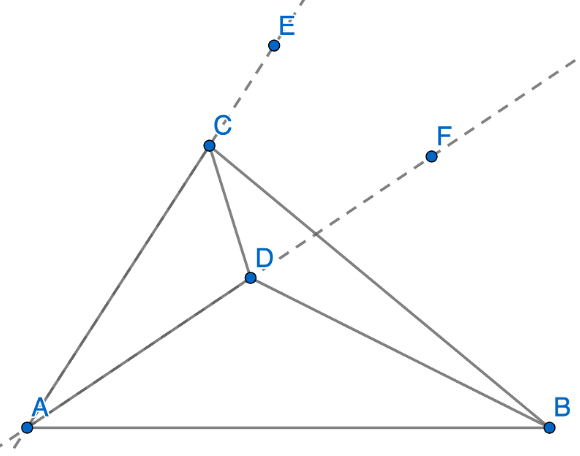
\includegraphics[width=0.5\linewidth]{figures/proposition_7'.png}
    \label{fig:prop_7'}
    \caption{$A$ and $B$ are on different sides of $CD$. $B$ and $D$ are on the same side of $AC$.}
    \end{center}
\end{figure*}

\begin{figure*}[ht]
    \begin{center}
    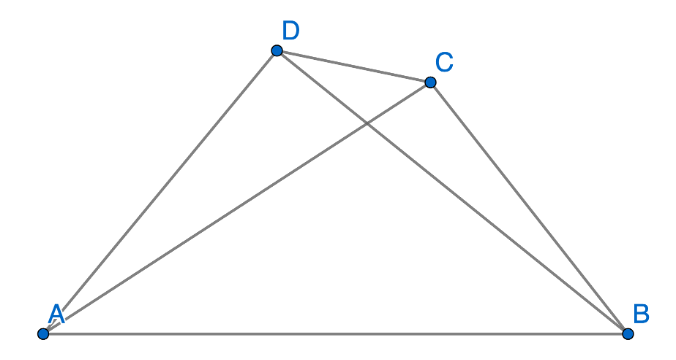
\includegraphics[width=0.5\linewidth]{figures/proposition_7''.png}
    \label{fig:prop_7''}
    \caption{$A$ and $B$ are on the same side of $CD$. $B$ and $D$ are on different sides of $AC$.}
    \end{center}
\end{figure*}

\begin{figure*}[ht]
    \begin{center}
    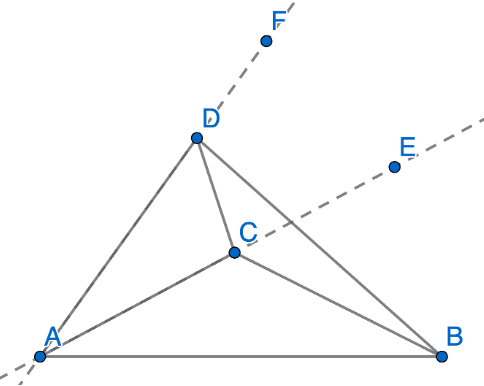
\includegraphics[width=0.5\linewidth]{figures/proposition_7'''.png}
    \label{fig:prop_7'''}
    \caption{$A$ and $B$ are on different sides of $CD$. $B$ and $D$ are on different sides of $AC$.}
    \end{center}
\end{figure*}

\chapter*{Proposition 8}
\label{prop:8}

\begin{figure*}[ht]
    \begin{center}
    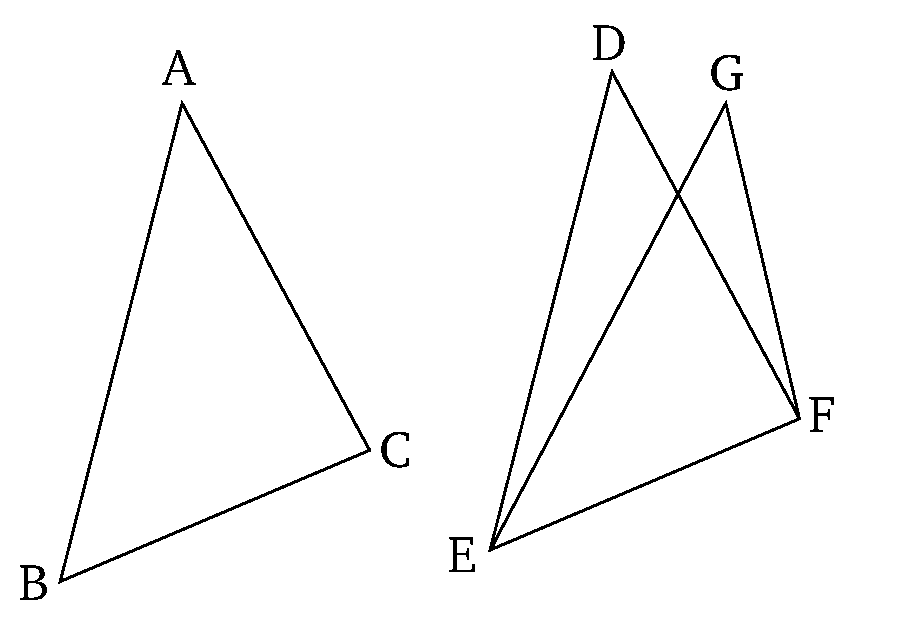
\includegraphics[width=0.5\linewidth]{figures/fig08e.eps}
    \label{fig:prop_8}
    \end{center}
\end{figure*}

If two triangles have  two sides equal to two sides, respectively, 
and also have the base equal to the base, then they will
also have equal the angles  encompassed by
the equal straight-lines.

Let $ABC$ and $DEF$ be two triangles having the two sides $AB$ and $AC$ equal to the two
sides $DE$ and $DF$, respectively. (That is) $AB$ to $DE$, and $AC$ to $DF$.  Let them also have
the base $BC$ equal to the base $EF$. I say that the angle $BAC$ is also equal
to the angle $EDF$.

For if triangle $ABC$ is applied to triangle $DEF$, the point $B$ being placed on
point $E$, and the straight-line $BC$ on $EF$, then point $C$ will also coincide with $F$, on
account of $BC$ being equal to $EF$.
So  (because of) $BC$ coinciding with $EF$,  (the sides) $BA$ and $CA$ will also
coincide with  $ED$ and $DF$ (respectively). 
For if base $BC$ coincides with base $EF$, but the sides $AB$ and $AC$ 
do not coincide with $ED$ and $DF$ (respectively), but miss like $EG$
and $GF$ (in the above figure), 
then we will have constructed upon the same straight-line, two other straight-lines equal, respectively, to two (given) straight-lines,  and (meeting)
at a different point on the same
side (of the straight-line), but having the same ends. But (such straight-lines) cannot be constructed [Prop.~1.7].
Thus,  the base $BC$ being applied to the  base $EF$,  the sides $BA$ and $AC$
cannot not coincide with $ED$ and $DF$ (respectively). Thus, they
will coincide. So the angle $BAC$ will also coincide with angle $EDF$,
and will be equal to it [C.N.~\ref{cn:4}].

Thus, if two triangles have  two  sides equal to two side, respectively,
and  have the base equal to the base, then they will also have equal the angles  encompassed by
the equal straight-lines. (Which is) the very thing it was required to show.


\section*{Commentary}

\begin{proposition}\label{proposition_8}\lean{Elements.Book1.proposition_8}\leanok
    $\triangle~ABC$ and $\triangle~DEF$ are two triangles with $AB = DE$, $AC = DF$, and $BC = EF$. Then, $\angle~BAC = \angle~EDF$.
\end{proposition}
\begin{proof}
    \uses{proposition_7}\leanok
    See the original proof by Euclid.
\end{proof}

\chapter*{Proposition 9}
\label{prop:9}


\begin{figure*}[ht]
    \begin{center}
    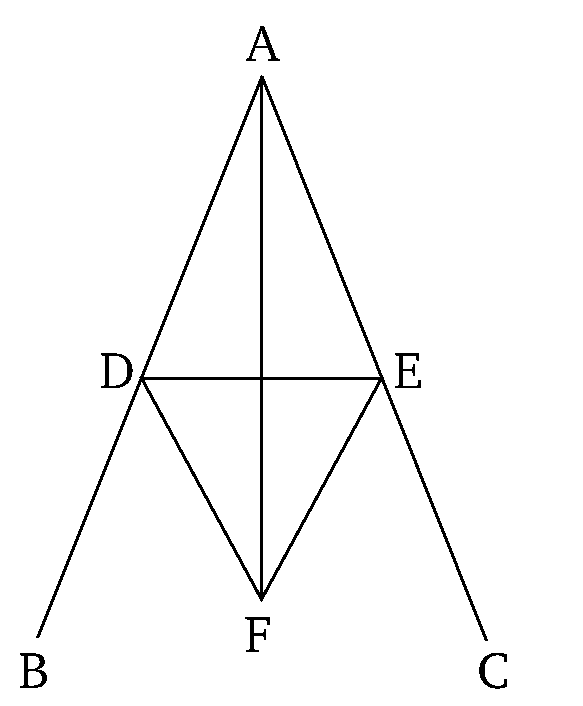
\includegraphics[width=0.5\linewidth]{figures/fig09e.eps}
    \label{fig:prop_9}
    \end{center}
\end{figure*}

To cut a given rectilinear angle in half.

Let $BAC$ be the given rectilinear angle. So it is required to
cut it in half.

Let the point $D$ have been taken at random on $AB$,
and let $AE$, equal to $AD$,  have been cut off from $AC$  [Prop.~1.3], and
let $DE$ have been joined. And let the equilateral triangle $DEF$
have been constructed upon $DE$ [Prop.~1.1], and let $AF$ have been
joined. I say that the angle $BAC$ has been cut in half by the straight-line
$AF$.

For since $AD$ is equal to  $AE$, and $AF$ is common, the two (straight-lines) $DA$,
$AF$ are equal to the two (straight-lines) $EA$, $AF$, respectively. And the base $DF$
is equal to the base $EF$. Thus, angle $DAF$ is equal to angle $EAF$ [Prop.~1.8].

Thus, the given rectilinear angle $BAC$ has been cut in half by the
straight-line $AF$. (Which is) the very thing it was required to do.


\section*{Commentary}

\begin{proposition}\label{proposition_9}\lean{Elements.Book1.proposition_9}\leanok
    Given an $\angle~BAC$, there must exist a point $F$, s.t., $F \neq A$ and $\angle~BAF = \angle~CAF$.
\end{proposition}
\begin{proof}
    \uses{proposition_1',proposition_3,proposition_5,proposition_5',proposition_7,proposition_8}\leanok
    Euclid's proof has two problems. First, when constructing $F$, it fails to state the requirement that $F$ and $A$ must be on different sides of $DE$.
    Second, Euclid did not rule out the possibility that $F$ lies on $AB$ or $AC$. If that could happen, 
    $\triangle~DAF$ or $\triangle~EAF$ wouldn't have existed, and the original proof would have failed.

    To prove $F$ is not on $AB$, let's first assume $F$ is on $AB$ (Fig.~\ref{fig:prop_9}). Apply Prop.~\ref{proposition_5} to $\triangle~ADE$ to derive $\angle~FDE = \angle~CED$. Apply Prop.~\ref{proposition_5'} to $\triangle~FDE$ to derive $\angle~FDE = \angle~FED$. Note that $\angle~CED~>~\angle~FED$. Contradiction.

    Similarly, we can prove $F$ is not on $AC$.
\end{proof}

\begin{figure*}[ht]
    \begin{center}
    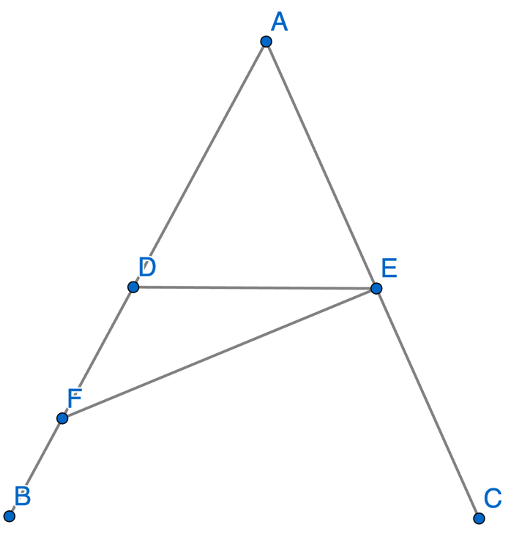
\includegraphics[width=0.5\linewidth]{figures/proposition_9.png}
    \label{fig:prop_9}
    \caption{$F$ on $AB$ cannot be true.}
    \end{center}
\end{figure*}

We can derive two additional properties of $F$: First, $F$ and $C$ must be on the same side of $AB$. Second, $F$ and $B$ must be on the same side of $AC$. 
Euclid did not include them in Prop.~\ref{proposition_9}, but they are necessary for later proofs.

\begin{proposition}\label{proposition_9'}\lean{Elements.Book1.proposition_9'}\leanok
    Given an $\angle~BAC$, there must exist a point $F$, s.t., $F \neq A$, $\angle~BAF = \angle~CAF$; $F$, $C$ are on the same side of $AB$; and $F$, $B$ are on the same side of $AC$.
\end{proposition}
\begin{proof}
    \uses{proposition_1',proposition_3,proposition_5,proposition_5',proposition_7,proposition_8}\leanok
    Same as the proof of Prop.~\ref{proposition_9}.
\end{proof}
\chapter*{Proposition 10}
\label{prop:10}

\begin{figure*}[ht]
    \begin{center}
    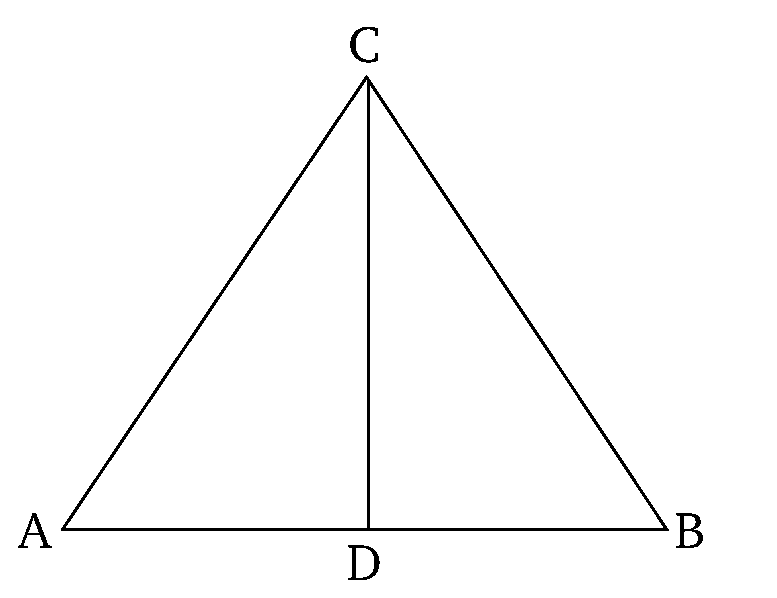
\includegraphics[width=0.5\linewidth]{figures/fig10e.eps}
    \label{fig:prop_10}
    \end{center}
\end{figure*}

To cut a given finite straight-line in half.

Let $AB$ be the given finite straight-line. So it is required to cut the
finite straight-line $AB$ in half.

Let the equilateral triangle $ABC$ have been constructed upon  ($AB$)
[Prop.~1.1], and let the angle $ACB$ have been cut in half by the
straight-line $CD$ [Prop.~1.9]. I say that the straight-line $AB$ has been
cut in half at  point $D$.

For since $AC$ is equal to $CB$, and $CD$ (is) common, the two (straight-lines) $AC$, $CD$
are equal to the two (straight-lines) $BC$, $CD$, respectively. And the angle $ACD$ is
equal to the angle $BCD$. Thus, the base $AD$ is equal to the base $BD$
[Prop.~1.4].

Thus, the given finite straight-line $AB$ has been cut in half at  (point) $D$. 
(Which is) the
very thing it was required to do.


\section*{Commentary}

\begin{proposition}\label{proposition_10}\lean{Elements.Book1.proposition_10}\leanok
    $A$ and $B$ are two distinct points on a line $AB$. There must exist a point $D$ between them, s.t., $|AD| = |DB|$.
\end{proposition}
\begin{proof}
    \uses{proposition_1,proposition_4,proposition_9'}\leanok
    See the original proof by Euclid.
\end{proof}

\chapter*{Proposition 11}
\label{prop:11}


\begin{figure*}[ht]
    \begin{center}
    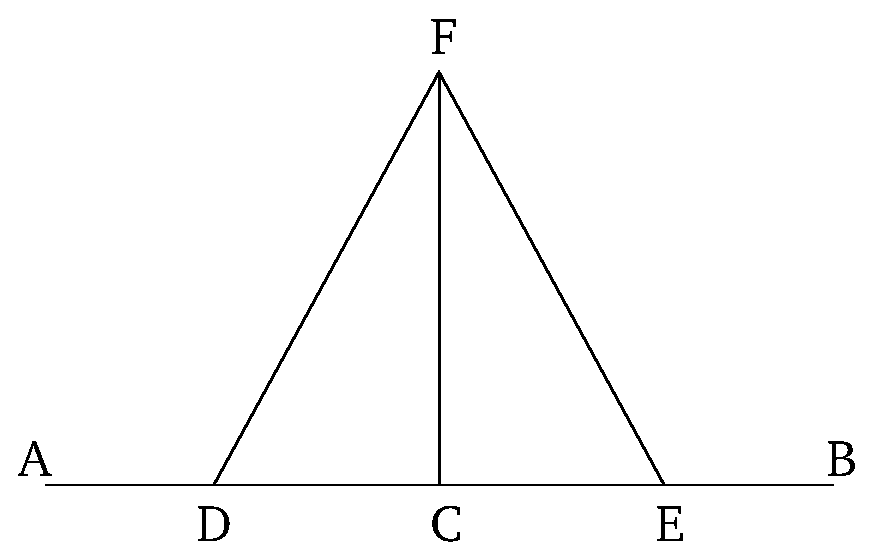
\includegraphics[width=0.5\linewidth]{figures/fig11e.eps}
    \label{fig:prop_11}
    \end{center}
\end{figure*}

To draw a straight-line at right-angles to a given straight-line from a given point on it.

Let $AB$ be the given straight-line, and $C$ the given point on it. So it is required
to draw a straight-line from the point $C$ at right-angles to the straight-line $AB$.

Let the point $D$ be have been taken at random on $AC$, and let $CE$ be made equal to $CD$ [Prop.~1.3], and let the equilateral triangle $FDE$
have been constructed on $DE$ [Prop.~1.1], and let $FC$ have been
joined. I say that the straight-line $FC$ has been drawn at right-angles
to the given straight-line $AB$ from the given point $C$ on it.

For since $DC$ is equal to $CE$, and $CF$ is common, the two (straight-lines) $DC$, $CF$
are equal to the two (straight-lines), $EC$, $CF$, respectively.  And the base $DF$
is equal to the base $FE$. Thus, the angle $DCF$ is equal to the
angle $ECF$ [Prop.~1.8], and they are adjacent. But when a straight-line stood on 
a(nother) straight-line makes the adjacent angles equal to one another, each of the
equal angles is a right-angle [Def.~\ref{def:10}]. Thus, each of the (angles)
$DCF$ and $FCE$ is a right-angle.

Thus, the straight-line $CF$ has been drawn at right-angles to the
given straight-line $AB$ from the given point $C$ on it. (Which is) the very thing
it was required to do.


\section*{Commentary}

\begin{proposition}\label{proposition_11}\lean{Elements.Book1.proposition_11}\leanok
    $A$, $B$ are two distinct points on a line $AB$. $C$ is a point between them. Then, there must exist a point $F$ not on $AB$, s.t., $\angle~ACF$ is a right angle.
\end{proposition}
\begin{proof}
    \uses{proposition_1,proposition_3,proposition_8}\leanok
    See the original proof by Euclid.
\end{proof}

Euclid did not explicitly state that $F$ can be constructed on any side of $AB$, which is useful for later proofs.

\begin{proposition}\label{proposition_11'}\lean{Elements.Book1.proposition_11'}\leanok
    $A$, $B$ are two distinct points on a line $AB$. $C$ is a point between them, and $X$ is a point not on $AB$. Then, there must exist a point $F$ on the same side of $AB$ with $X$, s.t., $\angle~ACF$ is a right angle.
\end{proposition}
\begin{proof}
    \uses{proposition_1',proposition_3,proposition_8}\leanok
    Similar to the original proof by Euclid.
\end{proof}

Euclid's proof seems to assume $A$ and $B$ to be infinite points (so any point $C$ on the line $AB$ is between $A$ and $B$). However, infinite points are not supported in E. We need the following proposition to get around this issue.

\begin{proposition}\label{proposition_11''}\lean{Elements.Book1.proposition_11''}\leanok
    For two distinct points $A$ and $B$ on a line $AB$, there must exist a point $F$ not on $AB$, s.t., $\angle~FAB$ is a right angle.
\end{proposition}
\begin{proof}
    \uses{proposition_11}\leanok
    Let $C$ be a point on $AB$, s.t., $A$ is between $B$ and $C$. Apply Prop.~\ref{proposition_11}.
\end{proof}

Similarly, $F$ can be constructed on either side.


\begin{proposition}\label{proposition_11'''}\lean{Elements.Book1.proposition_11'''}\leanok
    $A$, $B$ are two distinct points on a line $AB$. $X$ is a point not on $AB$. Then, there must exist a point $F$ on a different side of $AB$ from $X$, s.t., $\angle~FAB$ is a right angle.
\end{proposition}
\begin{proof}
    \uses{proposition_11'}\leanok
    Let $C$ be a point on $AB$, s.t., $A$ is between $B$ and $C$. Let $Y$ be any point on the different side of $AB$ from $X$. Apply Prop.~\ref{proposition_11'}.
\end{proof}

\chapter*{Proposition 12}
\label{prop:12}

\begin{figure*}[ht]
    \begin{center}
    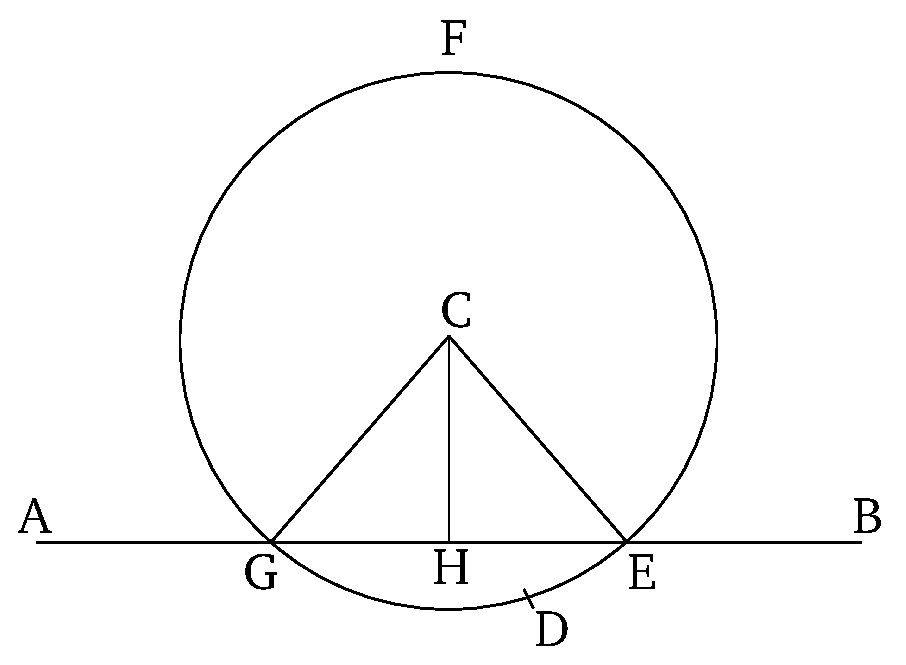
\includegraphics[width=0.5\linewidth]{figures/fig12e.eps}
    \label{fig:prop_12}
    \end{center}
\end{figure*}

To draw a straight-line perpendicular to a given infinite straight-line from a given point which is not
on it.\\

Let $AB$ be the given infinite straight-line  and $C$ the given point, which is not
on ($AB$). So it is required to draw a  straight-line  perpendicular to the
given infinite straight-line $AB$ from the given point $C$, which is not on
($AB$).

For let point $D$ have been taken at random on the other side (to $C$) of 
the straight-line $AB$, and let the circle $EFG$ have been drawn
with center $C$ and radius $CD$ [Post.~\ref{post:3}], and let the straight-line $EG$ have been cut
in half at (point) $H$ [Prop.~1.10], and let the straight-lines $CG$, $CH$,
and $CE$ have been joined. I say that the  (straight-line) $CH$ has
been drawn  perpendicular to the given infinite straight-line
$AB$ from the given point $C$, which is not on ($AB$).

For since $GH$ is equal to $HE$, and $HC$ (is) common, the two (straight-lines) $GH$, 
$HC$
are equal to the two (straight-lines) $EH$, $HC$, respectively, and the base $CG$ is
equal to the base $CE$. Thus, the angle $CHG$ is equal to the
angle $EHC$ [Prop.~1.8], and they are adjacent. But when a straight-line
stood on a(nother) straight-line makes the adjacent angles equal to one another, each of the equal angles is a right-angle, and the former straight-line is called a perpendicular to that upon which it stands [Def.~\ref{def:10}].

Thus, the (straight-line) $CH$ has been drawn perpendicular to the given infinite straight-line $AB$ from the given point $C$, which is not
on  ($AB$). (Which is) the very thing it was required to do.


\section*{Commentary}

\begin{proposition}\label{proposition_12}\lean{Elements.Book1.proposition_12}\leanok
    $A$ and $B$ are two distinct points on a line $AB$. $C$ is a point not on $AB$. Then, there must exist a point $H$ on $AB$ s.t., $\angle~AHC$ or $\angle~BHC$ is a right angle.
\end{proposition}
\begin{proof}
    \uses{proposition_8,proposition_10}\leanok
    See the original proof by Euclid.
\end{proof}

\chapter*{Proposition 13}
\label{prop:13}

\begin{figure*}[ht]
    \begin{center}
    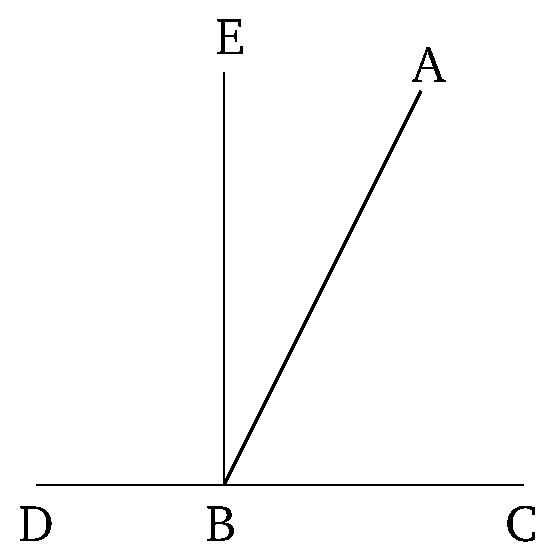
\includegraphics[width=0.5\linewidth]{figures/fig13e.eps}
    \label{fig:prop_13}
    \end{center}
\end{figure*}

If a straight-line stood on a(nother)  straight-line makes angles,
it will certainly either make two right-angles, or (angles whose sum is) equal
to two right-angles. 

For  let some straight-line $AB$ stood on the straight-line $CD$ make the
angles $CBA$ and $ABD$. I say that the angles $CBA$ and $ABD$ are
certainly either two right-angles, or (have a sum) equal to two right-angles.

In fact, if $CBA$ is equal to $ABD$ then they are two right-angles [Def.~\ref{def:10}].
But, if not, let $BE$ have been drawn from the point $B$ at right-angles to [the
straight-line] $CD$ [Prop.~1.11]. Thus, $CBE$ and $EBD$ are two right-angles.
And since $CBE$ is equal to the two (angles) $CBA$ and $ABE$, let $EBD$ have been added
to both. Thus, the (sum of the angles) $CBE$ and $EBD$ is equal to the  (sum of the) three (angles)
$CBA$, $ABE$, and $EBD$ [C.N.~\ref{cn:2}]. Again, since $DBA$ is equal to the two (angles) $DBE$
and $EBA$, let $ABC$ have been added to both. Thus, the (sum of the angles) $DBA$ and $ABC$ is
equal to the (sum of the) three (angles) $DBE$, $EBA$, and $ABC$ [C.N.~\ref{cn:2}]. But (the sum of) $CBE$ and $EBD$ was
also shown (to be) equal to the (sum of the) same three (angles). And things equal to the
same thing are also equal to one another [C.N.~\ref{cn:1}]. Therefore, 
(the sum of) $CBE$ and
$EBD$ is also equal to (the sum of) $DBA$ and $ABC$. But, (the sum of) $CBE$ and $EBD$ is two
right-angles. Thus, (the sum of) $ABD$ and $ABC$ is also equal to two right-angles.

Thus, if a straight-line stood on a(nother)  straight-line makes angles,
it will certainly either make two right-angles, or (angles whose sum is) equal
to two right-angles. (Which is) the very thing it was required to show.



\section*{Commentary}

\begin{proposition}\label{proposition_13}\lean{Elements.Book1.proposition_13}\leanok
    $A$, $B$ are two distinct points on a line $AB$. $C$, $D$ are two distinct points on a different line $CD$. $B$ is between $C$ and $D$. Then, we have $\angle~CBA + \angle~ABD$ is 180 degrees.
\end{proposition}
\begin{proof}
    \uses{proposition_11'}\leanok
    See the original proof by Euclid.
\end{proof}

\chapter*{Proposition 14}
\label{prop:14}

\begin{figure*}[ht]
    \begin{center}
    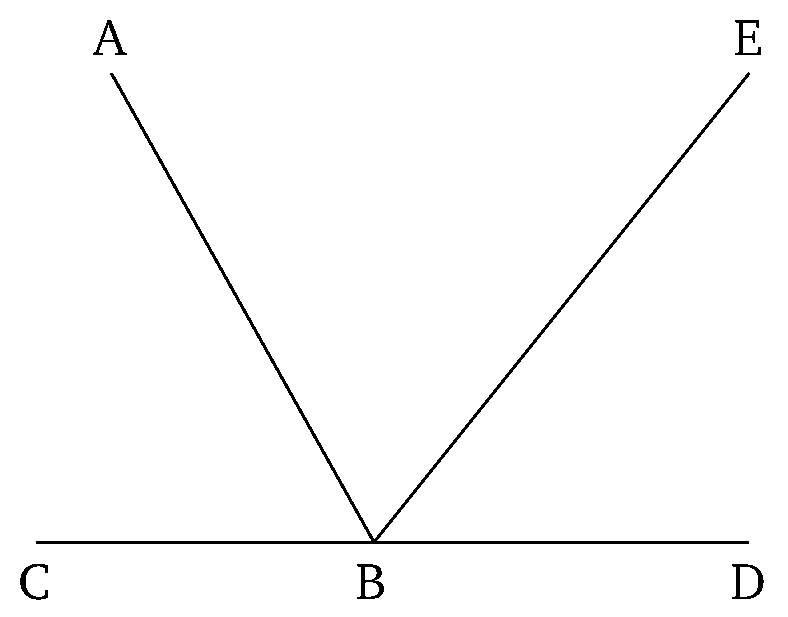
\includegraphics[width=0.5\linewidth]{figures/fig14e.eps}
    \label{fig:prop_14}
    \end{center}
\end{figure*}

If two straight-lines, not lying on the same side,  make adjacent angles (whose sum is) equal to two right-angles  with some straight-line, at a point on it, then the two straight-lines
will be straight-on (with respect) to one another.

For let two
straight-lines $BC$ and $BD$, not lying on the same side,  make adjacent angles $ABC$ and $ABD$ (whose sum is)
equal to two right-angles with some straight-line $AB$, at the point $B$ on it. I say
that $BD$ is  straight-on with respect to $CB$.

For if $BD$ is not straight-on to $BC$ then let $BE$ be straight-on to $CB$.

Therefore, since the straight-line $AB$ stands on the straight-line $CBE$, the (sum of the) angles $ABC$ and $ABE$ is thus equal to two right-angles [Prop.~1.13]. But (the sum of) $ABC$ and $ABD$ is also equal to two right-angles.
Thus, 
(the sum of angles) $CBA$ and $ABE$ is equal to (the sum of angles) $CBA$ and $ABD$ [C.N.~\ref{cn:1}]. Let (angle)
$CBA$ have been subtracted from both. Thus, the remainder $ABE$ is
equal to the remainder $ABD$ [C.N.~\ref{cn:3}], the lesser to the greater. The very thing is impossible. Thus, $BE$ is not straight-on with respect to $CB$. Similarly, we can
show that neither (is) any other (straight-line)   than $BD$.
Thus, $CB$ is straight-on with respect to $BD$.

Thus, if two straight-lines, not lying on the same side,  make adjacent angles (whose sum is) equal to two right-angles with some straight-line, at a point on it, then the two straight-lines
will be straight-on (with respect) to one another. (Which is) the very thing it
was required to show.


\section*{Commentary}

\begin{proposition}\label{proposition_14}\lean{Elements.Book1.proposition_14}\leanok
    $A$, $B$ are two distinct points on a line $AB$. $C$ and $D$ are two points on different sides of $AB$. $B$, $C$ are on a line $BC$. $B$, $D$ are on a line $BD$. $\angle~ABC + \angle~ABD$ is 180 degrees. Then, $BC$ and $BD$ must be the same line.
\end{proposition}
\begin{proof}
    \uses{proposition_13}\leanok
    Euclid only discussed the case where $E$ and $A$ are on the same side of $BD$, though the proof for other case is almost identical. 
\end{proof}

\chapter*{Proposition 15}
\label{prop:15}

\begin{figure*}[ht]
    \begin{center}
    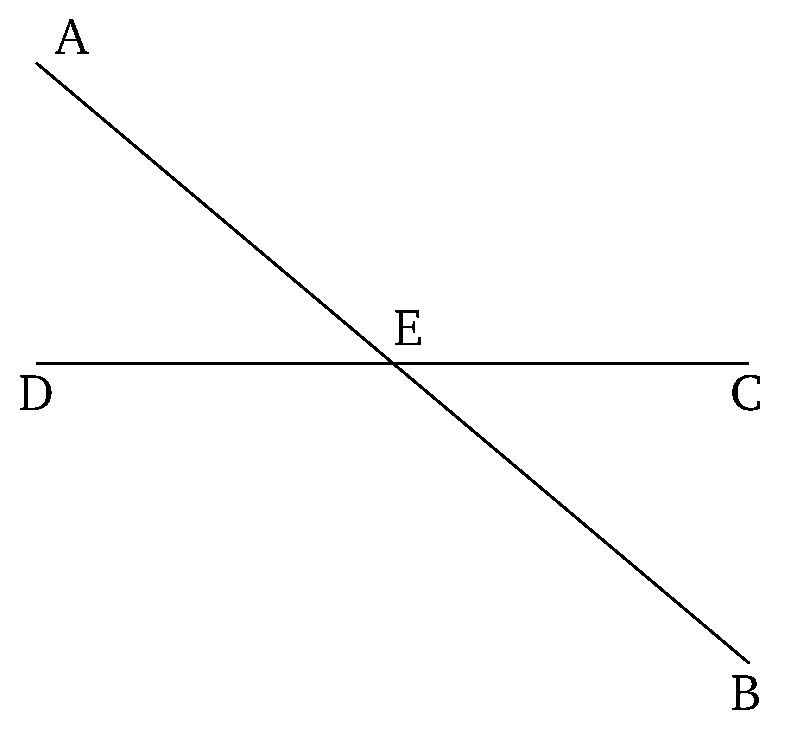
\includegraphics[width=0.5\linewidth]{figures/fig15e.eps}
    \label{fig:prop_15}
    \end{center}
\end{figure*}

If two straight-lines cut one another then they make the vertically opposite angles
equal to one another.

For let the two straight-lines $AB$ and $CD$ cut one another at the point $E$. I say
that  angle $AEC$ is equal to (angle) $DEB$, and (angle) $CEB$ to (angle) $AED$.

For since the straight-line $AE$ stands on the straight-line $CD$, making the
angles $CEA$ and $AED$, the (sum of the) angles $CEA$ and $AED$ is thus equal to two
right-angles [Prop.~1.13]. Again, since the straight-line $DE$ stands on the
straight-line $AB$, making the angles $AED$ and $DEB$, the (sum of the) angles $AED$ and
$DEB$ is thus equal to two right-angles [Prop.~1.13]. But (the sum of) $CEA$ and $AED$ was also shown
(to be) equal to two right-angles. Thus, (the sum of) $CEA$ and $AED$ is equal to (the sum of) $AED$ and $DEB$ [C.N.~\ref{cn:1}]. Let $AED$ have been subtracted from both. Thus, the remainder
$CEA$ is equal to the remainder $BED$ [C.N.~\ref{cn:3}]. Similarly, it can be shown that
$CEB$ and $DEA$ are also equal.

Thus, if two straight-lines cut one another then they make the vertically opposite angles
equal to one another. (Which is) the very thing it was required to show.


\section*{Commentary}

\begin{proposition}\label{proposition_15}\lean{Elements.Book1.proposition_15}\leanok
    $AB$ and $CD$ are two different lines intersecting at $E$. $A$ and $B$ are two distinct points on $AB$. $C$ and $D$ are two distinct points on $CD$. $E$ is between $A$ and $B$, and $E$ is also between $C$ and $D$. Then, we have $\angle~AEC = \angle~DEB$ and $\angle~CEB = \angle~AED$.
\end{proposition}
\begin{proof}
    \uses{proposition_13}\leanok
    See the original proof by Euclid.
\end{proof}

\chapter*{Proposition 16}
\label{prop:16}

\begin{figure*}[ht]
    \begin{center}
    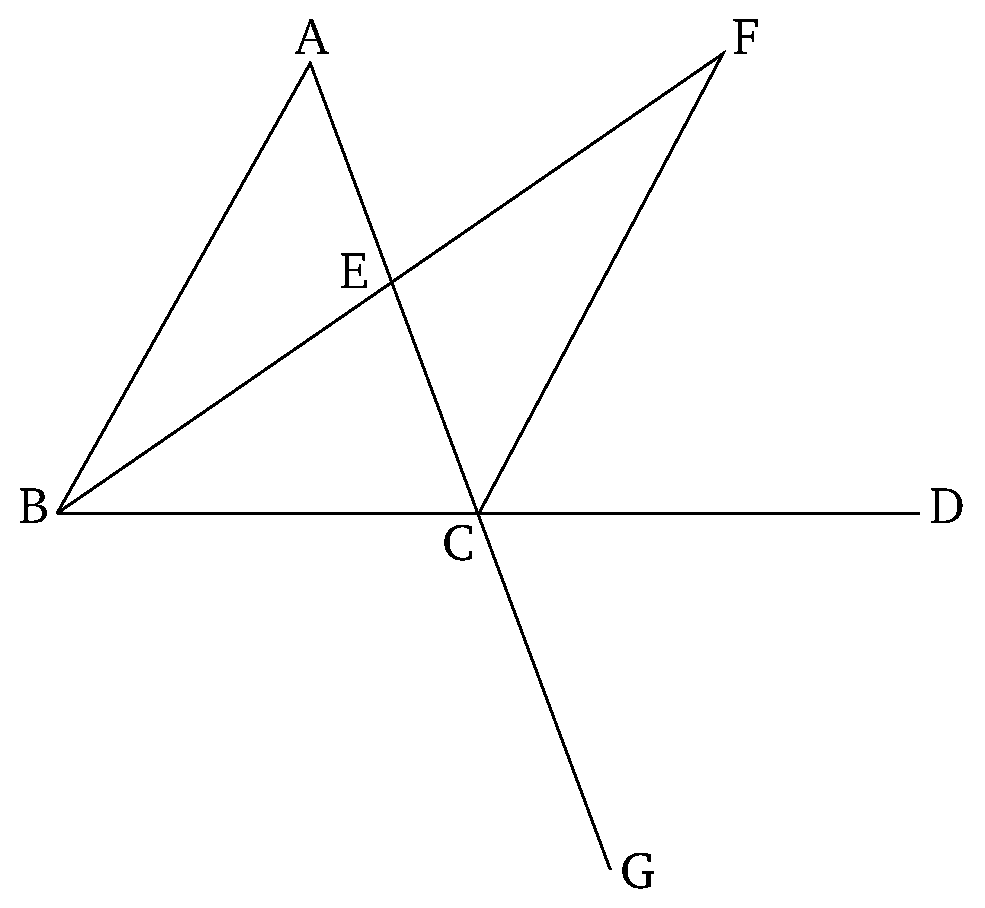
\includegraphics[width=0.5\linewidth]{figures/fig16e.eps}
    \label{fig:prop_16}
    \end{center}
\end{figure*}

For any triangle, when one of the sides is produced, the external angle
is greater than each of the internal and opposite angles.

Let $ABC$ be a triangle, and let one of its sides $BC$ have been produced 
 to $D$. I say that the external angle $ACD$ is greater than each of the
 internal and opposite angles, $CBA$ and $BAC$.
 
Let the (straight-line) $AC$ have been cut in half at (point) $E$ [Prop.~1.10].
 And $BE$ being joined, let it have been produced in a straight-line to
 (point) $F$. And let $EF$ be made equal to $BE$ [Prop.~1.3], and let $FC$ have been joined, and let $AC$ have been drawn through to (point) $G$.

Therefore, since $AE$ is equal to $EC$, and $BE$ to $EF$, the two (straight-lines)
 $AE$, $EB$ are equal to the two (straight-lines) $CE$, $EF$, respectively. 
 Also, angle $AEB$ is equal to angle $FEC$, for (they are)
 vertically opposite [Prop.~1.15]. Thus, the base $AB$ is equal to the base
 $FC$, and the triangle $ABE$ is equal to the triangle $FEC$, and the remaining
 angles subtended by the equal sides are equal to the corresponding remaining angles [Prop.~1.4]. Thus, $BAE$ is equal to $ECF$. But $ECD$ is greater than $ECF$. Thus,
 $ACD$ is greater than $BAE$. Similarly, by having cut $BC$ in half,  it can  be shown (that) $BCG$---that is to say, $ACD$---(is) also greater than $ABC$.
 
Thus, for any triangle, when one of the sides is produced, the external angle
is greater than each of the internal and opposite angles. (Which is) the very thing
it was required to show.


\section*{Commentary}

\begin{proposition}\label{proposition_16}\lean{Elements.Book1.proposition_16}\leanok
    $BC$ is an edge of $\triangle~ABC$ and is extended to $D$. Then, we have $\angle~ACD~>~\angle~CBA$ and $\angle~ACD~>~\angle~BAC$.
\end{proposition}
\begin{proof}
    \uses{proposition_3,proposition_4,proposition_10,proposition_15}\leanok
    Euclid only proved $\angle~ACD~>~\angle~CBA$, though the proof of $\angle~ACD~>~\angle~BAC$ is almost identical.
\end{proof}

\chapter*{Proposition 17}
\label{prop:17}


\begin{figure*}[ht]
    \begin{center}
    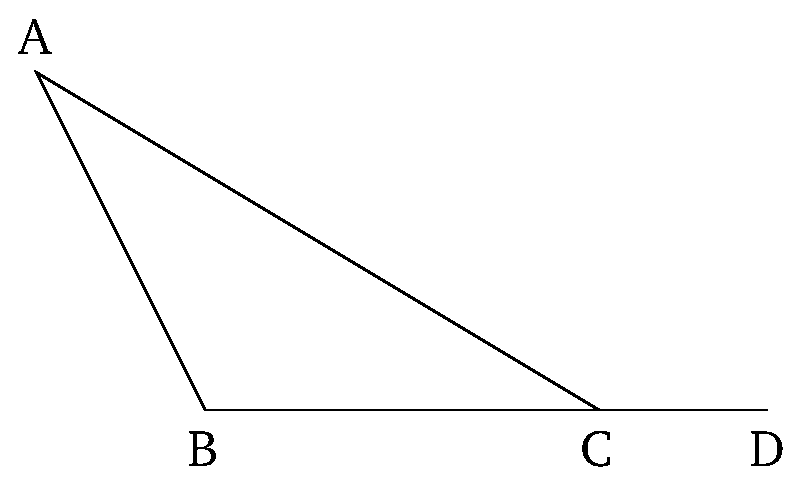
\includegraphics[width=0.5\linewidth]{figures/fig17e.eps}
    \label{fig:prop_17}
    \end{center}
\end{figure*}

For any triangle,  (the sum of) two angles taken together in any (possible way) is less than two right-angles.

Let $ABC$ be a triangle. I say that (the sum of) two angles of triangle $ABC$
taken together in any (possible way) is less than two right-angles.

For let $BC$ have been produced to $D$.

And since the angle $ACD$ is external to triangle $ABC$, it is greater than the
internal and opposite angle $ABC$ [Prop.~1.16]. Let $ACB$ have been added to both. Thus, the
(sum of the angles) $ACD$ and $ACB$ is greater than the  (sum of the angles) $ABC$ and
$BCA$. But, (the sum of) $ACD$ and $ACB$ is equal to two right-angles [Prop.~1.13].
Thus, (the sum of) $ABC$ and $BCA$ is less than two right-angles. Similarly,
we can show that (the sum of) $BAC$ and $ACB$ is also less than two right-angles,
and further (that the sum of) $CAB$ and $ABC$ (is less than two right-angles).

Thus, for any triangle,  (the sum of) two angles taken together in any (possible way) is less than two right-angles. (Which is) the very thing
it was required to show.


\section*{Commentary}

\begin{proposition}\label{proposition_17}\lean{Elements.Book1.proposition_17}\leanok
    In $\triangle~ABC$, we have $\angle~ABC + \angle~BCA$ is less than 180 degrees. 
\end{proposition}
\begin{proof}
    \uses{proposition_13,proposition_16}\leanok
    See the original proof by Euclid.
\end{proof}

\chapter*{Proposition 18}
\label{prop:18}

\begin{figure*}[ht]
    \begin{center}
    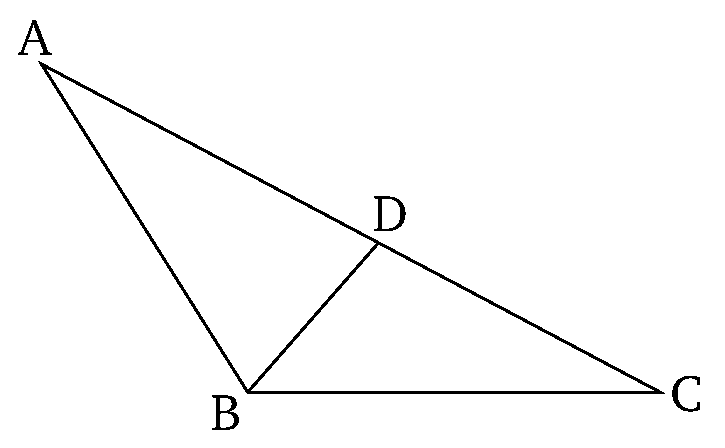
\includegraphics[width=0.5\linewidth]{figures/fig18e.eps}
    \label{fig:prop_18}
    \end{center}
\end{figure*}

In any triangle, the greater side subtends the greater angle.

For let $ABC$ be a triangle having side $AC$ greater than $AB$. I say that
angle $ABC$ is also greater than $BCA$.

For since $AC$ is greater than $AB$, let $AD$ be made equal to $AB$
 [Prop.~1.3],
and let $BD$ have been joined.

And since angle $ADB$ is external to triangle $BCD$, it is greater than the
internal and opposite (angle) $DCB$ [Prop.~1.16]. But $ADB$ (is) equal to $ABD$,
since side $AB$ is also equal to side $AD$ [Prop.~1.5]. Thus,
$ABD$ is also greater than $ACB$. Thus, $ABC$ is much greater than 
$ACB$.

Thus, in any triangle, the greater side subtends the greater angle.
(Which is) the very thing  it was required to show.


\section*{Commentary}

\begin{proposition}\label{proposition_18}\lean{Elements.Book1.proposition_18}\leanok
    In $\triangle~ABC$, if $|AC|~>~|AB|$, then $\angle~ABC~>~\angle~BCA$
\end{proposition}
\begin{proof}
    \uses{proposition_3,proposition_5',proposition_16}\leanok
    See the original proof by Euclid.
\end{proof}

\chapter*{Proposition 19}
\label{prop:19}

\begin{figure*}[ht]
    \begin{center}
    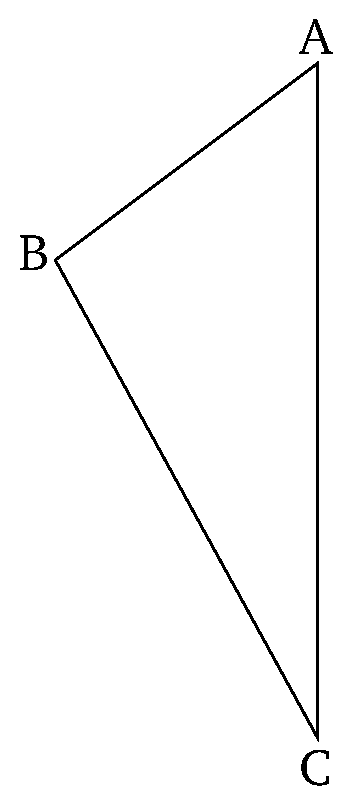
\includegraphics[width=0.5\linewidth]{figures/fig19e.eps}
    \label{fig:prop_19}
    \end{center}
\end{figure*}

In any triangle, the greater angle is subtended by the greater side.

Let $ABC$ be a triangle having the angle $ABC$ greater than $BCA$. I say
that side $AC$ is also greater than side $AB$.

For if not, $AC$ is certainly either equal to, or less than, $AB$. In fact, $AC$ is not
equal to $AB$. For then angle $ABC$  would also have been equal to $ACB$ [Prop.~1.5].
But it is not. Thus, $AC$ is not equal to $AB$.
Neither, indeed, is $AC$ less than $AB$. For then angle $ABC$ would also have been
less than $ACB$ [Prop.~1.18]. But it is not. Thus, $AC$ is not less than
$AB$. But it was  shown that ($AC$) is    not equal (to $AB$) either. Thus, $AC$ 
is greater than $AB$.

Thus, in any triangle, the greater angle is subtended by the greater side.
(Which is) the very thing it was required to show.


\section*{Commentary}

\begin{proposition}\label{proposition_19}\lean{Elements.Book1.proposition_19}\leanok
    In $\triangle~ABC$, if $\angle~ABC~>~\angle~BCA$, then |AC|~>~|AB|.
\end{proposition}
\begin{proof}
    \uses{proposition_5',proposition_18}\leanok
    See the original proof by Euclid.
\end{proof}

\chapter*{Proposition 20}
\label{prop:20}

\begin{figure*}[ht]
    \begin{center}
    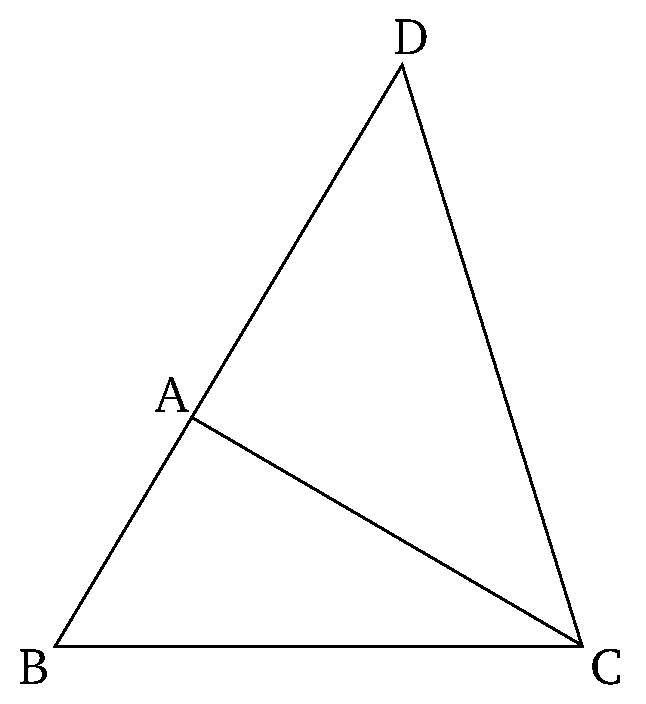
\includegraphics[width=0.5\linewidth]{figures/fig20e.eps}
    \label{fig:prop_20}
    \end{center}
\end{figure*}

In any triangle, (the sum of) two sides taken together in any (possible way) is greater than the remaining (side).

For let $ABC$ be a triangle. I say that in triangle $ABC$ (the sum of) two
sides taken together in
any (possible way) is greater than the remaining (side). (So), (the sum of) $BA$ and $AC$ (is greater) than $BC$,
(the sum of) $AB$ and $BC$ than $AC$, and (the sum of) $BC$ and $CA$ than $AB$.

For let $BA$ have been drawn through to point $D$, and let $AD$ be made equal to $CA$ [Prop.~1.3], and let $DC$ have been joined.

Therefore, since $DA$ is equal to $AC$, the angle $ADC$ is also equal to
$ACD$ [Prop.~1.5]. Thus, $BCD$ is greater than $ADC$. And since
 $DCB$ is a triangle having the angle $BCD$ greater than $BDC$, and the
greater angle subtends the greater side [Prop.~1.19], $DB$ is thus
greater than $BC$. But $DA$ is equal to $AC$. Thus, (the sum of) $BA$ and $AC$ is
greater than $BC$. Similarly, we can show that (the sum of) $AB$ and $BC$ is also
greater than $CA$, and (the sum of) $BC$ and $CA$ than $AB$.

Thus, in any triangle, (the sum of) two sides taken together in any (possible way) is greater than the remaining (side). (Which is) the very thing
it was required to show.


\section*{Commentary}

\begin{proposition}\label{proposition_20}\lean{Elements.Book1.proposition_20}\leanok
    In $\triangle~ABC$, we have $|BA| + |AC|~>~|BC|$.
\end{proposition}
\begin{proof}
    \uses{proposition_3,proposition_5',proposition_19}\leanok
    See the original proof by Euclid.
\end{proof}

\chapter*{Proposition 21}
\label{prop:21}

\begin{figure*}[ht]
    \begin{center}
    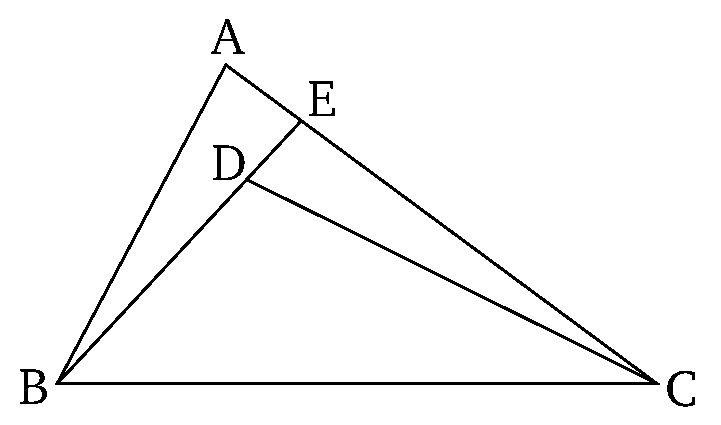
\includegraphics[width=0.5\linewidth]{figures/fig21e.eps}
    \label{fig:prop_21}
    \end{center}
\end{figure*}

If two internal straight-lines are constructed on one of the sides
of a triangle, from its ends, 
the constructed (straight-lines) will be less than the two remaining 
sides of the triangle, but will encompass a greater angle.

For let the two internal straight-lines $BD$ and $DC$ have been constructed on one of the sides $BC$ of the triangle $ABC$, from its ends $B$ and $C$ (respectively). I say that 
$BD$ and $DC$ are less than the (sum of the) two  remaining sides of the triangle
$BA$ and $AC$, but encompass an angle $BDC$ greater than $BAC$.

For let $BD$ have been drawn through to $E$. And since in any
triangle (the sum of any) two sides is greater than the remaining (side) [Prop.~1.20],
 in triangle $ABE$ the  (sum of the) two sides $AB$ and $AE$ is thus  greater than
$BE$. Let $EC$ have been added to both. Thus, (the sum of) $BA$ and $AC$ is greater
than (the sum of) $BE$ and $EC$.  Again, since in triangle $CED$ the (sum of the) two sides $CE$ and $ED$
is  greater than $CD$, let $DB$ have been added to both. Thus, 
(the sum of) $CE$ and $EB$ is greater than  (the sum of) $CD$ and $DB$. But, (the sum of) $BA$ and $AC$ was shown
(to be) greater than (the sum of) $BE$
 and $EC$. Thus, (the sum of) $BA$ and $AC$ is much greater than
(the sum of) $BD$ and $DC$.

Again, since in any  triangle the external angle 
is greater than the internal and opposite (angles) [Prop. 1.16],
 in triangle $CDE$ the external angle $BDC$ is thus greater
than $CED$.  Accordingly, for the same (reason),  the external angle $CEB$ of the
triangle $ABE$ is also greater than $BAC$. But, $BDC$ was shown (to be) 
greater
than $CEB$. Thus, $BDC$ is much greater than $BAC$.

Thus, if two internal straight-lines are constructed on one of the sides
of a triangle, from its ends, 
the constructed (straight-lines) are less than the two remaining 
sides of the triangle, but  encompass a greater angle. (Which is) the
very thing it was required to show.


\section*{Commentary}

\begin{proposition}\label{proposition_21}\lean{Elements.Book1.proposition_21}\leanok
    $D$ is a point inside $\triangle~ABC$. We have $|BD| + |DC|~<~|BA| + |AC|$, and $\angle~BDC~>~\angle~BAC$
\end{proposition}
\begin{proof}
    \uses{proposition_16,proposition_20}\leanok
    See the original proof by Euclid.
\end{proof}

\chapter*{Proposition 22}
\label{prop:22}

\begin{figure*}[ht]
    \begin{center}
    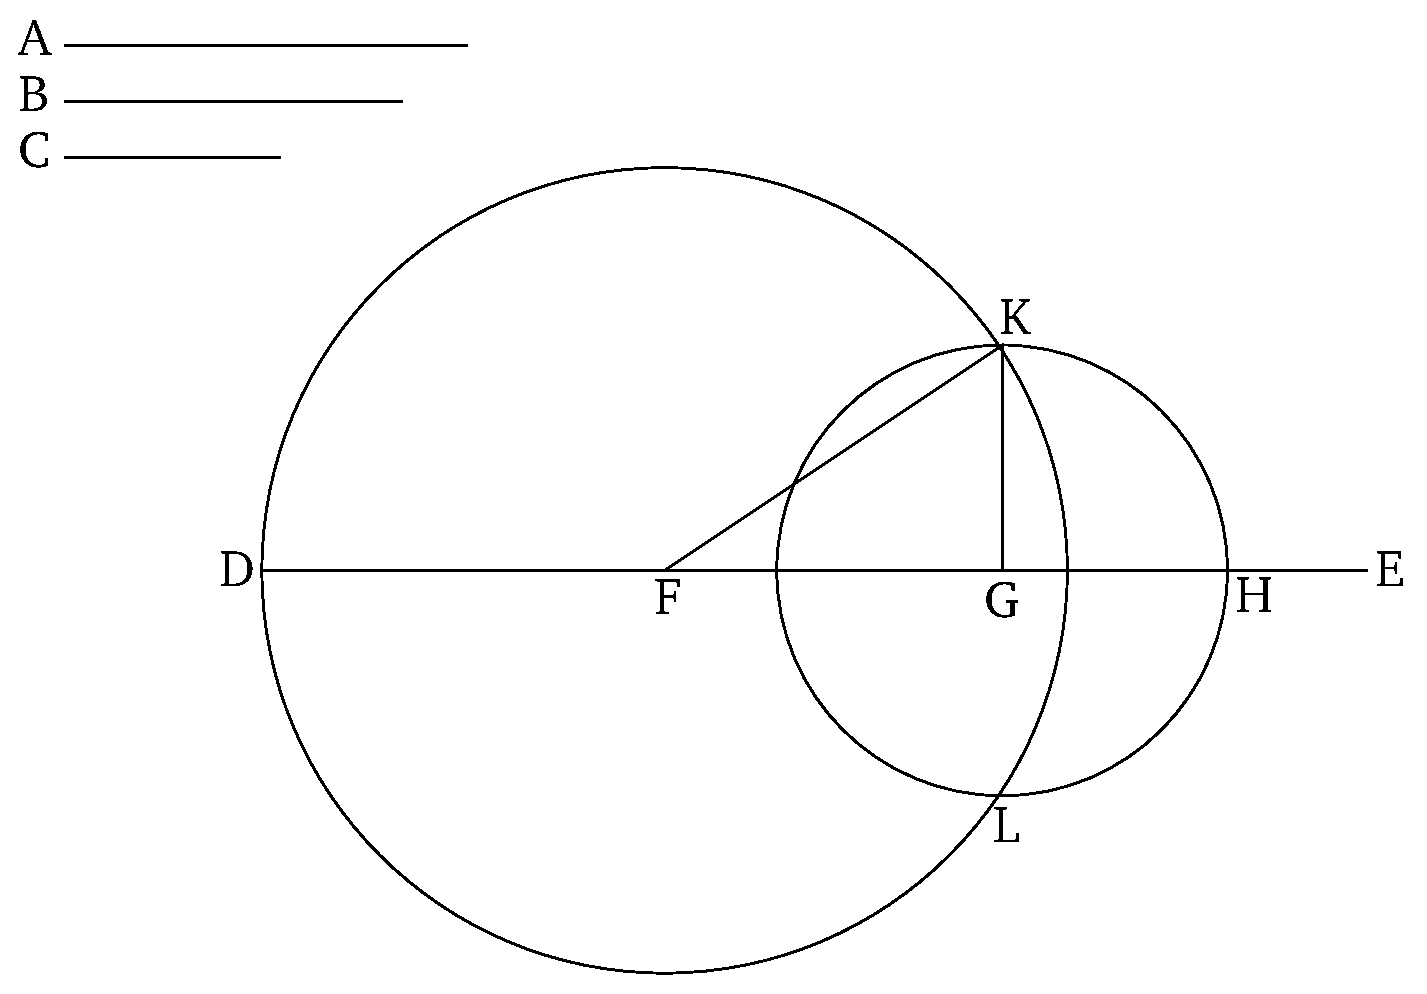
\includegraphics[width=0.5\linewidth]{figures/fig22e.eps}
    \label{fig:prop_22}
    \end{center}
\end{figure*}

To construct a triangle from three straight-lines which are equal to three given [straight-lines]. It is necessary for (the sum of) two (of the straight-lines) taken together in any (possible way) to be greater than the remaining (one), [on account of the (fact that)
 in any triangle (the sum of) two sides taken together in any (possible way) is greater than the remaining (one) [Prop.~1.20]\,].

Let $A$, $B$, and $C$ be the three given straight-lines, of which let (the sum of) two taken together in any (possible way)
be greater than the remaining (one). (Thus), (the sum of) $A$ and $B$ (is greater) than $C$, (the sum of) $A$ and $C$ than $B$,
and also (the sum of) $B$ and $C$ than $A$. So it is required to construct a triangle
from (straight-lines) equal to $A$, $B$, and $C$.

Let some straight-line $DE$ be set out, terminated at $D$, and infinite in the
direction of $E$.  And let $DF$ made equal to $A$, and $FG$
equal to $B$, and $GH$ equal to $C$ [Prop.~1.3]. And let the
circle $DKL$ have been drawn with center $F$ and radius $FD$. Again,
let the circle $KLH$ have been drawn with center $G$ and radius $GH$. And
let $KF$ and $KG$ have been joined. I say that the triangle $KFG$ has been
constructed from three straight-lines equal to $A$, $B$, and $C$.

For since point $F$ is the center of the circle $DKL$, $FD$ is equal to $FK$.
But, $FD$ is equal to $A$. Thus, $KF$ is also equal to $A$. Again, since point
$G$ is the center of the circle $LKH$, $GH$ is equal to $GK$. But, $GH$ is equal
to $C$. Thus, $KG$ is also equal to $C$. And $FG$ is also equal to $B$. Thus,
the three straight-lines $KF$, $FG$, and $GK$ are equal to $A$, $B$, and $C$ (respectively).

Thus, the triangle $KFG$ has been constructed from the three straight-lines
$KF$, $FG$, and $GK$, which are equal to the three given straight-lines
$A$, $B$, and $C$ (respectively). (Which is) the very thing it was required
to do.


\section*{Commentary}

\begin{proposition}\label{proposition_22}\lean{Elements.Book1.proposition_22}\leanok
    $A$ and $A'$ are two disctinct points on a line $AA'$. $B$ and $B'$ are two distinct points on a line $BB'$. $C$ and $C'$ are two distinct points on a line $CC'$. $|AA'| + |BB'|~>~|CC'|$, $|AA'| + |CC'|~>~|BB'|$, and $|BB'| + |CC'|~>~|AA'|$. Then, there must exist $\triangle~KFG$, s.t., $|FK| = |AA'|$, $|FG| = |BB'|$, and $|KG| = |CC'|$.
\end{proposition}
\begin{proof}
    \uses{proposition_3}\leanok
    See the original proof by Euclid.
\end{proof}


Euclid only proved that $\triangle~KFG$ can be constructed. However, in later proofs, we need $\triangle~KFG$ to be constructed on a given line and a given side of the line.

\begin{proposition}\label{proposition_22'}\lean{Elements.Book1.proposition_22'}\leanok
    $A$ and $A'$ are two disctinct points on a line $AA'$. $B$ and $B'$ are two distinct points on a line $BB'$. $C$ and $C'$ are two distinct points on a line $CC'$. $F$ and $E$ are two distinct points on a line $FE$. $|AA'| + |BB'|~>~|CC'|$, $|AA'| + |CC'|~>~|BB'|$, and $|BB'| + |CC'|~>~|AA'|$. Then, there must exist $\triangle~KFG$, s.t., $G$ and $F$ are on $FE$, $F$ not between $G$ and $E$, $|FK| = |AA'|$, $|FG| = |BB'|$, and $|KG| = |CC'|$.
\end{proposition}
\begin{proof}
    \uses{proposition_3}\leanok
    The same proof as Euclid's.
\end{proof}

\begin{proposition}\label{proposition_22''}\lean{Elements.Book1.proposition_22''}\leanok
    $A$ and $A'$ are two disctinct points on a line $AA'$. $B$ and $B'$ are two distinct points on a line $BB'$. $C$ and $C'$ are two distinct points on a line $CC'$. $F$ and $E$ are two distinct points on a line $FE$. $X$ is a point not on $FE$. $|AA'| + |BB'|~>~|CC'|$, $|AA'| + |CC'|~>~|BB'|$, and $|BB'| + |CC'|~>~|AA'|$. Then, there must exist $\triangle~KFG$, s.t., $G$ and $F$ are on $FE$, $F$ not between $G$ and $E$, $K$ on the same side of $FE$ with $X$, $|FK| = |AA'|$, $|FG| = |BB'|$, and $|KG| = |CC'|$.
\end{proposition}
\begin{proof}
    \uses{proposition_3}\leanok
    The same proof as Euclid's.
\end{proof}
\chapter*{Proposition 23}
\label{prop:23}

\begin{figure*}[ht]
    \begin{center}
    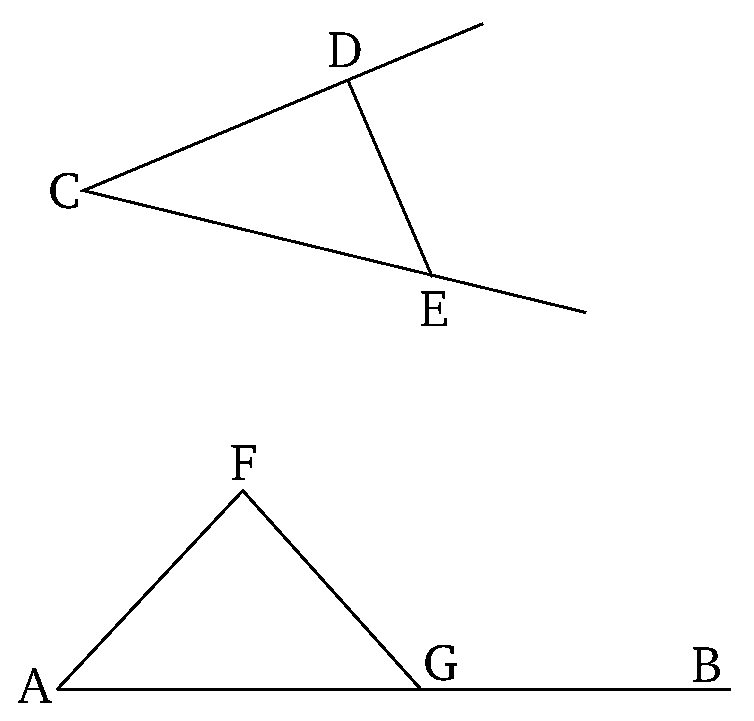
\includegraphics[width=0.5\linewidth]{figures/fig23e.eps}
    \label{fig:prop_23}
    \end{center}
\end{figure*}

To construct a rectilinear angle equal to a given rectilinear angle at a (given)
point on a given straight-line.\\

Let $AB$ be the given straight-line,  $A$ the (given) point on it, and 
$DCE$ the given rectilinear angle. So it is required to construct a rectilinear
angle equal to the given rectilinear angle $DCE$ at the (given) point
$A$ on the given straight-line
$AB$.

Let the points $D$ and $E$ have been taken at random on each
of the (straight-lines) $CD$ and $CE$ (respectively), and let $DE$ have been joined.
And let the triangle $AFG$ have been constructed from three straight-lines
which are equal to $CD$, $DE$, and $CE$, such that $CD$ is equal to $AF$,
$CE$ to $AG$, and further $DE$ to $FG$ [Prop.~1.22].

Therefore, since the two (straight-lines) $DC$, $CE$ are equal to the
two (straight-lines) $FA$, $AG$, respectively, and the base $DE$ is equal to
the base $FG$, the angle $DCE$ is thus equal to the angle $FAG$ [Prop.~1.8].

Thus, the rectilinear angle $FAG$,  equal to the  given
rectilinear angle $DCE$, has been constructed at the (given) point $A$ on the given straight-line $AB$.
(Which is) the very thing it was required to do.


\section*{Commentary}

\begin{proposition}\label{proposition_23}\lean{Elements.Book1.proposition_23}\leanok
    $\angle~DCE$ is an angle. $A$ and $B$ are two distinct points on a line $AB$. Then, there must exists a point $F$ different from $A$, s.t., $\angle~FAB = \angle~DCE$.
\end{proposition}
\begin{proof}
    \uses{proposition_8,proposition_20,proposition_22'}\leanok
    Euclid's proof omitted the degenerated cases that $D$ is on $CE$, i.e., $\angle~DCE$ is either $0$ or $\pi$.
    In addition, when constructing $\triangle~AFG$, Euclid didn't prove that such a triangle can be constructed from $CD$, $CE$, and $DE$, which can be done by applying Proposition~\ref{proposition_20}.
\end{proof}

Euclid didn't prove that $F$ can be constructed on either side of $AB$, which is useful for later proofs.

\begin{proposition}\label{proposition_23'}\lean{Elements.Book1.proposition_23'}\leanok
    $\angle~DCE$ is an angle. $A$ and $B$ are two distinct points on a line $AB$. $X$ is a point not on $AB$. Then, there must exists a point $F$ different from $A$, s.t., $\angle~FAB = \angle~DCE$, and $F$ is either on $AB$ or on the same side of $AB$ with $X$.
\end{proposition}
\begin{proof}
    \uses{proposition_8,proposition_20,proposition_22''}\leanok
    Similar to the previous proof.
\end{proof}
\chapter*{Proposition 24}
\label{prop:24}

\begin{figure*}[ht]
    \begin{center}
    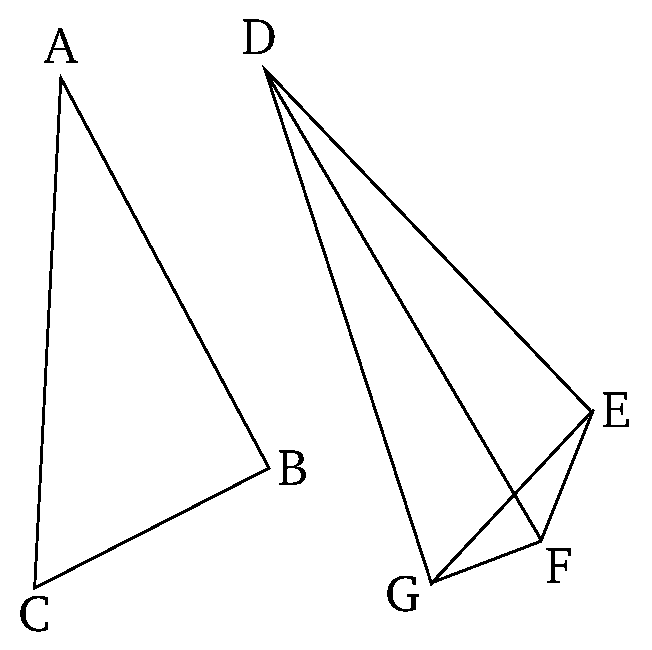
\includegraphics[width=0.5\linewidth]{figures/fig24e.eps}
    \label{fig:prop_24}
    \end{center}
\end{figure*}

If two triangles have two sides equal to two sides, respectively,
but (one) has the angle encompassed by the equal straight-lines greater than the (corresponding)
angle (in the other), then (the former triangle) will also have a base greater than the base (of the latter).

Let  $ABC$ and $DEF$ be two triangles having the two sides $AB$ and $AC$
equal to the two sides $DE$ and $DF$, respectively. (That is), $AB$ (equal) to $DE$, and
$AC$ to $DF$.  Let them also have the angle at $A$ greater than the angle at $D$.
I say that the base $BC$ is also greater than the base $EF$.

For since angle $BAC$ is greater than angle $EDF$, let (angle) $EDG$, equal to
angle $BAC$,  have been constructed at  the point $D$ on the straight-line $DE$ [Prop.~1.23]. And let $DG$ be made equal to either of $AC$ or $DF$ [Prop.~1.3], and let $EG$ and $FG$ have been joined.

Therefore, since $AB$ is equal to $DE$ and $AC$ to $DG$, the two (straight-lines)
$BA$, $AC$ are equal to the two (straight-lines) $ED$, $DG$, respectively.
Also the angle $BAC$ is equal to the angle $EDG$. Thus, the base $BC$ is equal
to the base $EG$ [Prop.~1.4]. Again, since $DF$ is equal to $DG$, angle $DGF$
is also equal to angle $DFG$ [Prop.~1.5]. Thus, $DFG$ (is) greater than $EGF$.
Thus, $EFG$ is much greater than $EGF$. And since triangle $EFG$ has angle $EFG$
greater than $EGF$, and the greater angle is subtended by the greater side [Prop.~1.19], side $EG$ (is) thus also greater than $EF$. But $EG$ (is) equal to
$BC$. Thus, $BC$ (is) also greater than $EF$.

Thus, if two triangles have two sides equal to two sides, respectively,
but (one) has the angle encompassed by the equal straight-lines greater than the 
(corresponding) angle (in the other), then (the former triangle) will also have a base greater than the base (of the latter).
(Which is) the very thing it was required to show.


\section*{Commentary}

Euclid did not cover the case where $D$ and $G$ are on different sides of $EF$ (Fig.~\ref{fig:prop_24b}). Below we augment Euclid's proof to cover this case. The resulting proof is significantly more complicated than Euclid's proof.

\begin{figure*}[ht]
    \begin{center}
    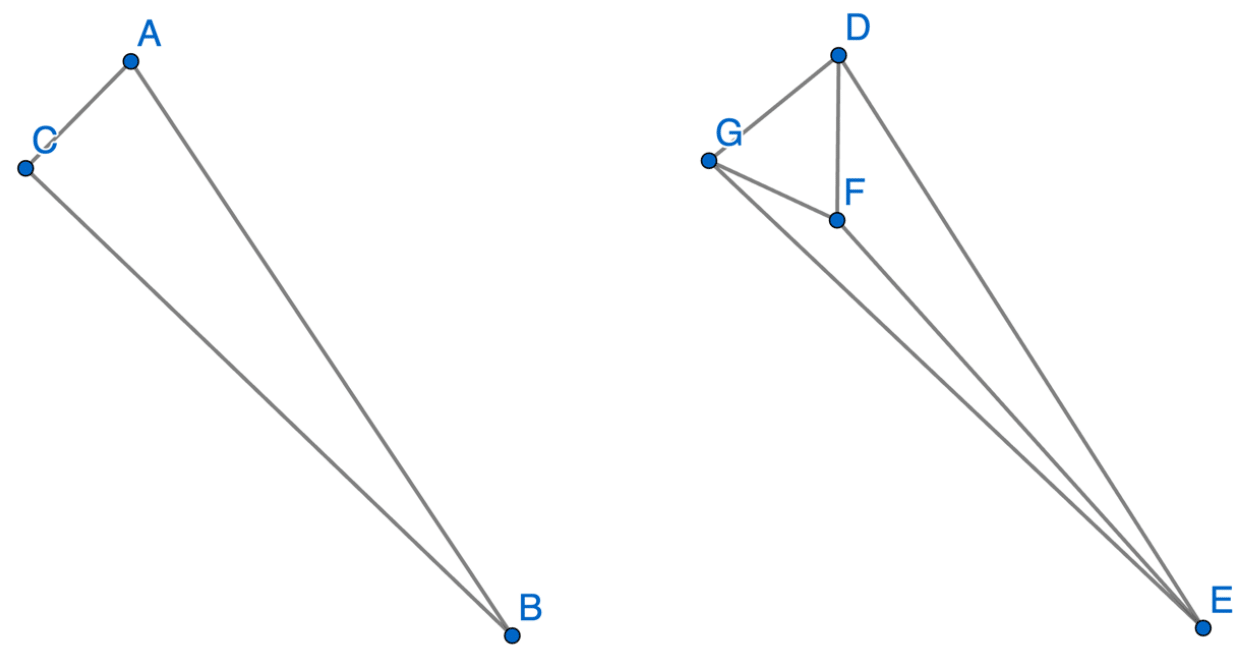
\includegraphics[width=0.35\linewidth]{figures/proposition_24.png}
    \caption{The case in Proposition~24 missed by Euclid.}
    \label{fig:prop_24b}
    \end{center}
\end{figure*}


\begin{proposition}\label{proposition_24}\lean{Elements.Book1.proposition_24}\leanok
    $\triangle~ABC$ and $\triangle~DEF$ are two triangles s.t., $|AB|=|DE|$, $|AC|=|DF|$, and $\angle~BAC~>~\angle~EDF$. Then, $|BC|~>~|EF|$.
\end{proposition}
\begin{proof}
    \uses{proposition_3,proposition_4,proposition_5,proposition_13,proposition_17,proposition_19,proposition_23}\leanok
    We only prove the case missed by Euclid. 
    
    Let's construct $\triangle~EDG$ s.t., $\angle~EDG = \angle~BAC$, $|DG|=|DF|$, and $|BC|=|EG|$ (Fig.~\ref{fig:prop_24b}). By Proposition~5, we have $\angle~DGF = \angle~DFG$; let's denote it by $\alpha$. To prove $|BC|~>~|EF|$, we only need to prove $|EG|~>~|EF|$. By Proposition~19, this is further reduced to $\angle~EFG~>~\angle~EGF$. Let $x = \angle~EFG$ and $y = \angle~EGF$. We want to prove $x~>~y$.
    
    Note that $\angle~DGE = \angle~DGF + \angle~EGF = \alpha + y$. $\angle~DFE = 2\pi - \angle~DFG - \angle~EFG = 2\pi - \alpha - x$. Furthermore, Proposition~17 states that the sum of any two angles in a triangle must be smaller than $\pi$. Therefore, any angle in a triangle must also be smaller than $\pi$, i.e.,
    \begin{eqnarray*}
        \alpha + y &~<~& \pi \\
        2\pi - \alpha - x &~<~& \pi
    \end{eqnarray*}
    Simplifying these two inequalities leads to $x~>~y$. QED.

\end{proof}

\chapter*{Proposition 25}



\begin{figure*}[ht]
    \begin{center}
    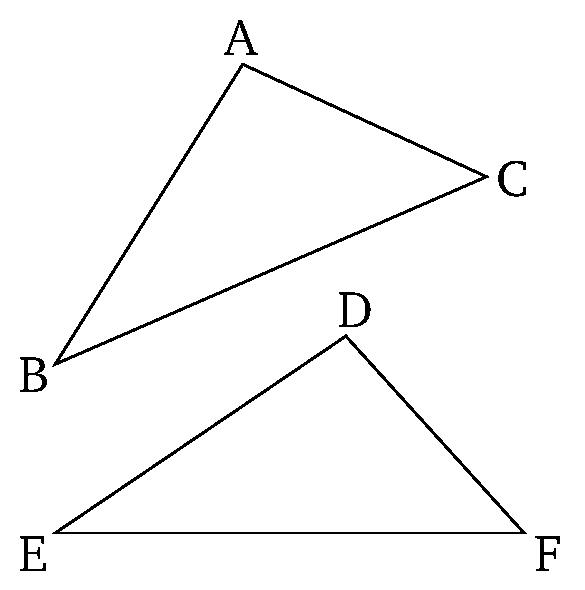
\includegraphics[width=0.5\linewidth]{figures/fig25e.eps}
    \label{fig:prop_25}
    \end{center}
\end{figure*}

If two triangles have two sides equal to two sides, respectively,
but (one) has a base greater than the base (of the other), then (the former triangle) will also have the angle encompassed by the equal straight-lines greater than the (corresponding) angle (in the latter).

Let $ABC$ and $DEF$ be  two triangles having the two sides $AB$ and $AC$
equal to the two sides $DE$ and $DF$, respectively (That is), $AB$ (equal) to $DE$, and $AC$ to $DF$. And let the base $BC$ be greater than the base $EF$. I say that angle
$BAC$ is also greater than $EDF$.

For if not, ($BAC$) is certainly either equal to, or less than, ($EDF$). In fact, $BAC$ is not equal to
$EDF$. For then the base $BC$ would also have been equal to the base $EF$ [Prop.~1.4]. But it is not.
Thus, angle $BAC$ is not equal to $EDF$. Neither, indeed, is $BAC$ less
than $EDF$. For then the base $BC$ would also have been less than the base $EF$ [Prop.~1.24].
But it is not. Thus, angle $BAC$ is not less than $EDF$. But it was  shown
that ($BAC$ is) not equal (to $EDF$) either. Thus, $BAC$ is greater than $EDF$.

Thus, if two triangles have two sides equal to two sides, respectively,
but (one) has a base greater than the base (of the other), then (the former triangle) will also have the angle encompassed by the equal straight-lines greater than the (corresponding) angle (in the latter). (Which is) the
very thing it was required to show.


\section*{Commentary}

\begin{proposition}\label{proposition_25}\lean{Elements.Book1.proposition_25}\leanok
    $\triangle~ABC$ and $\triangle~DEF$ are two triangles s.t. $|AB|=|DE|$, $|AC|=|DF|$, and $|BC|~>~|EF|$. Then, $\angle~BAC~>~\angle~EDF$.
\end{proposition}
\begin{proof}
    \uses{proposition_4,proposition_24}\leanok
    See the original proof by Euclid.
\end{proof}

\chapter*{Proposition 26}

\begin{figure*}[ht]
    \begin{center}
    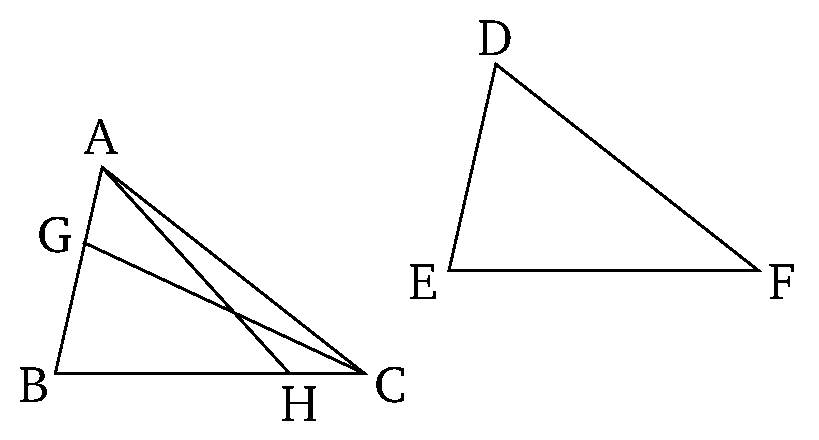
\includegraphics[width=0.5\linewidth]{figures/fig26e.eps}
    \label{fig:prop_26}
    \end{center}
\end{figure*}


If  two triangles have two angles equal to two angles, respectively, 
and one side equal to one side---in fact, either that by the equal angles, or that
subtending one of the equal angles---then (the triangles) will also have the remaining
sides equal to the [corresponding] remaining sides, and the
remaining angle (equal) to the remaining angle.

Let $ABC$ and $DEF$ be two triangles having the two angles $ABC$ and
$BCA$ equal to the two (angles) $DEF$ and $EFD$, respectively.
(That is) $ABC$ (equal) to $DEF$, and $BCA$ to $EFD$. And let them also have
one side equal to one side. First of all, the (side) by the equal angles. (That is)
$BC$ (equal) to $EF$. I say that they will have the  remaining sides equal to the
corresponding remaining sides. (That is) $AB$ (equal) to $DE$, and $AC$ to
$DF$. And (they will have) the remaining angle (equal) to the remaining angle.
(That is) $BAC$ (equal) to $EDF$.

For if $AB$ is unequal to $DE$ then one of them is greater. Let $AB$ be greater,
and let $BG$ be made equal to $DE$ [Prop.~1.3], and let $GC$ have been
joined.

Therefore, since $BG$ is equal to $DE$, and $BC$ to $EF$, the two (straight-lines)
$GB$, $BC$ are equal to the two (straight-lines) $DE$, $EF$, respectively. And angle
$GBC$ is equal to angle $DEF$. Thus, the base $GC$ is equal to the base $DF$,
and triangle $GBC$ is equal to triangle $DEF$, and the remaining angles 
subtended by the equal sides will
be equal to the (corresponding) remaining angles [Prop.~1.4].
Thus, $GCB$ (is equal) to $DFE$. But,  $DFE$ was assumed (to be) equal to $BCA$.
Thus, $BCG$ is also equal to $BCA$, the lesser to the greater. The very thing (is) impossible. Thus, $AB$ is not unequal to $DE$. Thus, (it is) equal. And $BC$ is
also equal to $EF$. So the two (straight-lines) $AB$, $BC$ are equal to the two (straight-lines) $DE$, $EF$, respectively. And angle $ABC$ is equal to
angle $DEF$. Thus, the base $AC$ is equal to the base $DF$, and the remaining
angle $BAC$ is equal to the remaining angle $EDF$ [Prop.~1.4].

But, again, let the sides subtending the equal angles be equal: for instance, 
(let) $AB$ (be equal) to
$DE$.  Again, I say that the remaining sides will be equal to the remaining
sides. (That is) $AC$ (equal) to $DF$, and $BC$ to $EF$. Furthermore, the remaining angle
$BAC$ is equal to the remaining angle $EDF$.

For if $BC$ is unequal to $EF$ then one of them is greater. If possible, let $BC$
be greater. And let $BH$ be made equal to $EF$ [Prop.~1.3], and let $AH$ have been joined.
And since $BH$ is equal to $EF$, and $AB$ to $DE$, the two (straight-lines) $AB$, $BH$
are equal to the two (straight-lines) $DE$, $EF$, respectively. And the angles
they encompass (are also equal). Thus, the base $AH$ is equal to the base  
$DF$, and the triangle $ABH$ is equal to the triangle $DEF$, and the
remaining angles subtended by the equal sides will be equal to the
(corresponding) remaining angles [Prop.~1.4]. Thus, angle $BHA$ 
is equal to $EFD$. But, $EFD$ is equal to $BCA$. So, in triangle $AHC$,
the external angle $BHA$ is equal to the internal and opposite angle 
$BCA$. The very thing (is) impossible [Prop.~1.16]. Thus, $BC$ is not unequal to $EF$.
Thus, (it is) equal. And $AB$ is also equal to $DE$. So the two
(straight-lines) $AB$, $BC$ are equal to the two (straight-lines) $DE$, $EF$,
respectively. And they encompass equal angles. Thus, the base $AC$ is equal
to the base $DF$, and triangle $ABC$ (is) equal to triangle $DEF$, and the
remaining angle $BAC$ (is) equal to the remaining angle $EDF$ [Prop.~1.4].

Thus, if two triangles have two angles equal to two angles, respectively, 
and one side equal to one side---in fact, either that by the equal angles, or that
subtending one of the equal angles---then (the triangles) will also have the remaining sides equal to the (corresponding) remaining sides, and the
remaining angle (equal) to the remaining angle. (Which is) the very thing it
was required to show.



\section*{Commentary}

\begin{proposition}\label{proposition_26}\lean{Elements.Book1.proposition_26}\leanok
    $\triangle~ABC$ and $\triangle~DEF$ are two triangles, s.t., $\angle~ABC=\angle~DEF$, $\angle~BCA=\angle~EFD$, and $|BC|=|EF|$ (or $|AB|=|DE|$). Then, $\triangle~ABC\cong\triangle~DEF$.
\end{proposition}
\begin{proof}
    \uses{proposition_3,proposition_4,proposition_16}\leanok
    See the original proof by Euclid.
\end{proof}

\chapter*{Proposition 27}

\begin{figure*}[ht]
    \begin{center}
    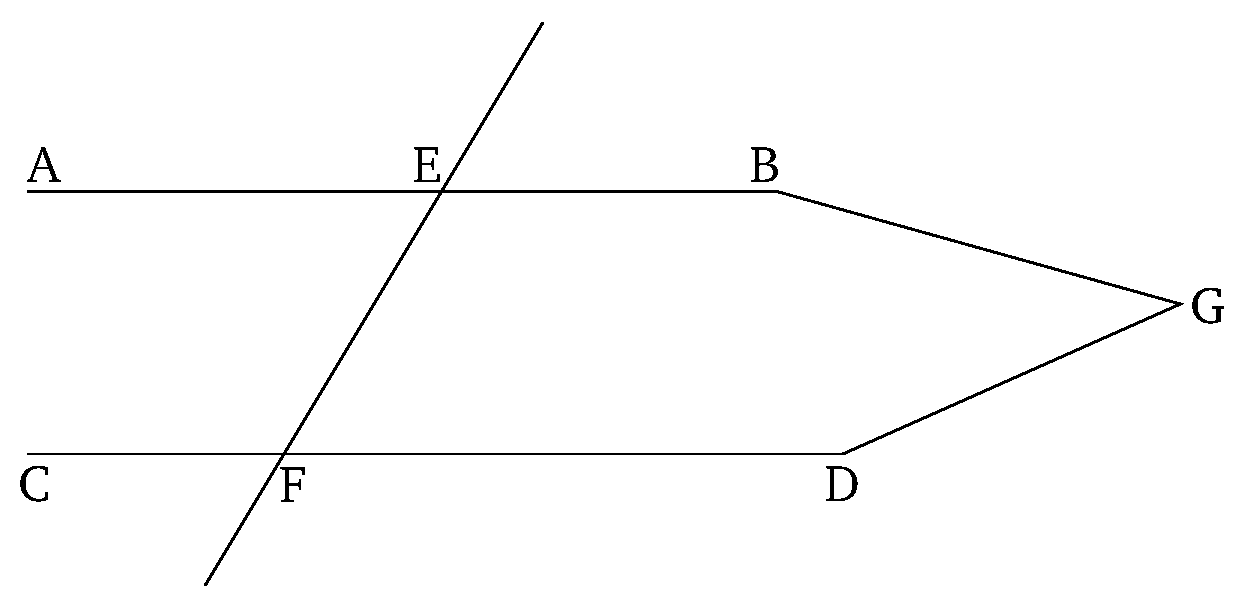
\includegraphics[width=0.5\linewidth]{figures/fig27e.eps}
    \label{fig:prop_27}
    \end{center}
\end{figure*}

If a straight-line falling across two straight-lines makes  the alternate
angles equal to one another then the (two) straight-lines will be parallel to
one another.

For let the straight-line $EF$, falling across the two straight-lines $AB$ and
$CD$, make the alternate angles $AEF$ and $EFD$ equal to one another.
I say that $AB$ and $CD$ are parallel.

For if not, being produced, $AB$ and $CD$ will certainly meet together:
either in the direction of $B$ and $D$, or (in the
direction) of $A$ and $C$ [Def.~\ref{def:23}]. Let them have been
produced, and let them meet together in the direction of $B$ and $D$ at
 (point) $G$. So, for the triangle $GEF$, the external angle
$AEF$ is equal to the interior and opposite (angle) $EFG$. The
very thing is impossible [Prop.~1.16]. Thus, being produced, $AB$ and $CD$
will not meet together in the direction of $B$ and $D$. Similarly, 
it can be shown that neither (will they meet together) in (the
direction of) $A$ and $C$. But  (straight-lines) meeting in neither
direction are parallel [Def.~\ref{def:23}]. Thus, $AB$ and $CD$ are parallel.

Thus, if a straight-line falling across two straight-lines makes  the alternate
angles equal to one another then the (two) straight-lines will be parallel (to
one another). (Which is) the very thing it was required to show.


\section*{Commentary}

\begin{proposition}\label{proposition_27}\lean{Elements.Book1.proposition_27}\leanok
    $A$ and $E$ are two distcint points on the line $AE$. $F$ and $D$ are two distinct points on $FD$. $E$ and $F$ are two distinct points on $EF$. $A$ and $D$ are on different sides of $EF$. $\angle~AEF = \angle~EFD$. Then, $AE$ and $FD$ must be parallel.
\end{proposition}
\begin{proof}
    \uses{proposition_16}\leanok
    See the original proof by Euclid.
\end{proof}


\chapter*{Proposition 28}



\begin{figure*}[ht]
    \begin{center}
    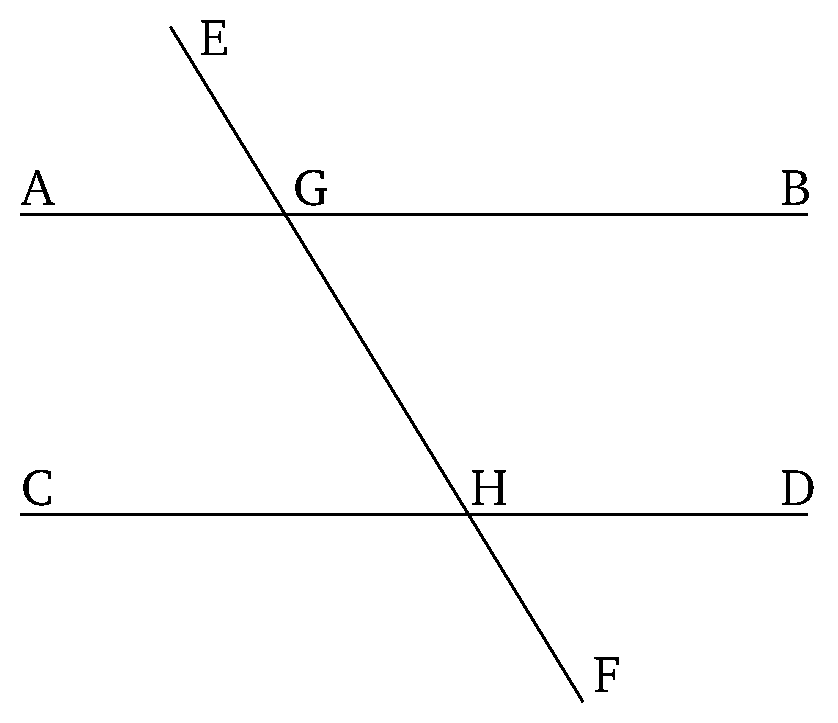
\includegraphics[width=0.5\linewidth]{figures/fig28e.eps}
    \label{fig:prop_28}
    \end{center}
\end{figure*}

If a straight-line falling across two straight-lines makes the external angle equal
to the internal and opposite angle on the same side, or (makes) the (sum  of the) internal
(angles) on the same side equal
to two right-angles, then the (two) straight-lines will be parallel to
one another.

For let $EF$, falling across the two straight-lines $AB$ and $CD$, make the external
angle $EGB$ equal to the internal and opposite angle $GHD$, or the (sum of the) internal
(angles) on the same side, $BGH$ and $GHD$, equal to two right-angles.
I say that $AB$ is parallel to $CD$.

For since (in the first case) $EGB$ is equal to $GHD$, but $EGB$ is equal to $AGH$ [Prop.~1.15],
$AGH$ is thus also equal to $GHD$. And they are alternate (angles).
Thus, $AB$ is
 parallel to $CD$ [Prop.~1.27].
 
Again, since (in the second case, the sum of) $BGH$ and $GHD$ is equal to two right-angles,  and (the sum of) $AGH$ and
$BGH$ is also equal to two right-angles [Prop.~1.13], 
(the sum of) $AGH$ and $BGH$ is thus equal to (the sum of) $BGH$ and $GHD$. Let $BGH$ have been
subtracted from both. Thus, the remainder $AGH$ is equal to the remainder
$GHD$. And they are alternate (angles). Thus, $AB$ is parallel
to $CD$ [Prop.~1.27].

Thus, if a straight-line falling across  two straight-lines makes the external angle equal
to the internal and opposite angle on the same side, or (makes) the (sum of the) internal
(angles) on the same side equal
to two right-angles, then the (two) straight-lines will be parallel (to
one another). (Which is) the very thing it was required to show.


\section*{Commentary}

\begin{proposition}\label{proposition_28}\lean{Elements.Book1.proposition_28}\leanok
    $A$ and $B$ are two distcint points on $AB$. $C$ and $D$ are two distinct points on $CD$. $E$ and $F$ are two distinct points on $EF$. $G$ is between $A$ and $B$. $H$ is between $C$ and $D$. $G$ is between $E$ and $H$. $H$ is between $G$ and $F$. $B$ and $D$ are on the same side of $EF$. Either $\angle~EGB = \angle~GHD$ or $\angle~BGH + \angle~GHD = \pi$. Then, $AB$ and $CD$ must be parallel.
\end{proposition}
\begin{proof}
    \uses{proposition_13,proposition_15,proposition_27}\leanok
    See the original proof by Euclid.
\end{proof}

\chapter*{Proposition 29}


\begin{figure*}[ht]
    \begin{center}
    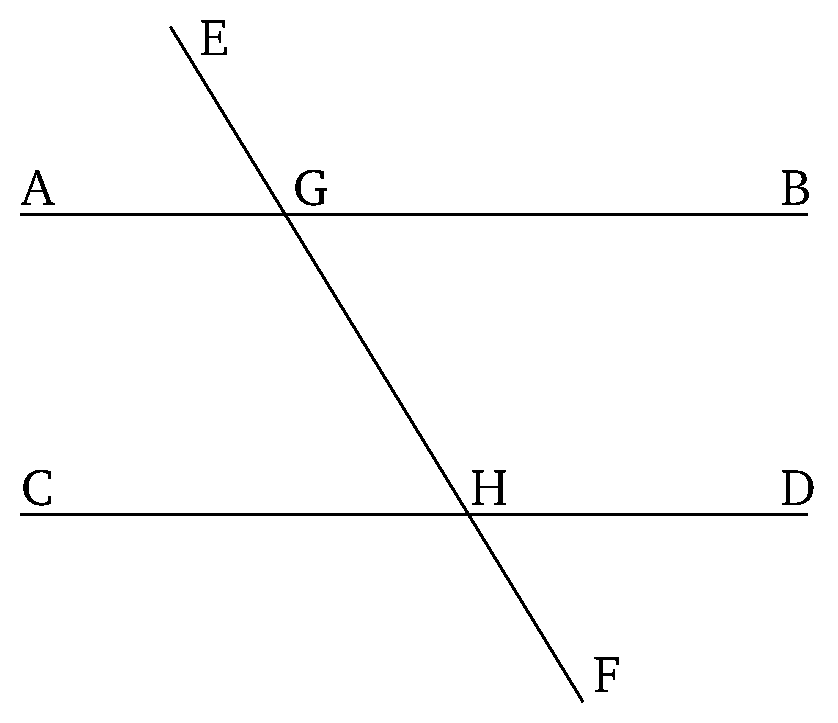
\includegraphics[width=0.5\linewidth]{figures/fig28e.eps}
    \label{fig:prop_29}
    \end{center}
\end{figure*}

A straight-line falling across  parallel straight-lines makes the alternate angles
equal to one another,  the external (angle) equal to the internal and
opposite (angle), and the (sum of the) internal (angles) on the same side equal to
two right-angles.

For let the straight-line $EF$ fall across the parallel straight-lines $AB$ and $CD$.
I say that it makes the  alternate angles, $AGH$ and $GHD$,  equal,  the
external angle $EGB$ equal to the internal and opposite (angle) $GHD$,
and the (sum of the) internal (angles) on the same side, $BGH$ and $GHD$, equal to
two right-angles.

For if $AGH$ is unequal to $GHD$ then one of them is greater. Let $AGH$ be greater.
Let $BGH$ have been added to both. Thus, (the sum of) $AGH$ and $BGH$ is greater
than (the sum of) $BGH$ and $GHD$. But, (the sum of) $AGH$ and $BGH$ is equal to two right-angles
[Prop~1.13]. Thus,  (the sum of) $BGH$ and $GHD$ is [also] less than two right-angles. 
But (straight-lines) being produced to infinity from (internal angles whose sum is) less than
two right-angles meet together [Post.~\ref{post:5}]. Thus, $AB$ and $CD$, being produced to
infinity, will meet together. But they do not meet, on account of
them (initially) being assumed parallel (to one another) [Def.~\ref{def:23}]. Thus, $AGH$ is not unequal to $GHD$. Thus, (it is) equal. But, $AGH$ is equal to $EGB$ [Prop.~1.15]. 
And $EGB$ is thus also equal to $GHD$.
Let $BGH$
be added to both. Thus, (the sum of) $EGB$ and $BGH$ is equal to (the sum of) $BGH$ and $GHD$.
But, (the sum of) $EGB$ and $BGH$ is equal to two right-angles [Prop.~1.13]. 
Thus, (the sum of) $BGH$ and $GHD$ is also equal to two right-angles.

Thus, a straight-line falling across parallel straight-lines makes the alternate angles
equal to one another,  the external (angle) equal to the internal and
opposite (angle), and the (sum of the) internal (angles) on the same side equal to
two right-angles. (Which is) the very thing it was required to show.


\section*{Commentary}

\begin{proposition}\label{proposition_29}\lean{Elements.Book1.proposition_29}\leanok
    If
\end{proposition}
\begin{proof}
    \uses{proposition_13,proposition_15}\leanok
\end{proof}

\chapter*{Proposition 30}



\begin{figure*}[ht]
    \begin{center}
    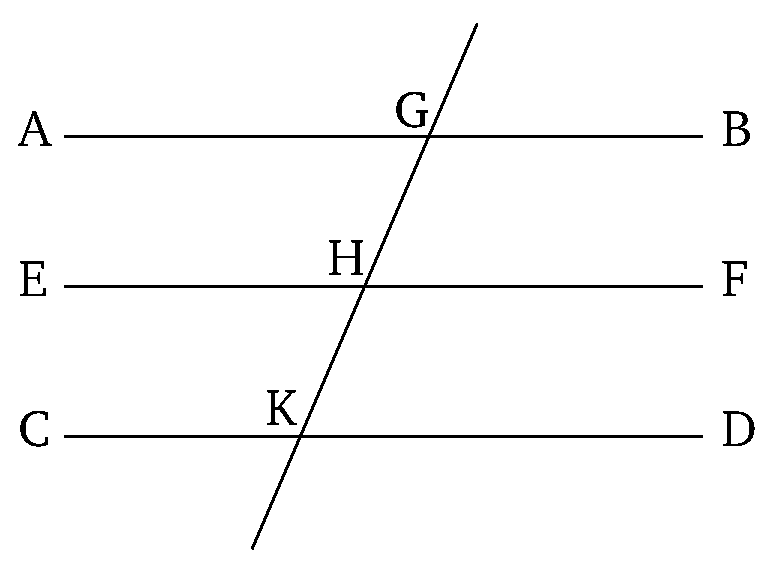
\includegraphics[width=0.5\linewidth]{figures/fig30e.eps}
    \label{fig:prop_30}
    \end{center}
\end{figure*}

(Straight-lines) parallel to the same straight-line are also parallel
to one another.

Let each of the (straight-lines) $AB$ and $CD$ be parallel to $EF$. I say that
$AB$ is also parallel to $CD$.

For let the straight-line $GK$ fall across  ($AB$, $CD$, and $EF$).

And since the straight-line $GK$ has fallen across the parallel straight-lines $AB$ and $EF$, (angle) $AGK$
(is) thus equal to $GHF$ [Prop.~1.29]. Again, since the straight-line $GK$ has fallen across the parallel
straight-lines $EF$ and $CD$, (angle) $GHF$ is equal to $GKD$ [Prop.~1.29].
But $AGK$ was also shown (to be) equal to $GHF$. Thus, $AGK$ is also equal to 
$GKD$. And they are alternate (angles). Thus, $AB$ is parallel to $CD$ [Prop.~1.27].

\mbox{[}Thus, (straight-lines) parallel to the same straight-line are also parallel
to one another.] (Which is) the very thing it was required to show.


\section*{Commentary}

\begin{proposition}\label{proposition_30}\lean{Elements.Book1.proposition_30}\leanok
    If
\end{proposition}
\begin{proof}
    \uses{proposition_27,proposition_29}\leanok
\end{proof}

\chapter*{Proposition 31}



\begin{figure*}[ht]
    \begin{center}
    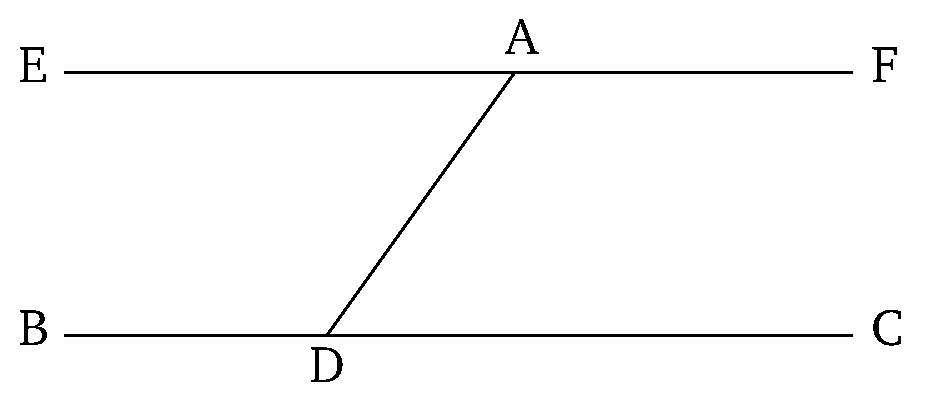
\includegraphics[width=0.5\linewidth]{figures/fig31e.eps}
    \label{fig:prop_31}
    \end{center}
\end{figure*}

To draw a straight-line parallel to a given straight-line, through a given
point.

Let $A$ be the given point, and $BC$ the given straight-line. So it is
required to draw a straight-line parallel to the straight-line $BC$, through
the point $A$.

Let the point $D$ have been taken a random  on $BC$, and let $AD$ have been
joined. And let (angle) $DAE$, equal to angle $ADC$,  have been constructed 
on the straight-line $DA$ at the point $A$ on it [Prop.~1.23]. And let the
straight-line $AF$ have been
produced in a straight-line with $EA$.

And since the straight-line $AD$, (in) falling across the two straight-lines
$BC$ and $EF$,  has made the alternate
angles $EAD$ and $ADC$ equal to one another, $EAF$ is thus parallel to $BC$
[Prop.~1.27].

Thus, the straight-line $EAF$ has been drawn parallel to the given straight-line $BC$, through the  given
point $A$. (Which is) the very thing it was required to do.


\section*{Commentary}

\begin{proposition}\label{proposition_31}\lean{Elements.Book1.proposition_31}\leanok
    If
\end{proposition}
\begin{proof}
    \uses{proposition_23,proposition_27}\leanok
\end{proof}

\chapter*{Proposition 32}



\begin{figure*}[ht]
    \begin{center}
    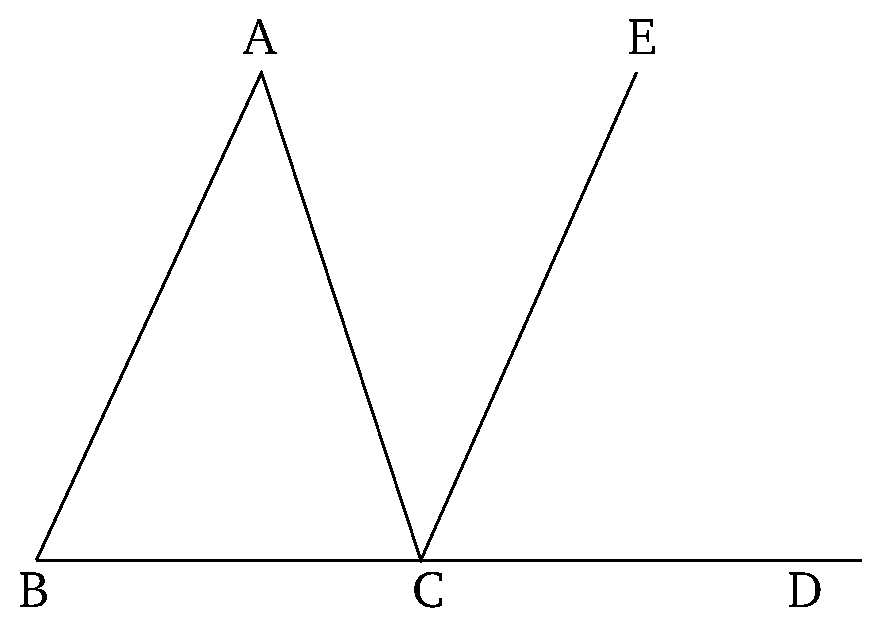
\includegraphics[width=0.5\linewidth]{figures/fig32e.eps}
    \label{fig:prop_32}
    \end{center}
\end{figure*}

In any triangle,  (if) one of the sides (is) produced  (then) the external
angle is equal to the (sum of the) two internal and opposite (angles), and the (sum of the) three
internal angles of the triangle is equal to two right-angles.

Let $ABC$ be a triangle, and let one of its sides $BC$ have been produced to $D$.
I say that the external angle $ACD$ is equal to the (sum of the) two internal and opposite
angles $CAB$ and $ABC$, and the (sum of the) three internal angles of the triangle---$ABC$, $BCA$, and $CAB$---is equal to two right-angles.

For let $CE$ have been drawn through point $C$ parallel to the straight-line
$AB$ [Prop.~1.31].

And since $AB$ is parallel to $CE$, and $AC$ has fallen across them, the alternate
angles $BAC$ and $ACE$ are equal to one another [Prop.~1.29]. Again,
since $AB$ is parallel to $CE$, and the straight-line $BD$ has fallen across them, 
the external angle $ECD$ is equal to the internal and opposite (angle)
$ABC$ [Prop.~1.29]. But $ACE$ was also shown (to be) equal to $BAC$. Thus, the whole
angle $ACD$ is equal to the (sum of the) two internal and opposite (angles) $BAC$ and $ABC$.

Let $ACB$ have been added to both. Thus, (the sum of) $ACD$ and $ACB$ is equal to
the (sum of the) three (angles) $ABC$, $BCA$, and $CAB$. But, (the sum of) $ACD$ and $ACB$ is equal
to two right-angles [Prop.~1.13]. Thus, (the sum of) $ACB$, $CBA$, and $CAB$ is also
equal to two right-angles.

Thus, in any triangle,  (if) one of the sides  (is) produced (then) the external
angle is equal to the (sum of the) two internal and opposite (angles), and the (sum of the) three
internal angles of the triangle is equal to two right-angles. (Which is)
the very thing it was required to show.


\section*{Commentary}

\begin{proposition}\label{proposition_32}\lean{Elements.Book1.proposition_32}\leanok
    If
\end{proposition}
\begin{proof}
    \uses{proposition_13,proposition_29,proposition_31}\leanok
\end{proof}

\chapter*{Proposition 33}



\begin{figure*}[ht]
    \begin{center}
    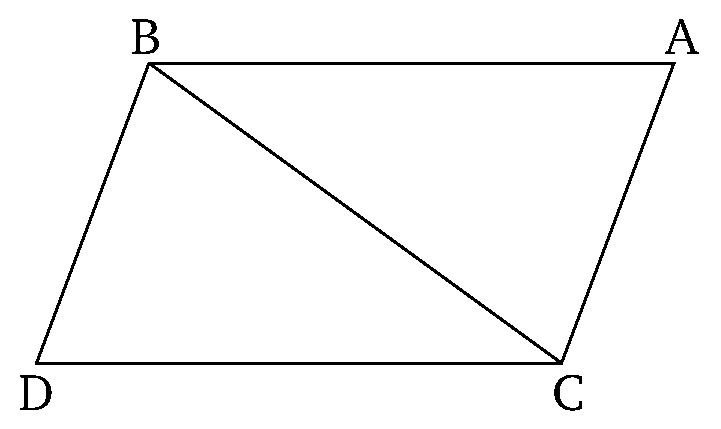
\includegraphics[width=0.5\linewidth]{figures/fig33e.eps}
    \label{fig:prop_33}
    \end{center}
\end{figure*}

Straight-lines joining equal and parallel (straight-lines) on the same sides
are themselves also equal and parallel.

Let $AB$ and $CD$ be equal and parallel (straight-lines), and let the
straight-lines $AC$ and $BD$ join them on the same sides. I say that $AC$
and $BD$ are also equal and parallel.

Let $BC$ have been joined. And since $AB$ is parallel to $CD$, and $BC$ has
fallen across them, the alternate angles $ABC$ and $BCD$ are equal to one another [Prop.~1.29]. And since $AB$ is equal to $CD$, and $BC$ is common,
the two (straight-lines) $AB$, $BC$ are equal to the two (straight-lines)
$DC$, $CB$.$^\dag$And the angle $ABC$ is equal to the angle $BCD$. Thus, the
base $AC$ is equal to the base $BD$, and triangle $ABC$ is equal to triangle
$DCB$$^\ddag$, and the remaining angles will be equal to the corresponding remaining
angles subtended by the equal sides [Prop.~1.4]. Thus,  angle $ACB$ 
is equal to $CBD$. Also, since the straight-line $BC$, (in) falling across the two
straight-lines $AC$ and $BD$, has made the alternate angles  ($ACB$ and $CBD$) equal to one another,
$AC$ is thus parallel to $BD$ [Prop.~1.27]. And ($AC$) was also shown (to be) equal
to ($BD$).

Thus, straight-lines joining equal and parallel (straight-lines) on the same sides
are  themselves also equal and parallel. (Which is) the very thing it was
required to show.


\section*{Commentary}

\begin{proposition}\label{proposition_33}\lean{Elements.Book1.proposition_33}\leanok
    If
\end{proposition}
\begin{proof}
    \uses{proposition_4,proposition_27,proposition_29}\leanok
\end{proof}

\chapter*{Proposition 34}



\begin{figure*}[ht]
    \begin{center}
    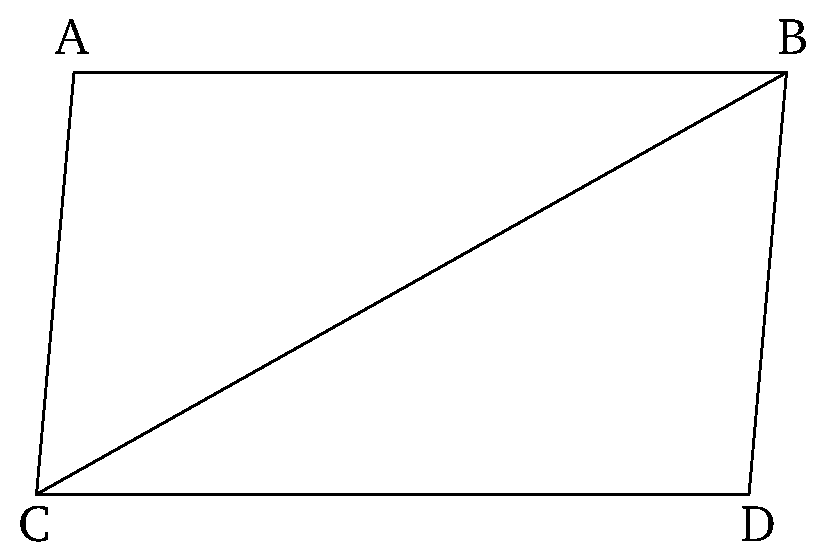
\includegraphics[width=0.5\linewidth]{figures/fig34e.eps}
    \label{fig:prop_34}
    \end{center}
\end{figure*}

In parallelogrammic figures the opposite sides and angles are equal to one
another, and a diagonal cuts them in half.\\

Let $ACDB$ be a parallelogrammic figure, and $BC$ its diagonal. I say that
for parallelogram $ACDB$, the opposite sides and angles are equal to
one another, and the diagonal $BC$ cuts it in half.

For since $AB$ is parallel to $CD$, and the straight-line $BC$ has fallen
across  them, the alternate angles $ABC$ and $BCD$ are equal to one another [Prop.~1.29]. 
Again, since $AC$ is parallel to $BD$, and $BC$ has fallen across them, the
alternate angles $ACB$ and $CBD$ are equal to one another [Prop.~1.29]. 
So $ABC$ and $BCD$ are two triangles having the two angles $ABC$ and
$BCA$ equal to the two (angles) $BCD$ and $CBD$, respectively, and one
side equal to one side---the (one) by the equal angles and common to them, (namely) $BC$. Thus,
they will also  have the remaining sides  equal to the corresponding
remaining (sides), and the remaining angle (equal) to the remaining angle [Prop.~1.26].
Thus, side $AB$ is equal to $CD$, and $AC$ to $BD$. Furthermore, angle $BAC$ is 
equal to $CDB$. And since angle $ABC$ is equal to $BCD$, and $CBD$ to
$ACB$, the whole (angle) $ABD$ is thus equal to the whole (angle) $ACD$.
And  $BAC$ was also shown  (to be) equal to $CDB$.

Thus, in parallelogrammic figures the opposite sides and angles are equal
to one another.

And, I also say that a diagonal cuts them in half. For since $AB$ is equal
to $CD$, and $BC$ (is) common, the two (straight-lines) $AB$, $BC$ are equal
to the two (straight-lines) $DC$, $CB$$^\dag$, respectively. And angle $ABC$ is
equal to angle $BCD$. Thus, the base $AC$ (is) also equal to $DB$, and
triangle $ABC$ is equal to triangle $BCD$ [Prop.~1.4].

Thus, the diagonal $BC$ cuts the parallelogram $ACDB$$^\ddag$ in half. (Which is) the
very thing it was required to show.


\section*{Commentary}

\begin{proposition}\label{proposition_34}\lean{Elements.Book1.proposition_34}\leanok
    If
\end{proposition}
\begin{proof}
    \uses{proposition_26,proposition_29}\leanok
\end{proof}

\chapter*{Proposition 35}



\begin{figure*}[ht]
    \begin{center}
    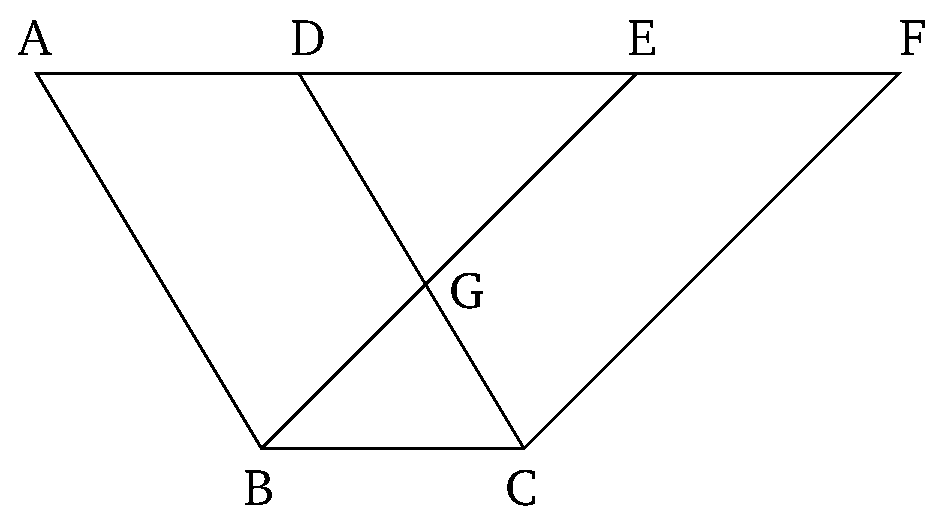
\includegraphics[width=0.5\linewidth]{figures/fig35e.eps}
    \label{fig:prop_35}
    \end{center}
\end{figure*}

Parallelograms which are on the same base and between the same
parallels are equal$^\dag$ to one another.

Let $ABCD$ and $EBCF$ be parallelograms on the same base $BC$, and
between the same parallels $AF$ and $BC$. I say that $ABCD$ is equal to
parallelogram $EBCF$.

For since $ABCD$ is a parallelogram, $AD$ is equal to $BC$ [Prop.~1.34].
So, for the same (reasons), $EF$ is also equal to $BC$. So $AD$ is also equal to
$EF$. And $DE$ is common. Thus, the whole (straight-line) $AE$ is equal
to the whole (straight-line) $DF$.  And $AB$ is also equal to $DC$.
So the two (straight-lines) $EA$, $AB$
are equal to the two (straight-lines) $FD$, $DC$, respectively. And angle $FDC$ is
equal to angle $EAB$, the external to the internal [Prop.~1.29]. Thus, the
base $EB$ is equal to the base $FC$, and triangle $EAB$ will be equal to triangle
$DFC$ [Prop.~1.4]. Let $DGE$ have been taken away from both. 
Thus, the remaining trapezium $ABGD$ is equal to the remaining trapezium
$EGCF$. Let triangle $GBC$ have been added to both. Thus, the whole
parallelogram $ABCD$ is equal to the whole parallelogram $EBCF$.

Thus, parallelograms which are on the same base and between the same
parallels are equal to one another. (Which is) the very thing it was required to
show.



\section*{Commentary}

\begin{proposition}\label{proposition_35}\lean{Elements.Book1.proposition_35}\leanok
    If
\end{proposition}
\begin{proof}
    \uses{proposition_4,proposition_29,proposition_34}\leanok
\end{proof}

\chapter*{Proposition 36}



\begin{figure*}[ht]
    \begin{center}
    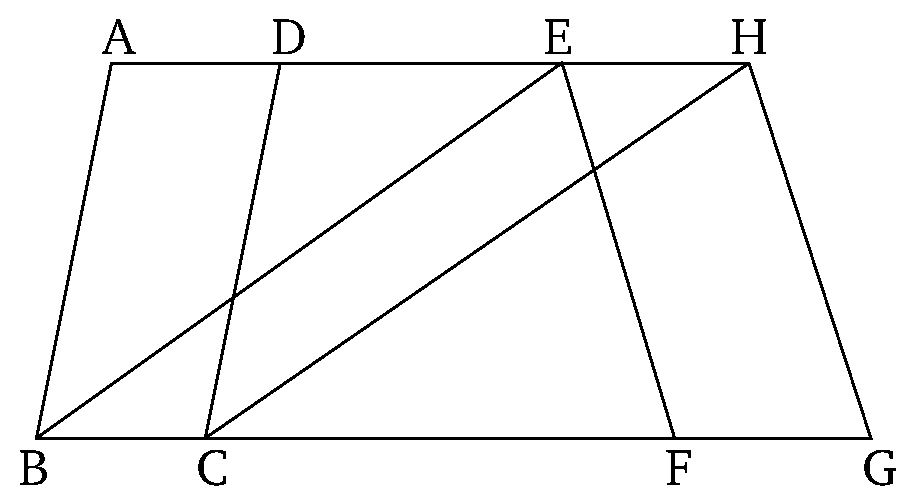
\includegraphics[width=0.5\linewidth]{figures/fig36e.eps}
    \label{fig:prop_36}
    \end{center}
\end{figure*}

Parallelograms which are on equal bases and between the same parallels are equal to one another.

Let $ABCD$ and $EFGH$ be parallelograms which are on the equal bases $BC$
and $FG$, and (are) between the same parallels $AH$ and $BG$. I say that
the parallelogram $ABCD$ is equal to $EFGH$.

For let $BE$ and $CH$ have been joined. And since $BC$ is equal to $FG$, but $FG$ is equal to $EH$ [Prop.~1.34], $BC$ is thus equal to $EH$. And they are also parallel, and $EB$ and $HC$ join them.
But (straight-lines) joining equal and parallel (straight-lines) on the
same sides are (themselves) equal and parallel [Prop.~1.33] [thus, $EB$ and $HC$
are also equal and parallel]. Thus, $EBCH$ is a parallelogram [Prop.~1.34],
and is equal to $ABCD$. For it has  the
same base, $BC$, as ($ABCD$), and is between the same parallels, $BC$ and $AH$, as ($ABCD$) [Prop.~1.35]. So,
for the same (reasons), $EFGH$ is also equal to the same (parallelogram) $EBCH$ [Prop.~1.34].  So that the
parallelogram $ABCD$ is  also equal to $EFGH$.

Thus, parallelograms which are on equal bases and between the same parallels are equal to one another. (Which is) the very thing it was required
to show.


\section*{Commentary}

\begin{proposition}\label{proposition_36}\lean{Elements.Book1.proposition_36}\leanok
    If
\end{proposition}
\begin{proof}
    \uses{proposition_33,proposition_34,proposition_35}\leanok
\end{proof}

\chapter*{Proposition 37}



\begin{figure*}[ht]
    \begin{center}
    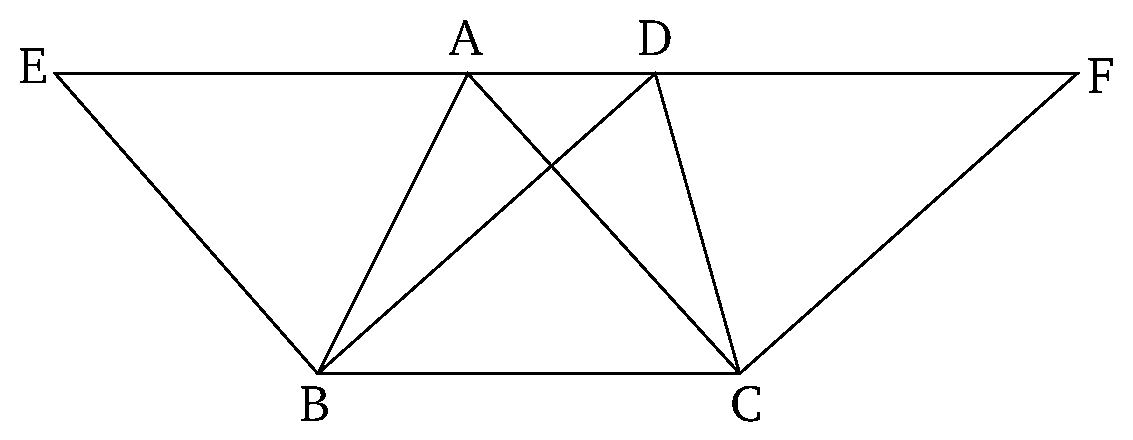
\includegraphics[width=0.5\linewidth]{figures/fig37e.eps}
    \label{fig:prop_37}
    \end{center}
\end{figure*}

Triangles which are on the same base and between the same parallels
are equal to one another.

Let $ABC$ and $DBC$ be triangles on the same base $BC$, and between
the same parallels $AD$ and $BC$. I say that triangle $ABC$ is equal to triangle $DBC$.

Let $AD$ have been produced in both directions to $E$ and $F$, and let the
(straight-line) $BE$ have been drawn through $B$ parallel to $CA$ [Prop.~1.31],
and let the (straight-line) $CF$ have been drawn through $C$ parallel to
$BD$ [Prop.~1.31]. Thus, $EBCA$ and $DBCF$ are both parallelograms,
and are equal. For they are on the same base $BC$, and between
the same parallels $BC$ and $EF$ [Prop.~1.35]. And the triangle $ABC$ is
half of 
the parallelogram
$EBCA$. For the diagonal $AB$ cuts the latter in half [Prop.~1.34]. And the 
triangle $DBC$ (is) half of the parallelogram $DBCF$. For the diagonal
$DC$ cuts the latter in half [Prop.~1.34]. [And the halves of equal things are
equal to one another.]$^\dag$
Thus, triangle $ABC$ is equal to triangle $DBC$.

Thus, triangles which are on the same base and between the same parallels
are equal to one another. (Which is) the very thing it was required to show.


\section*{Commentary}

\begin{proposition}\label{proposition_37}\lean{Elements.Book1.proposition_37}\leanok
    If
\end{proposition}
\begin{proof}
    \uses{proposition_31,proposition_33,proposition_35}\leanok
\end{proof}

\chapter*{Proposition 38}



\begin{figure*}[ht]
    \begin{center}
    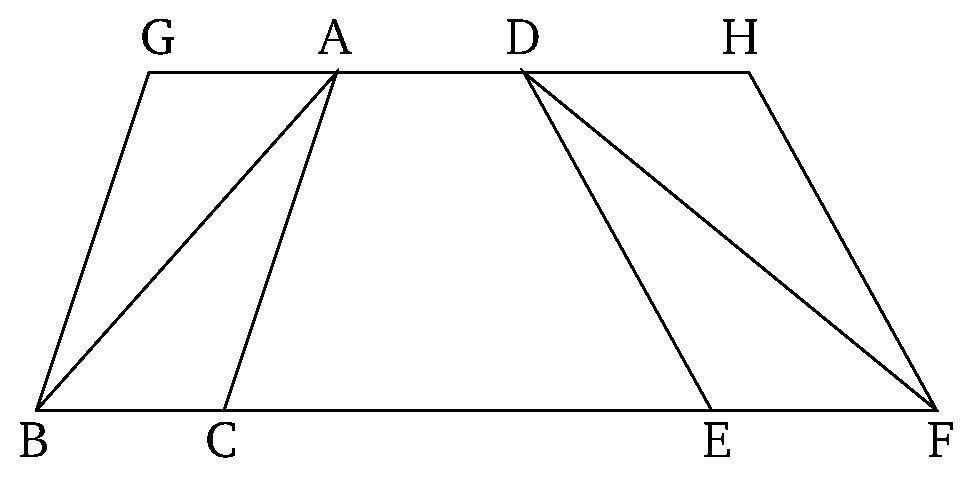
\includegraphics[width=0.5\linewidth]{figures/fig38e.eps}
    \label{fig:prop_38}
    \end{center}
\end{figure*}

Triangles which are on equal bases and between the same parallels
are equal to one another.

Let $ABC$ and $DEF$ be triangles on the equal bases $BC$ and $EF$, and between the same parallels $BF$ and $AD$. I say that triangle $ABC$ is equal to triangle $DEF$.

For let $AD$ have been produced in both directions to $G$ and $H$, and
let the (straight-line) $BG$ have been drawn through $B$ parallel to $CA$ [Prop.~1.31], and let the (straight-line) $FH$ have been drawn through
$F$ parallel to $DE$ [Prop.~1.31]. Thus,  $GBCA$ and $DEFH$ are
each parallelograms. And $GBCA$ is equal to $DEFH$.
For they are on the equal bases $BC$ and $EF$, and between  the same
parallels $BF$ and $GH$ [Prop.~1.36]. And triangle $ABC$ is half of the parallelogram
$GBCA$. For the diagonal $AB$ cuts the latter in half [Prop.~1.34]. And
triangle $FED$ (is) half of parallelogram $DEFH$. For the diagonal $DF$ cuts
the latter in half. [And the halves of equal things are equal to one another.] Thus,
triangle $ABC$ is equal to triangle $DEF$.

Thus, triangles which are on equal bases and between the same parallels
are equal to one another. (Which is) the very thing it was required to show.



\section*{Commentary}

\begin{proposition}\label{proposition_38}\lean{Elements.Book1.proposition_38}\leanok
    If
\end{proposition}
\begin{proof}
    \uses{proposition_31,proposition_34,proposition_36}\leanok
\end{proof}

\chapter*{Proposition 39}



\begin{figure*}[ht]
    \begin{center}
    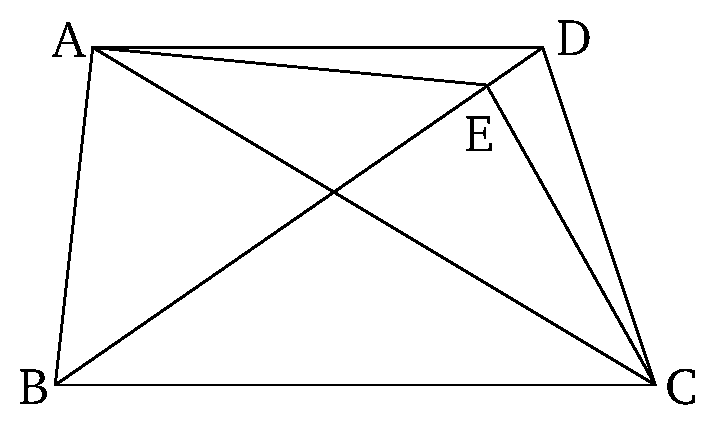
\includegraphics[width=0.5\linewidth]{figures/fig39e.eps}
    \label{fig:prop_39}
    \end{center}
\end{figure*}

Equal triangles which are on the same base, and on the same side, are
also between the same parallels.

Let $ABC$ and $DBC$ be equal triangles which are on the same base $BC$,
and on the same side (of it). I say that they are also between the same parallels.

For let $AD$ have been joined. I say that $AD$ and $BC$ are parallel.

For, if not, let $AE$ have been drawn through point A parallel to the straight-line $BC$ [Prop.~1.31], and let $EC$ have been joined. Thus, triangle $ABC$ is equal
to triangle $EBC$. For it is on the same base as it, $BC$, and between the
same parallels [Prop.~1.37]. But $ABC$ is equal to $DBC$. Thus, $DBC$ is
also equal to $EBC$, the greater to the lesser. The very thing is impossible.
Thus, $AE$ is not parallel to $BC$. Similarly, we can show that neither (is)
any other (straight-line) than $AD$. Thus, $AD$ is parallel to $BC$.

Thus, equal triangles which are on the same base, and on the same side, are
also between the same parallels. (Which is) the very thing it was required to show.


\section*{Commentary}

\begin{proposition}\label{proposition_39}\lean{Elements.Book1.proposition_39}\leanok
    If
\end{proposition}
\begin{proof}
    \uses{proposition_31,proposition_37}\leanok
\end{proof}

\chapter*{Proposition 40}



\begin{figure*}[ht]
    \begin{center}
    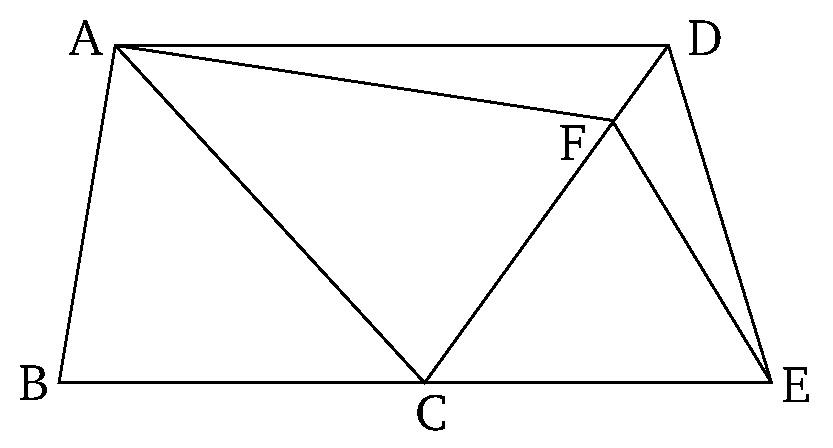
\includegraphics[width=0.5\linewidth]{figures/fig40e.eps}
    \label{fig:prop_40}
    \end{center}
\end{figure*}

Equal triangles which are on equal bases, and on the same side, are also
between the same parallels.

Let $ABC$ and $CDE$ be equal triangles on the equal bases $BC$ and $CE$ (respectively), and on the same side (of $BE$). I say that they are also between
the same parallels.

For let $AD$ have been joined. I say that $AD$ is parallel to $BE$.

For if not, let $AF$ have been drawn through $A$ parallel to $BE$ [Prop.~1.31],
and let $FE$ have been joined. Thus, triangle $ABC$ is equal to triangle
$FCE$. For they are on equal bases, $BC$ and $CE$, and between the same
parallels, $BE$ and $AF$ [Prop.~1.38]. But, triangle $ABC$ is equal to [triangle] $DCE$.
Thus, [triangle] $DCE$ is also equal to triangle $FCE$, the greater to the
lesser. The very thing is impossible. 
Thus, $AF$ is not parallel to $BE$. Similarly, we can show that neither (is)
any other (straight-line) than $AD$. Thus, $AD$ is parallel to $BE$.

Thus, equal triangles which are on equal bases, and on the same side, are also
between the same parallels. (Which is) the very thing it was required to show.


\section*{Commentary}

\begin{proposition}\label{proposition_40}\lean{Elements.Book1.proposition_40}\leanok
    If
\end{proposition}
\begin{proof}
    \uses{proposition_31,proposition_38}\leanok
\end{proof}

\chapter*{Proposition 41}



\begin{figure*}[ht]
    \begin{center}
    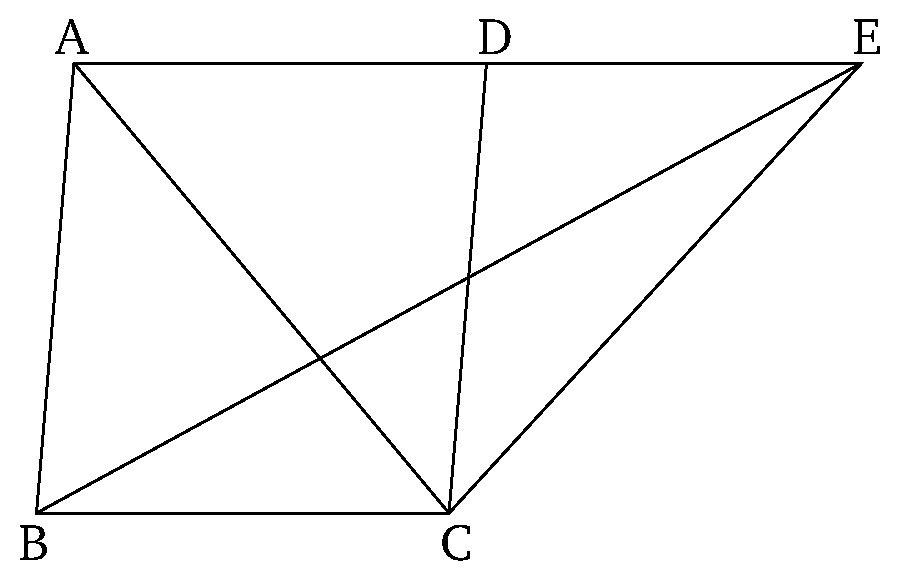
\includegraphics[width=0.5\linewidth]{figures/fig41e.eps}
    \label{fig:prop_41}
    \end{center}
\end{figure*}

If a parallelogram has the same base as a triangle, and is between
the same parallels, then the parallelogram is double (the area) of the triangle.

For let parallelogram $ABCD$ have the same base $BC$ as triangle $EBC$,
and let it be between the same parallels, $BC$ and $AE$. I say that 
parallelogram $ABCD$ is double (the area) of triangle $BEC$.

For let $AC$ have been joined. So triangle $ABC$ is equal to triangle
$EBC$. For it is on the same base, $BC$,  as ($EBC$), and between the same
parallels, $BC$ and $AE$ [Prop.~1.37]. But, parallelogram $ABCD$
is double (the area) of triangle $ABC$. For the diagonal $AC$ cuts
the former in half [Prop.~1.34]. So parallelogram $ABCD$ is also
double (the area) of triangle $EBC$.

Thus, if a parallelogram has the same base as a triangle, and is between
the same parallels, then the parallelogram is double (the area) of the triangle.
(Which is) the very thing it was required to show.


\section*{Commentary}

\begin{proposition}\label{proposition_41}\lean{Elements.Book1.proposition_41}\leanok
    If
\end{proposition}
\begin{proof}
    \uses{proposition_34,proposition_37}\leanok
\end{proof}

\chapter*{Proposition 42}



\begin{figure*}[ht]
    \begin{center}
    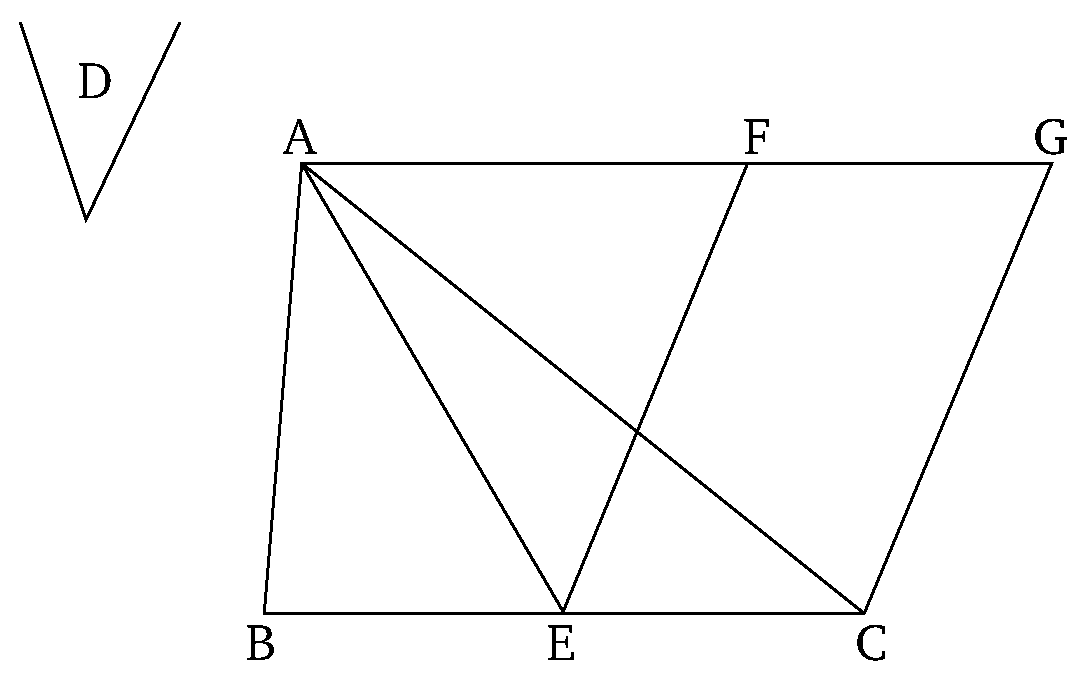
\includegraphics[width=0.5\linewidth]{figures/fig42e.eps}
    \label{fig:prop_42}
    \end{center}
\end{figure*}

To construct a parallelogram equal to a given triangle in a given
rectilinear angle.

Let $ABC$ be the given triangle, and $D$ the given rectilinear angle. So
it is required to construct a parallelogram equal to triangle $ABC$
in the rectilinear angle $D$.

Let $BC$ have been cut in half at $E$ [Prop.~1.10], and let $AE$ have been joined. And let (angle) $CEF$, equal to angle $D$,  have been constructed
at the point $E$ on the straight-line $EC$ [Prop.~1.23]. And let $AG$ have been drawn through $A$
parallel to $EC$ [Prop.~1.31], and let $CG$ have been drawn through $C$ parallel
to $EF$ [Prop.~1.31]. Thus, $FECG$ is a parallelogram. And since $BE$ is
equal to $EC$, triangle $ABE$ is also equal to triangle $AEC$. For they are
on the equal bases, $BE$ and $EC$, and between the same parallels, $BC$ and $AG$ [Prop.~1.38]. Thus, triangle $ABC$ is double (the area) of triangle $AEC$. And
parallelogram $FECG$ is also double (the area) of triangle $AEC$. For it has the same base as ($AEC$), and is between the same parallels  as ($AEC$) [Prop.~1.41].
Thus, parallelogram $FECG$ is equal to triangle $ABC$.  ($FECG$) also has
the angle $CEF$ equal to the given (angle) $D$.

Thus, parallelogram $FECG$,  equal to the given
triangle $ABC$, has been constructed in the angle $CEF$, which is equal to $D$. (Which is) the
very thing it was required to do.


\section*{Commentary}

\begin{proposition}\label{proposition_42}\lean{Elements.Book1.proposition_42}\leanok
    If
\end{proposition}
\begin{proof}
    \uses{proposition_10,proposition_23,proposition_31,proposition_38,proposition_41}\leanok
\end{proof}

\chapter*{Proposition 43}



\begin{figure*}[ht]
    \begin{center}
    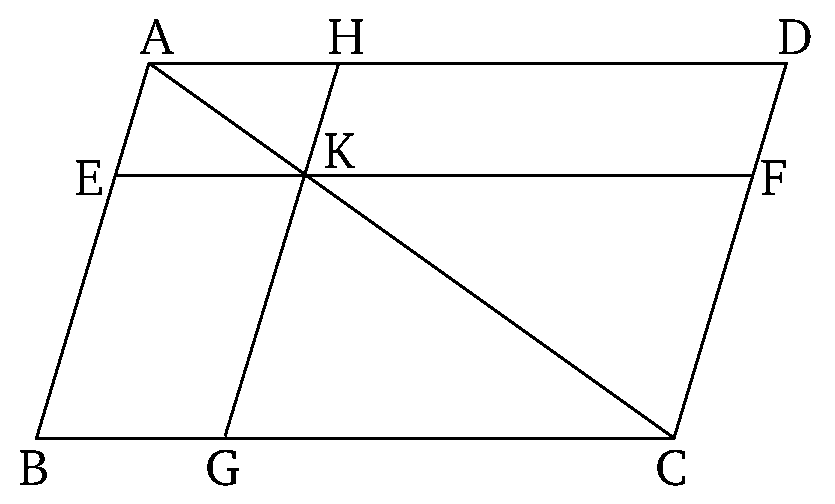
\includegraphics[width=0.5\linewidth]{figures/fig43e.eps}
    \label{fig:prop_43}
    \end{center}
\end{figure*}

For any parallelogram, the complements of the parallelograms about the diagonal are equal to one another.

Let $ABCD$ be a parallelogram, and $AC$ its diagonal. And let $EH$ and $FG$
be the parallelograms about  $AC$, and $BK$ and $KD$ the so-called complements
(about $AC$).
I say that the complement $BK$ is equal to the complement $KD$.

For since $ABCD$ is a parallelogram, and $AC$ its diagonal,  triangle
$ABC$ is equal to triangle $ACD$ [Prop.~1.34]. Again, since $EH$ is
a parallelogram, and $AK$ is its diagonal, triangle $AEK$ is equal to
triangle $AHK$ [Prop.~1.34]. So, for the same (reasons), triangle
$KFC$ is also equal to (triangle) $KGC$. Therefore, since triangle $AEK$ is
equal to triangle $AHK$, and $KFC$ to $KGC$, triangle $AEK$ plus $KGC$ is
equal to triangle $AHK$ plus $KFC$. And the whole triangle $ABC$ is
also equal to the whole (triangle) $ADC$. Thus, the remaining complement
$BK$ is equal to the remaining complement $KD$.

Thus, for any parallelogramic figure, the complements of the
parallelograms about the diagonal are equal to one another.
(Which is) the very thing it was required to show.


\section*{Commentary}

\begin{proposition}\label{proposition_43}\lean{Elements.Book1.proposition_43}\leanok
    If
\end{proposition}
\begin{proof}
    \uses{proposition_34}\leanok
\end{proof}

\chapter*{Proposition 44}



\begin{figure*}[ht]
    \begin{center}
    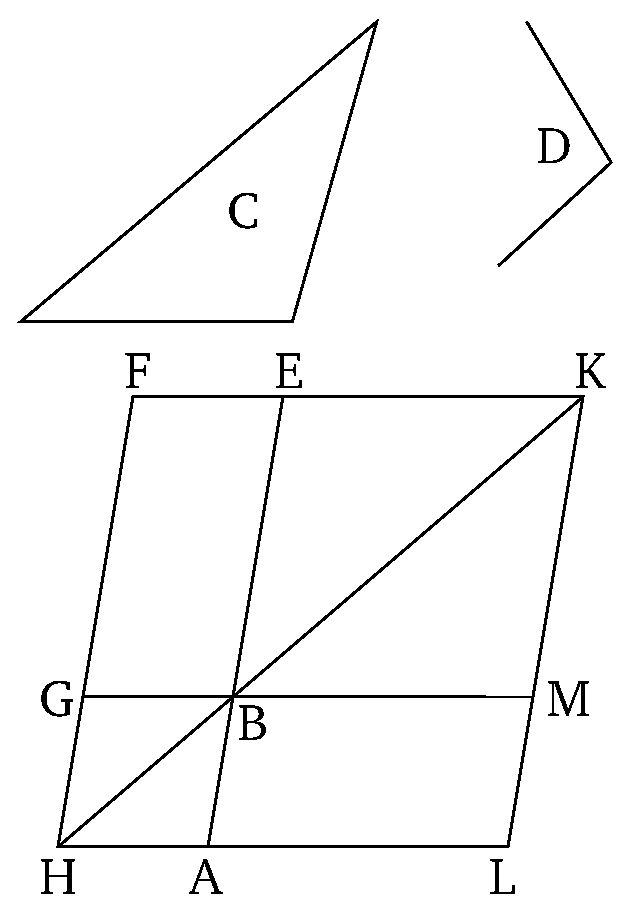
\includegraphics[width=0.5\linewidth]{figures/fig44e.eps}
    \label{fig:prop_44}
    \end{center}
\end{figure*}

To apply a parallelogram equal to a given triangle to a given straight-line
in a given rectilinear angle.\\

Let $AB$ be the given straight-line,  $C$ the given triangle, and $D$ the
given rectilinear angle. So it is required to apply a parallelogram
equal to the given triangle $C$ to the given straight-line $AB$ in an angle equal to (angle) $D$.

Let the parallelogram $BEFG$, equal to the triangle $C$, have been
constructed in the angle $EBG$, which is equal to $D$ [Prop.~1.42].
And let it have been placed so that $BE$ is straight-on to $AB$.$^\dag$  And
let $FG$ have been drawn through to $H$, and let $AH$ have been
drawn through A parallel to either of $BG$ or $EF$ [Prop.~1.31], and
let $HB$ have been joined. And since the straight-line $HF$ falls across the
parallels $AH$ and $EF$, the (sum of the) angles $AHF$ and $HFE$ is thus equal to
two right-angles [Prop.~1.29]. Thus, (the sum of) $BHG$ and $GFE$ is less than two
right-angles.
And (straight-lines) produced to
infinity from (internal angles whose sum is) less than two right-angles meet together [Post.~\ref{post:5}].
Thus, being produced, $HB$ and $FE$ will meet together. Let them have
been produced, and let them meet together at $K$. And let $KL$ have been
drawn through point $K$ parallel to either of $EA$ or $FH$ [Prop.~1.31]. And
let $HA$ and $GB$ have been produced to points $L$ and $M$ (respectively). Thus, $HLKF$ is a parallelogram, and $HK$ its diagonal. And $AG$ and $ME$ (are) parallelograms, and $LB$ and $BF$ the so-called complements, about $HK$. Thus, $LB$ is
equal to $BF$ [Prop.~1.43]. But, $BF$ is equal to triangle $C$. Thus, $LB$ is also
equal to $C$. Also, since angle $GBE$ is equal to $ABM$ [Prop.~1.15], but
$GBE$ is equal to $D$, $ABM$ is thus also equal to angle $D$.

Thus, the parallelogram $LB$, equal to the
given triangle $C$, has been applied to the given straight-line
$AB$ in the angle $ABM$, which is equal to $D$. (Which is) the very thing it was required to do.


\section*{Commentary}

\begin{proposition}\label{proposition_44}\lean{Elements.Book1.proposition_44}\leanok
    If
\end{proposition}
\begin{proof}
    \uses{proposition_15,proposition_29,proposition_30,proposition_31,proposition_42,proposition_43}\leanok
\end{proof}

\chapter*{Proposition 45}



\begin{figure*}[ht]
    \begin{center}
    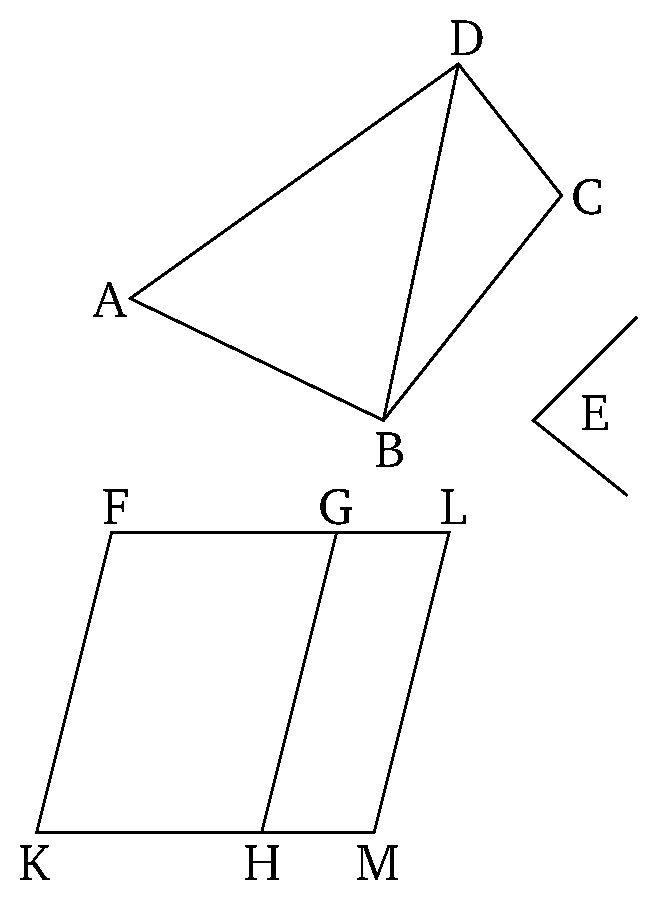
\includegraphics[width=0.5\linewidth]{figures/fig45e.eps}
    \label{fig:prop_45}
    \end{center}
\end{figure*}

To construct a parallelogram equal to a given rectilinear figure in a given
rectilinear angle.

Let $ABCD$ be the given rectilinear figure,$^\dag$ and $E$ the given rectilinear angle.
So it is required to construct a parallelogram equal to the rectilinear figure
$ABCD$ in the given angle $E$.

Let $DB$ have been joined, and let the parallelogram $FH$, equal to
the triangle $ABD$, have been
constructed in the angle $HKF$, which is equal to $E$ [Prop.~1.42].
And let the parallelogram $GM$, equal to the triangle $DBC$, have been
applied to the straight-line $GH$ in the angle $GHM$,
which is equal to $E$ [Prop.~1.44]. And since angle $E$ is equal to each of
(angles) $HKF$ and $GHM$,  (angle) $HKF$ is thus also equal to $GHM$. 
Let $KHG$ have been added to both. Thus, (the sum of) $FKH$ and $KHG$ is
equal to (the sum of) $KHG$ and $GHM$. But, (the sum of) $FKH$ and $KHG$ is equal to
two right-angles [Prop.~1.29]. Thus, (the sum of) $KHG$ and $GHM$ is also equal to
two right-angles. So two straight-lines, $KH$ and $HM$, not lying on the same side, make  adjacent angles with some straight-line $GH$, 
at the point $H$ on it, (whose sum is) equal to two right-angles.
Thus, $KH$ is straight-on to $HM$ [Prop.~1.14].
And since the straight-line $HG$ falls across the parallels $KM$ and $FG$, the alternate angles
$MHG$ and $HGF$ are equal to one another [Prop.~1.29]. Let $HGL$ have
been added to both. Thus, (the sum of) $MHG$ and $HGL$ is equal to 
(the sum of) $HGF$ and $HGL$.
But, (the sum of) $MHG$ and $HGL$ is equal to two right-angles [Prop.~1.29].
Thus, (the sum of) $HGF$ and $HGL$ is also equal to two right-angles.
Thus, $FG$ is straight-on to $GL$ [Prop.~1.14]. And since $FK$ is
equal and parallel to $HG$ [Prop.~1.34], but also $HG$ to $ML$ [Prop.~1.34],
$KF$ is thus also equal and parallel to $ML$ [Prop.~1.30]. And the straight-lines $KM$ and
$FL$ join them. Thus, $KM$ and $FL$ are equal and parallel as well [Prop.~1.33].
Thus, $KFLM$ is a parallelogram. And since triangle $ABD$ is equal to parallelogram $FH$, and $DBC$ to $GM$, the whole rectilinear figure
$ABCD$ is thus equal to the whole parallelogram $KFLM$.

Thus, the parallelogram $KFLM$, equal to the given
rectilinear figure $ABCD$, has been constructed in the angle
$FKM$, which is equal to the given (angle) $E$. (Which is) the very thing it was
required to do.


\section*{Commentary}

\begin{proposition}\label{proposition_45}\lean{Elements.Book1.proposition_45}\leanok
    If
\end{proposition}
\begin{proof}
    \uses{proposition_14,proposition_29,proposition_30,proposition_33,proposition_34,proposition_42,proposition_44}\leanok
\end{proof}

\chapter*{Proposition 46}



\begin{figure*}[ht]
    \begin{center}
    \includegraphics[width=0.5\linewidth]{figures/fig46e.eps}
    \label{fig:prop_46}
    \end{center}
\end{figure*}

To describe a square on a given straight-line.

Let $AB$ be the given straight-line. So it is required to describe a
square on the straight-line $AB$.

Let $AC$ have been drawn at right-angles to the straight-line $AB$
from the point $A$ on it [Prop.~1.11], and let $AD$ have been
made equal to $AB$ [Prop.~1.3]. And let $DE$ have been drawn
through point $D$ parallel to $AB$ [Prop.~1.31], and let $BE$ have been
drawn through point $B$ parallel to $AD$ [Prop.~1.31]. Thus,
$ADEB$ is a parallelogram. Therefore, $AB$ is equal to $DE$, and $AD$ to $BE$ [Prop.~1.34]. But, $AB$ is equal to $AD$. Thus, the four (sides) $BA$, $AD$, $DE$, and $EB$ are equal to one another. Thus, the parallelogram $ADEB$ is equilateral.
So I say that (it is) also right-angled. For since the straight-line $AD$ falls
across the parallels $AB$ and $DE$, the (sum of the) angles $BAD$ and $ADE$ is
equal to two right-angles [Prop.~1.29]. But $BAD$ (is a) right-angle. Thus,
$ADE$ (is) also a right-angle. And for parallelogrammic figures, the opposite
sides and angles are equal to one another [Prop.~1.34]. Thus, each of the
opposite angles $ABE$ and $BED$ (are) also right-angles. Thus, $ADEB$ is
right-angled. And it was also shown (to be) equilateral.

Thus, ($ADEB$) is a square [Def.~\ref{def:22}]. And it is described on the straight-line $AB$. (Which is) the very thing it was required to do.


\section*{Commentary}

\begin{proposition}\label{proposition_46}\lean{Elements.Book1.proposition_46}\leanok
    If
\end{proposition}
\begin{proof}
    \uses{proposition_3,proposition_11,proposition_29,proposition_31,proposition_34}\leanok
\end{proof}

\chapter*{Proposition 47}



\begin{figure*}[ht]
    \begin{center}
    \includegraphics[width=0.5\linewidth]{figures/fig47e.eps}
    \label{fig:prop_47}
    \end{center}
\end{figure*}

In right-angled triangles,  the square on the side subtending the right-angle
is equal to the (sum of the) squares on the sides containing the right-angle.

Let $ABC$ be a right-angled triangle having the angle $BAC$a right-angle. I say that the
square on $BC$ is equal to the (sum of the) squares on $BA$ and $AC$.

For let the square $BDEC$ have been described on $BC$, and (the squares) $GB$ and $HC$ on $AB$ and $AC$ (respectively) [Prop.~1.46]. And let $AL$ have been drawn through point $A$ parallel to either of $BD$ or $CE$ [Prop.~1.31]. And let $AD$ and $FC$ have been joined. And
since angles $BAC$ and $BAG$ are each right-angles, then two straight-lines $AC$ and $AG$, not lying on the same side,
make the adjacent angles with some straight-line $BA$, at the point
$A$ on it, (whose sum is) equal to two right-angles. Thus, $CA$ is straight-on to $AG$ [Prop.~1.14]. So, for
the same (reasons), $BA$ is also straight-on to $AH$. And since angle $DBC$ is
equal to $FBA$, for (they are) both right-angles, let $ABC$ have been added to
both.  Thus, the whole (angle) $DBA$ is equal to the whole (angle) $FBC$.
And since $DB$ is equal to $BC$, and $FB$ to $BA$, the two (straight-lines) $DB$,
$BA$ are equal to the two (straight-lines) $CB$, $BF$,$^\dag$ respectively. And angle $DBA$ (is) equal to angle $FBC$. Thus, the base $AD$ [is] equal to the base $FC$,
and the triangle $ABD$ is equal to the triangle $FBC$ [Prop.~1.4]. And 
parallelogram $BL$ [is] double (the area) of triangle $ABD$. For they
have the same base, $BD$, and are between the same parallels, $BD$ and $AL$  [Prop.~1.41]. And
 square
$GB$ is double (the area) of triangle $FBC$. For again they have the same base, $FB$, and
are between the same parallels,
$FB$ and $GC$ [Prop.~1.41]. [And the doubles of equal things
are equal to one another.]$^\ddag$ Thus, the parallelogram $BL$ is also equal to the square $GB$. So, similarly, $AE$ and $BK$ being joined, 
the parallelogram $CL$ can be shown (to be)  equal to the square $HC$. Thus, the whole square
$BDEC$ is equal to the (sum of the) two squares $GB$ and $HC$. And the square $BDEC$
is described on $BC$, and the (squares) $GB$ and $HC$ on $BA$ and $AC$ (respectively). Thus, the square on the side $BC$ is equal to the
(sum of the) squares
on the sides $BA$ and $AC$.

Thus, in right-angled triangles,  the square on the side subtending the right-angle
is equal to the (sum of the) squares on the sides surrounding the right-[angle].
(Which is) the very thing it was required to show.


\section*{Commentary}

\begin{proposition}\label{proposition_47}\lean{Elements.Book1.proposition_47}\leanok
    If
\end{proposition}
\begin{proof}
    \uses{proposition_4,proposition_13,proposition_14,proposition_16,proposition_17,proposition_30,proposition_31,proposition_41,proposition_46}\leanok
\end{proof}

\chapter*{Proposition 48}



\begin{figure*}[ht]
    \begin{center}
    \includegraphics[width=0.5\linewidth]{figures/fig48e.eps}
    \label{fig:prop_48}
    \end{center}
\end{figure*}


If the square on one of the sides of a triangle is equal to the (sum of the)
squares on the two remaining sides of the triangle then the angle contained
by the two remaining sides of the triangle is a right-angle.

For let the square on one of the sides, $BC$, of triangle $ABC$ be equal
to the (sum of the) squares on the sides $BA$ and $AC$. I say that angle
$BAC$ is a right-angle.

For let $AD$ have been drawn from point $A$ at right-angles to the
straight-line $AC$ [Prop.~1.11], and let $AD$ have been made equal to
$BA$ [Prop.~1.3], and let $DC$ have been joined. Since $DA$ is equal to $AB$,
the square on $DA$ is thus also equal to the square on $AB$.$^\dag$ Let the square on
$AC$ have been added to both. Thus, the (sum of the) squares on $DA$ and $AC$ is equal
to the (sum of the) squares on $BA$ and $AC$. But, the (square) on $DC$ 
is equal to the (sum of the squares) on $DA$ and $AC$. For angle $DAC$ is a right-angle [Prop.~1.47].
But, the  (square) on $BC$ is equal to (sum of the squares) on $BA$ and $AC$.
For (that) was assumed. Thus, the square on $DC$ is equal to the square on $BC$.
So  side $DC$ is also equal to (side) $BC$. And since $DA$ is equal to $AB$, and $AC$ (is) common, the two (straight-lines) $DA$, $AC$ are equal to the two (straight-lines)
$BA$, $AC$. And the base $DC$ is equal to the base $BC$. Thus, angle $DAC$ [is] equal to angle $BAC$ [Prop.~1.8].  But $DAC$ is a right-angle. Thus, $BAC$ is
also a right-angle.

Thus, if the square on one of the sides of a triangle is equal to the (sum of the)
squares on the remaining two sides of the triangle then the angle contained
by the remaining two sides of the triangle is a right-angle. (Which is) the very thing
it was required to show.


\section*{Commentary}

\begin{proposition}\label{proposition_48}\lean{Elements.Book1.proposition_48}\leanok
    If
\end{proposition}
\begin{proof}
    \uses{proposition_3,proposition_8,proposition_11,proposition_47}\leanok
\end{proof}


\end{document}


\github{https://github.com/loganrjmurphy/lean-geo-lib/}
\dochome{https://loganrjmurphy.github.io/lean-geo-lib/docs}

\title{The First Book of Euclid's Elements---Commentary and Lean Formalization}
\author{
    Logan Murphy$^{1}$, Jack Sun$^{1}$, Zhaoyu Li$^{1}$, Anima Anandkumar$^{2}$, Xujie Si$^{1\,\dagger}$, and Kaiyu Yang$^{2\,\dagger}$\\
    $^1$University of Toronto, ~$^2$Caltech\\
    $^\dagger$ Equal advising \\
}

\begin{document}
\maketitle
\chapter{Introduction}

\chapter{Definitions}

\begin{enumerate}
    \item \label{def:1} A point is that of which there is no part.
    \item \label{def:2} And a line is a length without breadth.
    \item \label{def:3} And the extremities of a line are points.
    \item \label{def:4} A straight-line is (any) one which lies evenly with points on itself.
    \item \label{def:5} And a surface is that which has length and breadth only.
    \item \label{def:6} And the extremities of a surface are lines.
    \item \label{def:7} A plane surface is (any) one which lies evenly with the straight-lines on itself.
    \item \label{def:8} And a plane angle is the inclination of the lines to one another, when two lines in a plane meet one another, and are not lying in a straight-line.
    \item \label{def:9} And when the lines containing the angle are straight then the angle is called rectilinear.
    \item \label{def:10} And when a straight-line stood upon (another) straight-line makes adjacent angles (which are) equal to one another, each of the equal angles is a right-angle, and the former straight-line is called a perpendicular to that upon which it stands.
    \item \label{def:11} An obtuse angle is one greater than a right-angle.
    \item \label{def:12} And an acute angle (is) one less than a right-angle.
    \item \label{def:13} A boundary is that which is the extremity of something.
    \item \label{def:14} A figure is that which is contained by some boundary or boundaries.
    \item \label{def:15} A circle is a plane figure contained by a single line [which is called a circumference], (such that) all of the straight-lines radiating towards [the circumference] from one point amongst those lying inside the figure are equal to one another.
    \item \label{def:16} And the point is called the center of the circle.
    \item \label{def:17} And a diameter of the circle is any straight-line, being drawn through the center, and terminated in each direction by the circumference of the circle. (And) any such (straight-line) also cuts the circle in half.
    \item \label{def:18} And a semi-circle is the figure contained by the diameter and the circumference cuts off by it. And the center of the semi-circle is the same (point) as (the center of) the circle.
    \item \label{def:19} Rectilinear figures are those (figures) contained by straight-lines: trilateral figures being those contained by three straight-lines, quadrilateral by four, and multilateral by more than four.
    \item \label{def:20} And of the trilateral figures: an equilateral triangle is that having three equal sides, an isosceles (triangle) that having only two equal sides, and a scalene (triangle) that having three unequal sides.
    \item \label{def:21} And further of the trilateral figures: a right-angled triangle is that having a right-angle, an obtuse-angled (triangle) that having an obtuse angle, and an acute-angled (triangle) that having three acute angles.
    \item \label{def:22} And of the quadrilateral figures: a square is that which is right-angled and equilateral, a rectangle that which is right-angled but not equilateral, a rhombus that which is equilateral but not right-angled, and a rhomboid that having opposite sides and angles equal to one another which is neither right-angled nor equilateral. And let quadrilateral figures besides these be called trapezia.
    \item \label{def:23} Parallel lines are straight-lines which, being in the same plane, and being produced to infinity in each direction, meet with one another in neither (of these directions).
\end{enumerate}
\chapter{Postulates}

\begin{enumerate}
    \item \label{post:1} Let it have been postulated to draw a straight-line from any point to any point.
    \item \label{post:2} And to produce a finite straight-line continuously in a straight-line.
    \item \label{post:3} And to draw a circle with any center and radius.
    \item \label{post:4} And that all right-angles are equal to one another.
    \item \label{post:5} And that if a straight-line falling across two (other) straight-lines makes internal angles on the same side (of itself whose sum is) less than two right-angles, then the two (other) straight-lines, being produced to infinity, meet on that side (of the original straight-line) that the (sum of the internal angles) is less than two right-angles (and do not meet on the other side).
\end{enumerate}

\chapter{Common Notions}

\begin{enumerate}
    \item \label{cn:1} Things equal to the same thing are also equal to one another.
    \item \label{cn:2} And if equal things are added to equal things then the wholes are equal.
    \item \label{cn:3} And if equal things are subtracted from equal things then the remainders are equal.
    \item \label{cn:4} And things coinciding with one another are equal to one another.
    \item \label{cn:5} And the whole [is] greater than the part.
\end{enumerate}



\chapter*{Proposition 1}
\label{prop:1}

\begin{figure*}[ht]
    \begin{center}
    \includegraphics[width=0.5\linewidth]{figures/fig01e.eps}
    \label{fig:prop_1}
    \end{center}
\end{figure*}

To construct an equilateral triangle on a given finite straight-line.

Let $AB$ be the given finite straight-line. 

So it is required to construct an equilateral triangle on the straight-line $AB$.

Let the circle $BCD$ with center $A$ and radius $AB$ have been drawn [Post.~\ref{post:3}], and again let the circle $ACE$ with center $B$ and radius $BA$ have been drawn [Post.~\ref{post:3}].
And let the straight-lines $CA$ and $CB$ have been joined from the point $C$, where the circles cut one another, to the points $A$ and $B$ (respectively) [Post.~\ref{post:1}].

And since the point $A$ is the center of the circle $CDB$, $AC$ is equal to $AB$ [Def.~\ref{def:5}]. Again,
since the point $B$ is the center of the circle $CAE$, $BC$ is equal to $BA$ [Def.~\ref{def:5}]. But $CA$ 
was also shown (to be) equal to $AB$. Thus, $CA$ and $CB$ are each equal to $AB$. But things equal to the same thing are also equal to one another [C.N.~\ref{cn:1}]. Thus, $CA$ is also equal to $CB$. Thus, the three (straight-lines) $CA$, $AB$, and $BC$ are equal to one another.

Thus, the triangle $ABC$ is equilateral, and has been constructed on the
given finite straight-line $AB$. (Which is) the very thing it was required to do.

\section*{Commentary}

\begin{proposition}\label{proposition_1}\lean{Elements.Book1.proposition_1}\leanok
    Given two disctinct points $A$ and $B$ on a line $AB$, there must be a point $C$, s.t. $\triangle~ABC$ is an equilateral triangle.
\end{proposition}
\begin{proof}
    \leanok
    See the original proof by Euclid.
\end{proof}

Euclid omitted the fact that point $C$ can be constructed on either side of $AB$, which is required for proving latter propositions.
We state and prove this fact as Prop.~\ref{proposition_1'}.

\begin{proposition}\label{proposition_1'}\lean{Elements.Book1.proposition_1'}\leanok
    $A$ and $B$ are two disctinct points on a line $AB$. $X$ is a point not on $AB$. Then there must be a point $C$ on the opposite side of $AB$ from $X$, s.t. $\triangle~ABC$ is an equilateral triangle.
\end{proposition}
\begin{proof}
    \leanok
    Similar to Euclid's proof but note that the point $C$ can be constructed on either side.
\end{proof}
\chapter*{Proposition 2}
\label{prop:2}

\begin{figure*}[ht]
    \begin{center}
    \includegraphics[width=0.5\linewidth]{figures/fig02e.eps}
    \label{fig:prop_2}
    \end{center}
\end{figure*}

To place a straight-line equal to a given straight-line at a given point (as an extremity).

Let $A$ be the given point, and $BC$ the given straight-line. So  it is required to
place a straight-line at point $A$ equal to the given straight-line $BC$.

For let the straight-line $AB$ have been joined from point $A$ to point $B$ [Post.~\ref{post:1}], and let the
equilateral triangle $DAB$ have been been constructed upon it [Prop.~1.1].  And let the
straight-lines $AE$ and $BF$ have been produced in a straight-line with $DA$ and $DB$  (respectively) [Post.~\ref{post:2}].
And let the circle $CGH$ with center $B$ and radius $BC$ have been drawn
[Post.~\ref{post:3}], and again let the circle $GKL$ with center $D$ and radius $DG$ have been drawn [Post.~\ref{post:3}].

Therefore, since the point $B$ is the center of (the circle) $CGH$, $BC$ is equal to 
$BG$ [Def.~\ref{def:5}]. Again, since the point $D$ is the center of the circle $GKL$, $DL$ is equal to $DG$ [Def.~\ref{def:5}]. And within these,  $DA$ is equal to $DB$. Thus, the remainder $AL$ is equal to the remainder $BG$ [C.N.~\ref{cn:3}]. But $BC$ was also shown (to be)  equal to $BG$. Thus,  $AL$
and $BC$ are each equal to $BG$. But things equal to the same thing are also equal to one another [C.N.~\ref{cn:1}]. Thus, $AL$ is also equal to $BC$.

Thus, the straight-line $AL$, equal to the given straight-line $BC$,
has been placed at the given point $A$. (Which is) the very thing it was required to do.

\section*{Commentary}

\begin{proposition}\label{proposition_2}\lean{Elements.Book1.proposition_2}\leanok
    $B$ and $C$ are two distinct points on a line $BC$. $A$ is a point different from $B$. There must be a point $L$, s.t. $|AL| = |BC|$.
\end{proposition}
\begin{proof}
    \uses{proposition_1}\leanok
    See the original proof by Euclid.
\end{proof}

Euclid omitted the degenerated case where $A$ is the same as $B$.

\begin{proposition}\label{proposition_2'}\lean{Elements.Book1.proposition_2'}\leanok
    $B$ and $C$ are two distinct points on a line $BC$. For any point $A$, there must be a point $L$, s.t. $|AL| = |BC|$.
\end{proposition}
\begin{proof}
    \uses{proposition_1,proposition_2}
    \leanok
    When $A = B$, we can just take $L = C$.
    When $A \neq B$, we apply Prop.~\ref{proposition_2}.
\end{proof}
\chapter*{Proposition 3}
\label{prop:3}

\begin{figure*}[ht]
    \begin{center}
    \includegraphics[width=0.5\linewidth]{figures/fig03e.eps}
    \label{fig:prop_3}
    \end{center}
\end{figure*}

For two given unequal straight-lines, to cut off from the greater a straight-line
equal to the lesser.

Let $AB$ and $C$ be the two given unequal straight-lines, of which let the greater be $AB$. So it is required to cut off a straight-line equal to the lesser $C$ from the greater $AB$.

Let the line $AD$, equal to the straight-line $C$, have been placed at  point $A$ [Prop.~1.2]. And let
the circle $DEF$ have been drawn with center $A$ and radius $AD$ [Post.~\ref{post:3}].

And since  point $A$ is the center of  circle $DEF$, $AE$ is equal to $AD$ [Def.~\ref{def:5}]. But,
$C$ is also equal to $AD$. Thus, $AE$ and $C$ are each equal to $AD$. So $AE$
is also equal to $C$ [C.N.~\ref{cn:1}].

Thus, for two given unequal straight-lines, $AB$ and $C$, the (straight-line) $AE$, equal to
the lesser $C$, has been cut off from the greater $AB$. (Which is) the very thing it was required to do.

\section*{Commentary}

\begin{proposition}\label{proposition_3}\lean{Elements.Book1.proposition_3}\leanok
   $A$ and $B$ are two distinct points on a line $AB$. $C_0$ and $C_1$ are two distinct points on a line $C$. $A \neq C_0$, and $|AB| > |C_0C_1|$. There must be a point $E$ between $A$ and $B$, s.t., $|AE| = |C_0C_1|$
\end{proposition}
\begin{proof}
    \uses{proposition_3}\leanok
    See the original proof by Euclid.
\end{proof}

\chapter*{Proposition 4}
\label{prop:4}


\begin{figure*}[ht]
    \begin{center}
    \includegraphics[width=0.5\linewidth]{figures/fig04e.eps}
    \label{fig:prop_4}
    \end{center}
\end{figure*}

If two triangles have two sides equal to two sides, respectively, and have the
angle(s) enclosed by the equal straight-lines equal, then
they will also have the base equal to the base, and the triangle will be equal
to the triangle, and the remaining angles subtended by the equal sides will be equal to the corresponding remaining angles.

Let $ABC$ and $DEF$ be  two triangles having the two sides $AB$ and $AC$ equal to the two sides $DE$ and $DF$, respectively. (That is) $AB$ to $DE$, and $AC$ to $DF$. And (let) the angle $BAC$ (be) equal to the angle $EDF$. I say that the base $BC$ is also equal to the base
$EF$, and triangle $ABC$ will be equal to triangle $DEF$, and the remaining angles
subtended by the equal sides will be equal to the corresponding remaining angles. (That is) $ABC$ to $DEF$, and $ACB$ to
$DFE$.

For if triangle $ABC$ is applied to triangle $DEF$, the point $A$ being placed
on the point $D$, and the straight-line $AB$ on $DE$, then the point $B$ will also coincide with $E$, on account of $AB$ being equal to $DE$. So (because of) $AB$ coinciding with $DE$, the straight-line $AC$ will also coincide with $DF$, on account of the angle $BAC$ being equal to $EDF$. So the point $C$ will also coincide with the
point $F$,  again on account of $AC$ being equal to $DF$.  But,  point $B$  certainly also coincided with point $E$, so that the base $BC$ will coincide with the base $EF$.
For if $B$ coincides with $E$, and $C$ with $F$, and the base $BC$ does not coincide with $EF$, then two straight-lines will encompass an area. The very thing is impossible [Post.~\ref{post:1}]. Thus, the base $BC$ will coincide with $EF$, and will be equal to it [C.N.~\ref{cn:4}]. So  the whole triangle $ABC$ will coincide with the whole triangle $DEF$, and will be equal to it [C.N.~\ref{cn:4}]. And the remaining angles will coincide with the remaining angles, and  will be equal to them [C.N.~\ref{cn:4}]. (That is) $ABC$ to $DEF$, and $ACB$
to $DFE$ [C.N.~\ref{cn:4}].

Thus, if two triangles have two  sides equal to two sides, respectively, and have the
angle(s) enclosed by the equal straight-line equal, then
they will also have the base equal to the base, and the triangle will be equal
to the triangle,  and
the remaining angles subtended by the equal sides will be equal to the
corresponding remaining angles. (Which is) the very thing it was required to show.


\section*{Commentary}

\begin{proposition}\label{proposition_4}\lean{Elements.Book1.proposition_4}\leanok
    $\triangle~ABC$ and $\triangle~DEF$ are two triangles with $|AB| = |DE|$, $|AC| = |DF|$, and $\angle~BAC = \angle~EDF$. Then, $\triangle~ABC$ and $\triangle~DEF$ must be congruent. That is, $|BC| = |EF|$, $\angle~ABC = \angle~DEF$, and $\angle~ACB = \angle~DFE$.
\end{proposition}
\begin{proof}
    \leanok
    See the original proof by Euclid.
\end{proof}

\chapter*{Proposition 5}
\label{prop:5}

\begin{figure*}[ht]
    \begin{center}
    \includegraphics[width=0.5\linewidth]{figures/fig05e.eps}
    \label{fig:prop_5}
    \end{center}
\end{figure*}

For isosceles triangles, the angles at the base are equal to one another, and if
the equal sides are produced then the angles under the base will be equal to one another.

Let $ABC$ be an isosceles triangle having the side $AB$ equal to the side $AC$, and let the straight-lines $BD$ and $CE$ have been produced in a straight-line
with $AB$ and $AC$ (respectively) [Post.~\ref{post:2}]. I say that the angle $ABC$ is equal to $ACB$, and (angle) $CBD$  to $BCE$.

For let the point $F$ have been taken at random on  $BD$, and let $AG$
have been cut off from the greater $AE$, equal to the lesser $AF$ [Prop.~1.3]. Also, let
the straight-lines $FC$ and $GB$ have been joined [Post.~\ref{post:1}].

In fact, since $AF$ is equal to $AG$, and $AB$ to $AC$, the two (straight-lines) $FA$, $AC$ are
equal to the two (straight-lines) $GA$, $AB$, respectively. They also encompass a
common angle, $FAG$. Thus, the base $FC$ is equal to the base $GB$, and the
triangle $AFC$ will be equal to the triangle $AGB$, and the remaining angles
subtendend by the equal sides will
be equal to the corresponding  remaining angles [Prop.~1.4].  (That is) $ACF$ to $ABG$, and $AFC$ to $AGB$. And since the whole of $AF$ is
equal to the whole of $AG$, within which $AB$ is equal to $AC$, the remainder
$BF$ is thus equal to the remainder $CG$ [C.N.~\ref{cn:3}]. But $FC$ was also shown (to be) equal to $GB$. So
the two (straight-lines) $BF$, $FC$ are equal to the two (straight-lines) $CG$, $GB$, respectively,
and the angle $BFC$ (is) equal to the angle $CGB$, and the base $BC$ is common to
them. Thus, the triangle $BFC$ will be equal to the triangle $CGB$, and
the remaining angles subtended by the equal sides will be equal to the corresponding remaining angles [Prop.~1.4]. Thus, $FBC$ is equal to $GCB$, and $BCF$ to
$CBG$. Therefore, since the whole angle $ABG$ was shown (to be) equal to the
whole angle $ACF$, within which $CBG$ is equal to $BCF$, the remainder $ABC$
is thus equal to the remainder $ACB$ [C.N.~\ref{cn:3}]. And they are at the base of triangle
$ABC$. And $FBC$ was also shown (to be) equal to $GCB$. And they are under
the base.

Thus, for isosceles triangles, the angles at the base are equal to one another, and if
the equal sides are produced then the angles under the base will be equal to one another. (Which is) the very thing it was required to show.



\section*{Commentary}

\begin{proposition}\label{proposition_5}\lean{Elements.Book1.proposition_5}\leanok
    $|AB| = |AC|$ in $\triangle~ABC$. $AB$ is extended to $D$, and $AC$ is extended to $E$. Then, $\angle~ABC = \angle~ACB$ and $\angle~CBD = \angle~BCE$.
\end{proposition}
\begin{proof}
    \uses{proposition_3,proposition_4}\leanok
    See the original proof by Euclid.
\end{proof}

Euclid often use the following restricted version of Prop.~\ref{proposition_5} in later proofs.

\begin{proposition}\label{proposition_5'}\lean{Elements.Book1.proposition_5'}\leanok
    For $\triangle~ABC$, if $|AB| = |AC|$, then $\angle~ABC = \angle~ACB$.
\end{proposition}
\begin{proof}
    \uses{proposition_3,proposition_4,proposition_5}\leanok
    Extend $AB$ to $D$ and $AC$ to $E$. Then, $\angle~ABC = \angle~ACB$ by Prop.~\ref{proposition_5}.
\end{proof}
\chapter*{Proposition 6}
\label{prop:6}

\begin{figure*}[ht]
    \begin{center}
    \includegraphics[width=0.5\linewidth]{figures/fig06e.eps}
    \label{fig:prop_6}
    \end{center}
\end{figure*}

If a triangle has two angles equal to one another then the sides subtending the
equal angles will also be equal to one another.

Let $ABC$ be a triangle having the angle $ABC$ equal to the angle $ACB$. I say that
side $AB$ is also equal to side $AC$.

For if $AB$ is unequal to $AC$ then one of them is greater. Let $AB$ be greater. And
let $DB$, equal to the lesser $AC$, have been cut off from the greater $AB$ [Prop.~1.3].  And
let $DC$ have been joined [Post.~\ref{post:1}].

Therefore, since $DB$ is equal to $AC$, and $BC$ (is) common, the two sides $DB$, $BC$ are equal to the two sides $AC$, $CB$, respectively, and the angle $DBC$
is equal to the angle $ACB$. Thus, the base $DC$ is equal to the base
$AB$, and the triangle $DBC$ will be equal to the triangle $ACB$ [Prop.~1.4], the lesser
to the greater. The very notion (is) absurd [C.N.~\ref{cn:5}]. Thus, $AB$ is not unequal
to $AC$. Thus, (it is) equal.

Thus, if a triangle has two angles equal to one another then the sides subtending the
equal angles will also be equal to one another. (Which is) the very thing it was required to show.


\section*{Commentary}

\begin{proposition}\label{proposition_6}\lean{Elements.Book1.proposition_6}\leanok
    In $\triangle ABC$, if $\angle~ABC = \angle~ACB$, then $|AB| = |AC|$.
\end{proposition}
\begin{proof}
    \uses{proposition_3,proposition_4}\leanok
    See the original proof by Euclid.
\end{proof}

\chapter*{Proposition 7}
\label{prop:7}

\begin{figure*}[ht]
    \begin{center}
    \includegraphics[width=0.5\linewidth]{figures/fig07e.eps}
    \label{fig:prop_7}
    \end{center}
\end{figure*}

On the same straight-line, two other straight-lines 
equal, respectively, to 
two (given) straight-lines (which meet) cannot be constructed (meeting)
at  a different point on the same
side (of the straight-line), but having the same ends as the given straight-lines.

For, if possible, let the two straight-lines $AC$, $CB$, equal to two other straight-lines $AD$, $DB$, respectively, have been constructed
on the same straight-line $AB$, meeting at different points, $C$ and $D$, on the
same side (of $AB$), and having the same ends (on $AB$). So $CA$ is equal to $DA$, having the same end $A$ as it, and $CB$ is equal to $DB$, having the
same end $B$ as it. And let $CD$ have been joined [Post.~\ref{post:1}].

Therefore, since $AC$ is equal to $AD$,  the angle $ACD$ is also equal to angle $ADC$ [Prop.~1.5].
Thus, $ADC$ (is) greater than $DCB$ [C.N.~\ref{cn:5}]. Thus, $CDB$ is much greater
than $DCB$ [C.N.~\ref{cn:5}]. Again, since  $CB$ is equal to $DB$, the angle $CDB$ is also equal to
angle $DCB$ [Prop.~1.5]. But it was shown that the former (angle) is also much
greater (than the latter). The very thing is impossible.

Thus, on the same straight-line, two other straight-lines equal, respectively, to  
two (given) straight-lines  (which meet) cannot be constructed (meeting)
at a different point on the same
side (of the straight-line), but having the same ends as the given straight-lines.
(Which is) the very thing it was required to show.


\section*{Commentary}

\begin{proposition}\label{proposition_7}\lean{Elements.Book1.proposition_7}\leanok
    $A$ and $B$ are two distinct points on a line $AB$. It is impossible to construct two distinct points $C$ and $D$ on the same side of $AB$, s.t., $|AC| = |AD|$ and $|CB| = |DB|$.
\end{proposition}
\begin{proof}
    \uses{proposition_5}\leanok
    Euclid's proof only works with the last two conditions, though he probably intended to prove a stronger version of Prop.~\ref{proposition_7} without these conditions, i.e., Prop.~\ref{proposition_7} below.
    To get there, we need to enumerate four possible cases (or two modulo permutations), whereas Euclid only considered the first one. 
    \begin{enumerate}
        \item[] $A$, $B$ are on the same of $CD$; $B$, $D$ are on the same side of $AC$: See Euclid's original proof.
        \item[] $A$, $B$ are on different sides of $CD$; $B$, $D$ are on the same side of $AC$: As Fig.~\ref{fig:prop_7'} shows, extend $AC$ to $E$ and $AD$ to $F$. Apply Prop.~\ref{proposition_5} to $\triangle ACD$ to derive $\angle~DCE = \angle~CDF$. Apply Prop.~\ref{proposition_5'} to $\triangle~BCD$ to derive $\angle~BCD = \angle~BDC$. Note that $\angle~DCE~>~\angle~BCD = \angle~BDC~>~\angle~CDF$. Contradiction. 
        \item[] $A$, $B$ are on the same side of $CD$; $B$, $D$ are on different sides of $AC$: Same as Euclid's proof, with $C$ and $D$ swapped.
        \item[] $A$, $B$ are on different sides of $CD$; $B$, $D$ are on different sides of $AC$: Same as Case 2, with $C$ and $D$ swapped.
    \end{enumerate}
\end{proof}


\begin{figure*}[ht]
    \begin{center}
    \includegraphics[width=0.5\linewidth]{figures/proposition_7'.png}
    \label{fig:prop_7'}
    \caption{$A$ and $B$ are on different sides of $CD$. $B$ and $D$ are on the same side of $AC$.}
    \end{center}
\end{figure*}

\begin{figure*}[ht]
    \begin{center}
    \includegraphics[width=0.5\linewidth]{figures/proposition_7''.png}
    \label{fig:prop_7''}
    \caption{$A$ and $B$ are on the same side of $CD$. $B$ and $D$ are on different sides of $AC$.}
    \end{center}
\end{figure*}

\begin{figure*}[ht]
    \begin{center}
    \includegraphics[width=0.5\linewidth]{figures/proposition_7'''.png}
    \label{fig:prop_7'''}
    \caption{$A$ and $B$ are on different sides of $CD$. $B$ and $D$ are on different sides of $AC$.}
    \end{center}
\end{figure*}

\chapter*{Proposition 8}
\label{prop:8}

\begin{figure*}[ht]
    \begin{center}
    \includegraphics[width=0.5\linewidth]{figures/fig08e.eps}
    \label{fig:prop_8}
    \end{center}
\end{figure*}

If two triangles have  two sides equal to two sides, respectively, 
and also have the base equal to the base, then they will
also have equal the angles  encompassed by
the equal straight-lines.

Let $ABC$ and $DEF$ be two triangles having the two sides $AB$ and $AC$ equal to the two
sides $DE$ and $DF$, respectively. (That is) $AB$ to $DE$, and $AC$ to $DF$.  Let them also have
the base $BC$ equal to the base $EF$. I say that the angle $BAC$ is also equal
to the angle $EDF$.

For if triangle $ABC$ is applied to triangle $DEF$, the point $B$ being placed on
point $E$, and the straight-line $BC$ on $EF$, then point $C$ will also coincide with $F$, on
account of $BC$ being equal to $EF$.
So  (because of) $BC$ coinciding with $EF$,  (the sides) $BA$ and $CA$ will also
coincide with  $ED$ and $DF$ (respectively). 
For if base $BC$ coincides with base $EF$, but the sides $AB$ and $AC$ 
do not coincide with $ED$ and $DF$ (respectively), but miss like $EG$
and $GF$ (in the above figure), 
then we will have constructed upon the same straight-line, two other straight-lines equal, respectively, to two (given) straight-lines,  and (meeting)
at a different point on the same
side (of the straight-line), but having the same ends. But (such straight-lines) cannot be constructed [Prop.~1.7].
Thus,  the base $BC$ being applied to the  base $EF$,  the sides $BA$ and $AC$
cannot not coincide with $ED$ and $DF$ (respectively). Thus, they
will coincide. So the angle $BAC$ will also coincide with angle $EDF$,
and will be equal to it [C.N.~\ref{cn:4}].

Thus, if two triangles have  two  sides equal to two side, respectively,
and  have the base equal to the base, then they will also have equal the angles  encompassed by
the equal straight-lines. (Which is) the very thing it was required to show.


\section*{Commentary}

\begin{proposition}\label{proposition_8}\lean{Elements.Book1.proposition_8}\leanok
    $\triangle~ABC$ and $\triangle~DEF$ are two triangles with $AB = DE$, $AC = DF$, and $BC = EF$. Then, $\angle~BAC = \angle~EDF$.
\end{proposition}
\begin{proof}
    \uses{proposition_7}\leanok
    See the original proof by Euclid.
\end{proof}

\chapter*{Proposition 9}
\label{prop:9}


\begin{figure*}[ht]
    \begin{center}
    \includegraphics[width=0.5\linewidth]{figures/fig09e.eps}
    \label{fig:prop_9}
    \end{center}
\end{figure*}

To cut a given rectilinear angle in half.

Let $BAC$ be the given rectilinear angle. So it is required to
cut it in half.

Let the point $D$ have been taken at random on $AB$,
and let $AE$, equal to $AD$,  have been cut off from $AC$  [Prop.~1.3], and
let $DE$ have been joined. And let the equilateral triangle $DEF$
have been constructed upon $DE$ [Prop.~1.1], and let $AF$ have been
joined. I say that the angle $BAC$ has been cut in half by the straight-line
$AF$.

For since $AD$ is equal to  $AE$, and $AF$ is common, the two (straight-lines) $DA$,
$AF$ are equal to the two (straight-lines) $EA$, $AF$, respectively. And the base $DF$
is equal to the base $EF$. Thus, angle $DAF$ is equal to angle $EAF$ [Prop.~1.8].

Thus, the given rectilinear angle $BAC$ has been cut in half by the
straight-line $AF$. (Which is) the very thing it was required to do.


\section*{Commentary}

\begin{proposition}\label{proposition_9}\lean{Elements.Book1.proposition_9}\leanok
    Given an $\angle~BAC$, there must exist a point $F$, s.t., $F \neq A$ and $\angle~BAF = \angle~CAF$.
\end{proposition}
\begin{proof}
    \uses{proposition_1',proposition_3,proposition_5,proposition_5',proposition_7,proposition_8}\leanok
    Euclid's proof has two problems. First, when constructing $F$, it fails to state the requirement that $F$ and $A$ must be on different sides of $DE$.
    Second, Euclid did not rule out the possibility that $F$ lies on $AB$ or $AC$. If that could happen, 
    $\triangle~DAF$ or $\triangle~EAF$ wouldn't have existed, and the original proof would have failed.

    To prove $F$ is not on $AB$, let's first assume $F$ is on $AB$ (Fig.~\ref{fig:prop_9}). Apply Prop.~\ref{proposition_5} to $\triangle~ADE$ to derive $\angle~FDE = \angle~CED$. Apply Prop.~\ref{proposition_5'} to $\triangle~FDE$ to derive $\angle~FDE = \angle~FED$. Note that $\angle~CED~>~\angle~FED$. Contradiction.

    Similarly, we can prove $F$ is not on $AC$.
\end{proof}

\begin{figure*}[ht]
    \begin{center}
    \includegraphics[width=0.5\linewidth]{figures/proposition_9.png}
    \label{fig:prop_9}
    \caption{$F$ on $AB$ cannot be true.}
    \end{center}
\end{figure*}

We can derive two additional properties of $F$: First, $F$ and $C$ must be on the same side of $AB$. Second, $F$ and $B$ must be on the same side of $AC$. 
Euclid did not include them in Prop.~\ref{proposition_9}, but they are necessary for later proofs.

\begin{proposition}\label{proposition_9'}\lean{Elements.Book1.proposition_9'}\leanok
    Given an $\angle~BAC$, there must exist a point $F$, s.t., $F \neq A$, $\angle~BAF = \angle~CAF$; $F$, $C$ are on the same side of $AB$; and $F$, $B$ are on the same side of $AC$.
\end{proposition}
\begin{proof}
    \uses{proposition_1',proposition_3,proposition_5,proposition_5',proposition_7,proposition_8}\leanok
    Same as the proof of Prop.~\ref{proposition_9}.
\end{proof}
\chapter*{Proposition 10}
\label{prop:10}

\begin{figure*}[ht]
    \begin{center}
    \includegraphics[width=0.5\linewidth]{figures/fig10e.eps}
    \label{fig:prop_10}
    \end{center}
\end{figure*}

To cut a given finite straight-line in half.

Let $AB$ be the given finite straight-line. So it is required to cut the
finite straight-line $AB$ in half.

Let the equilateral triangle $ABC$ have been constructed upon  ($AB$)
[Prop.~1.1], and let the angle $ACB$ have been cut in half by the
straight-line $CD$ [Prop.~1.9]. I say that the straight-line $AB$ has been
cut in half at  point $D$.

For since $AC$ is equal to $CB$, and $CD$ (is) common, the two (straight-lines) $AC$, $CD$
are equal to the two (straight-lines) $BC$, $CD$, respectively. And the angle $ACD$ is
equal to the angle $BCD$. Thus, the base $AD$ is equal to the base $BD$
[Prop.~1.4].

Thus, the given finite straight-line $AB$ has been cut in half at  (point) $D$. 
(Which is) the
very thing it was required to do.


\section*{Commentary}

\begin{proposition}\label{proposition_10}\lean{Elements.Book1.proposition_10}\leanok
    $A$ and $B$ are two distinct points on a line $AB$. There must exist a point $D$ between them, s.t., $|AD| = |DB|$.
\end{proposition}
\begin{proof}
    \uses{proposition_1,proposition_4,proposition_9'}\leanok
    See the original proof by Euclid.
\end{proof}

\chapter*{Proposition 11}
\label{prop:11}


\begin{figure*}[ht]
    \begin{center}
    \includegraphics[width=0.5\linewidth]{figures/fig11e.eps}
    \label{fig:prop_11}
    \end{center}
\end{figure*}

To draw a straight-line at right-angles to a given straight-line from a given point on it.

Let $AB$ be the given straight-line, and $C$ the given point on it. So it is required
to draw a straight-line from the point $C$ at right-angles to the straight-line $AB$.

Let the point $D$ be have been taken at random on $AC$, and let $CE$ be made equal to $CD$ [Prop.~1.3], and let the equilateral triangle $FDE$
have been constructed on $DE$ [Prop.~1.1], and let $FC$ have been
joined. I say that the straight-line $FC$ has been drawn at right-angles
to the given straight-line $AB$ from the given point $C$ on it.

For since $DC$ is equal to $CE$, and $CF$ is common, the two (straight-lines) $DC$, $CF$
are equal to the two (straight-lines), $EC$, $CF$, respectively.  And the base $DF$
is equal to the base $FE$. Thus, the angle $DCF$ is equal to the
angle $ECF$ [Prop.~1.8], and they are adjacent. But when a straight-line stood on 
a(nother) straight-line makes the adjacent angles equal to one another, each of the
equal angles is a right-angle [Def.~\ref{def:10}]. Thus, each of the (angles)
$DCF$ and $FCE$ is a right-angle.

Thus, the straight-line $CF$ has been drawn at right-angles to the
given straight-line $AB$ from the given point $C$ on it. (Which is) the very thing
it was required to do.


\section*{Commentary}

\begin{proposition}\label{proposition_11}\lean{Elements.Book1.proposition_11}\leanok
    $A$, $B$ are two distinct points on a line $AB$. $C$ is a point between them. Then, there must exist a point $F$ not on $AB$, s.t., $\angle~ACF$ is a right angle.
\end{proposition}
\begin{proof}
    \uses{proposition_1,proposition_3,proposition_8}\leanok
    See the original proof by Euclid.
\end{proof}

Euclid did not explicitly state that $F$ can be constructed on any side of $AB$, which is useful for later proofs.

\begin{proposition}\label{proposition_11'}\lean{Elements.Book1.proposition_11'}\leanok
    $A$, $B$ are two distinct points on a line $AB$. $C$ is a point between them, and $X$ is a point not on $AB$. Then, there must exist a point $F$ on the same side of $AB$ with $X$, s.t., $\angle~ACF$ is a right angle.
\end{proposition}
\begin{proof}
    \uses{proposition_1',proposition_3,proposition_8}\leanok
    Similar to the original proof by Euclid.
\end{proof}

Euclid's proof seems to assume $A$ and $B$ to be infinite points (so any point $C$ on the line $AB$ is between $A$ and $B$). However, infinite points are not supported in E. We need the following proposition to get around this issue.

\begin{proposition}\label{proposition_11''}\lean{Elements.Book1.proposition_11''}\leanok
    For two distinct points $A$ and $B$ on a line $AB$, there must exist a point $F$ not on $AB$, s.t., $\angle~FAB$ is a right angle.
\end{proposition}
\begin{proof}
    \uses{proposition_11}\leanok
    Let $C$ be a point on $AB$, s.t., $A$ is between $B$ and $C$. Apply Prop.~\ref{proposition_11}.
\end{proof}

Similarly, $F$ can be constructed on either side.


\begin{proposition}\label{proposition_11'''}\lean{Elements.Book1.proposition_11'''}\leanok
    $A$, $B$ are two distinct points on a line $AB$. $X$ is a point not on $AB$. Then, there must exist a point $F$ on a different side of $AB$ from $X$, s.t., $\angle~FAB$ is a right angle.
\end{proposition}
\begin{proof}
    \uses{proposition_11'}\leanok
    Let $C$ be a point on $AB$, s.t., $A$ is between $B$ and $C$. Let $Y$ be any point on the different side of $AB$ from $X$. Apply Prop.~\ref{proposition_11'}.
\end{proof}

\chapter*{Proposition 12}
\label{prop:12}

\begin{figure*}[ht]
    \begin{center}
    \includegraphics[width=0.5\linewidth]{figures/fig12e.eps}
    \label{fig:prop_12}
    \end{center}
\end{figure*}

To draw a straight-line perpendicular to a given infinite straight-line from a given point which is not
on it.\\

Let $AB$ be the given infinite straight-line  and $C$ the given point, which is not
on ($AB$). So it is required to draw a  straight-line  perpendicular to the
given infinite straight-line $AB$ from the given point $C$, which is not on
($AB$).

For let point $D$ have been taken at random on the other side (to $C$) of 
the straight-line $AB$, and let the circle $EFG$ have been drawn
with center $C$ and radius $CD$ [Post.~\ref{post:3}], and let the straight-line $EG$ have been cut
in half at (point) $H$ [Prop.~1.10], and let the straight-lines $CG$, $CH$,
and $CE$ have been joined. I say that the  (straight-line) $CH$ has
been drawn  perpendicular to the given infinite straight-line
$AB$ from the given point $C$, which is not on ($AB$).

For since $GH$ is equal to $HE$, and $HC$ (is) common, the two (straight-lines) $GH$, 
$HC$
are equal to the two (straight-lines) $EH$, $HC$, respectively, and the base $CG$ is
equal to the base $CE$. Thus, the angle $CHG$ is equal to the
angle $EHC$ [Prop.~1.8], and they are adjacent. But when a straight-line
stood on a(nother) straight-line makes the adjacent angles equal to one another, each of the equal angles is a right-angle, and the former straight-line is called a perpendicular to that upon which it stands [Def.~\ref{def:10}].

Thus, the (straight-line) $CH$ has been drawn perpendicular to the given infinite straight-line $AB$ from the given point $C$, which is not
on  ($AB$). (Which is) the very thing it was required to do.


\section*{Commentary}

\begin{proposition}\label{proposition_12}\lean{Elements.Book1.proposition_12}\leanok
    $A$ and $B$ are two distinct points on a line $AB$. $C$ is a point not on $AB$. Then, there must exist a point $H$ on $AB$ s.t., $\angle~AHC$ or $\angle~BHC$ is a right angle.
\end{proposition}
\begin{proof}
    \uses{proposition_8,proposition_10}\leanok
    See the original proof by Euclid.
\end{proof}

\chapter*{Proposition 13}
\label{prop:13}

\begin{figure*}[ht]
    \begin{center}
    \includegraphics[width=0.5\linewidth]{figures/fig13e.eps}
    \label{fig:prop_13}
    \end{center}
\end{figure*}

If a straight-line stood on a(nother)  straight-line makes angles,
it will certainly either make two right-angles, or (angles whose sum is) equal
to two right-angles. 

For  let some straight-line $AB$ stood on the straight-line $CD$ make the
angles $CBA$ and $ABD$. I say that the angles $CBA$ and $ABD$ are
certainly either two right-angles, or (have a sum) equal to two right-angles.

In fact, if $CBA$ is equal to $ABD$ then they are two right-angles [Def.~\ref{def:10}].
But, if not, let $BE$ have been drawn from the point $B$ at right-angles to [the
straight-line] $CD$ [Prop.~1.11]. Thus, $CBE$ and $EBD$ are two right-angles.
And since $CBE$ is equal to the two (angles) $CBA$ and $ABE$, let $EBD$ have been added
to both. Thus, the (sum of the angles) $CBE$ and $EBD$ is equal to the  (sum of the) three (angles)
$CBA$, $ABE$, and $EBD$ [C.N.~\ref{cn:2}]. Again, since $DBA$ is equal to the two (angles) $DBE$
and $EBA$, let $ABC$ have been added to both. Thus, the (sum of the angles) $DBA$ and $ABC$ is
equal to the (sum of the) three (angles) $DBE$, $EBA$, and $ABC$ [C.N.~\ref{cn:2}]. But (the sum of) $CBE$ and $EBD$ was
also shown (to be) equal to the (sum of the) same three (angles). And things equal to the
same thing are also equal to one another [C.N.~\ref{cn:1}]. Therefore, 
(the sum of) $CBE$ and
$EBD$ is also equal to (the sum of) $DBA$ and $ABC$. But, (the sum of) $CBE$ and $EBD$ is two
right-angles. Thus, (the sum of) $ABD$ and $ABC$ is also equal to two right-angles.

Thus, if a straight-line stood on a(nother)  straight-line makes angles,
it will certainly either make two right-angles, or (angles whose sum is) equal
to two right-angles. (Which is) the very thing it was required to show.



\section*{Commentary}

\begin{proposition}\label{proposition_13}\lean{Elements.Book1.proposition_13}\leanok
    $A$, $B$ are two distinct points on a line $AB$. $C$, $D$ are two distinct points on a different line $CD$. $B$ is between $C$ and $D$. Then, we have $\angle~CBA + \angle~ABD$ is 180 degrees.
\end{proposition}
\begin{proof}
    \uses{proposition_11'}\leanok
    See the original proof by Euclid.
\end{proof}

\chapter*{Proposition 14}
\label{prop:14}

\begin{figure*}[ht]
    \begin{center}
    \includegraphics[width=0.5\linewidth]{figures/fig14e.eps}
    \label{fig:prop_14}
    \end{center}
\end{figure*}

If two straight-lines, not lying on the same side,  make adjacent angles (whose sum is) equal to two right-angles  with some straight-line, at a point on it, then the two straight-lines
will be straight-on (with respect) to one another.

For let two
straight-lines $BC$ and $BD$, not lying on the same side,  make adjacent angles $ABC$ and $ABD$ (whose sum is)
equal to two right-angles with some straight-line $AB$, at the point $B$ on it. I say
that $BD$ is  straight-on with respect to $CB$.

For if $BD$ is not straight-on to $BC$ then let $BE$ be straight-on to $CB$.

Therefore, since the straight-line $AB$ stands on the straight-line $CBE$, the (sum of the) angles $ABC$ and $ABE$ is thus equal to two right-angles [Prop.~1.13]. But (the sum of) $ABC$ and $ABD$ is also equal to two right-angles.
Thus, 
(the sum of angles) $CBA$ and $ABE$ is equal to (the sum of angles) $CBA$ and $ABD$ [C.N.~\ref{cn:1}]. Let (angle)
$CBA$ have been subtracted from both. Thus, the remainder $ABE$ is
equal to the remainder $ABD$ [C.N.~\ref{cn:3}], the lesser to the greater. The very thing is impossible. Thus, $BE$ is not straight-on with respect to $CB$. Similarly, we can
show that neither (is) any other (straight-line)   than $BD$.
Thus, $CB$ is straight-on with respect to $BD$.

Thus, if two straight-lines, not lying on the same side,  make adjacent angles (whose sum is) equal to two right-angles with some straight-line, at a point on it, then the two straight-lines
will be straight-on (with respect) to one another. (Which is) the very thing it
was required to show.


\section*{Commentary}

\begin{proposition}\label{proposition_14}\lean{Elements.Book1.proposition_14}\leanok
    $A$, $B$ are two distinct points on a line $AB$. $C$ and $D$ are two points on different sides of $AB$. $B$, $C$ are on a line $BC$. $B$, $D$ are on a line $BD$. $\angle~ABC + \angle~ABD$ is 180 degrees. Then, $BC$ and $BD$ must be the same line.
\end{proposition}
\begin{proof}
    \uses{proposition_13}\leanok
    Euclid only discussed the case where $E$ and $A$ are on the same side of $BD$, though the proof for other case is almost identical. 
\end{proof}

\chapter*{Proposition 15}
\label{prop:15}

\begin{figure*}[ht]
    \begin{center}
    \includegraphics[width=0.5\linewidth]{figures/fig15e.eps}
    \label{fig:prop_15}
    \end{center}
\end{figure*}

If two straight-lines cut one another then they make the vertically opposite angles
equal to one another.

For let the two straight-lines $AB$ and $CD$ cut one another at the point $E$. I say
that  angle $AEC$ is equal to (angle) $DEB$, and (angle) $CEB$ to (angle) $AED$.

For since the straight-line $AE$ stands on the straight-line $CD$, making the
angles $CEA$ and $AED$, the (sum of the) angles $CEA$ and $AED$ is thus equal to two
right-angles [Prop.~1.13]. Again, since the straight-line $DE$ stands on the
straight-line $AB$, making the angles $AED$ and $DEB$, the (sum of the) angles $AED$ and
$DEB$ is thus equal to two right-angles [Prop.~1.13]. But (the sum of) $CEA$ and $AED$ was also shown
(to be) equal to two right-angles. Thus, (the sum of) $CEA$ and $AED$ is equal to (the sum of) $AED$ and $DEB$ [C.N.~\ref{cn:1}]. Let $AED$ have been subtracted from both. Thus, the remainder
$CEA$ is equal to the remainder $BED$ [C.N.~\ref{cn:3}]. Similarly, it can be shown that
$CEB$ and $DEA$ are also equal.

Thus, if two straight-lines cut one another then they make the vertically opposite angles
equal to one another. (Which is) the very thing it was required to show.


\section*{Commentary}

\begin{proposition}\label{proposition_15}\lean{Elements.Book1.proposition_15}\leanok
    $AB$ and $CD$ are two different lines intersecting at $E$. $A$ and $B$ are two distinct points on $AB$. $C$ and $D$ are two distinct points on $CD$. $E$ is between $A$ and $B$, and $E$ is also between $C$ and $D$. Then, we have $\angle~AEC = \angle~DEB$ and $\angle~CEB = \angle~AED$.
\end{proposition}
\begin{proof}
    \uses{proposition_13}\leanok
    See the original proof by Euclid.
\end{proof}

\chapter*{Proposition 16}
\label{prop:16}

\begin{figure*}[ht]
    \begin{center}
    \includegraphics[width=0.5\linewidth]{figures/fig16e.eps}
    \label{fig:prop_16}
    \end{center}
\end{figure*}

For any triangle, when one of the sides is produced, the external angle
is greater than each of the internal and opposite angles.

Let $ABC$ be a triangle, and let one of its sides $BC$ have been produced 
 to $D$. I say that the external angle $ACD$ is greater than each of the
 internal and opposite angles, $CBA$ and $BAC$.
 
Let the (straight-line) $AC$ have been cut in half at (point) $E$ [Prop.~1.10].
 And $BE$ being joined, let it have been produced in a straight-line to
 (point) $F$. And let $EF$ be made equal to $BE$ [Prop.~1.3], and let $FC$ have been joined, and let $AC$ have been drawn through to (point) $G$.

Therefore, since $AE$ is equal to $EC$, and $BE$ to $EF$, the two (straight-lines)
 $AE$, $EB$ are equal to the two (straight-lines) $CE$, $EF$, respectively. 
 Also, angle $AEB$ is equal to angle $FEC$, for (they are)
 vertically opposite [Prop.~1.15]. Thus, the base $AB$ is equal to the base
 $FC$, and the triangle $ABE$ is equal to the triangle $FEC$, and the remaining
 angles subtended by the equal sides are equal to the corresponding remaining angles [Prop.~1.4]. Thus, $BAE$ is equal to $ECF$. But $ECD$ is greater than $ECF$. Thus,
 $ACD$ is greater than $BAE$. Similarly, by having cut $BC$ in half,  it can  be shown (that) $BCG$---that is to say, $ACD$---(is) also greater than $ABC$.
 
Thus, for any triangle, when one of the sides is produced, the external angle
is greater than each of the internal and opposite angles. (Which is) the very thing
it was required to show.


\section*{Commentary}

\begin{proposition}\label{proposition_16}\lean{Elements.Book1.proposition_16}\leanok
    $BC$ is an edge of $\triangle~ABC$ and is extended to $D$. Then, we have $\angle~ACD~>~\angle~CBA$ and $\angle~ACD~>~\angle~BAC$.
\end{proposition}
\begin{proof}
    \uses{proposition_3,proposition_4,proposition_10,proposition_15}\leanok
    Euclid only proved $\angle~ACD~>~\angle~CBA$, though the proof of $\angle~ACD~>~\angle~BAC$ is almost identical.
\end{proof}

\chapter*{Proposition 17}
\label{prop:17}


\begin{figure*}[ht]
    \begin{center}
    \includegraphics[width=0.5\linewidth]{figures/fig17e.eps}
    \label{fig:prop_17}
    \end{center}
\end{figure*}

For any triangle,  (the sum of) two angles taken together in any (possible way) is less than two right-angles.

Let $ABC$ be a triangle. I say that (the sum of) two angles of triangle $ABC$
taken together in any (possible way) is less than two right-angles.

For let $BC$ have been produced to $D$.

And since the angle $ACD$ is external to triangle $ABC$, it is greater than the
internal and opposite angle $ABC$ [Prop.~1.16]. Let $ACB$ have been added to both. Thus, the
(sum of the angles) $ACD$ and $ACB$ is greater than the  (sum of the angles) $ABC$ and
$BCA$. But, (the sum of) $ACD$ and $ACB$ is equal to two right-angles [Prop.~1.13].
Thus, (the sum of) $ABC$ and $BCA$ is less than two right-angles. Similarly,
we can show that (the sum of) $BAC$ and $ACB$ is also less than two right-angles,
and further (that the sum of) $CAB$ and $ABC$ (is less than two right-angles).

Thus, for any triangle,  (the sum of) two angles taken together in any (possible way) is less than two right-angles. (Which is) the very thing
it was required to show.


\section*{Commentary}

\begin{proposition}\label{proposition_17}\lean{Elements.Book1.proposition_17}\leanok
    In $\triangle~ABC$, we have $\angle~ABC + \angle~BCA$ is less than 180 degrees. 
\end{proposition}
\begin{proof}
    \uses{proposition_13,proposition_16}\leanok
    See the original proof by Euclid.
\end{proof}

\chapter*{Proposition 18}
\label{prop:18}

\begin{figure*}[ht]
    \begin{center}
    \includegraphics[width=0.5\linewidth]{figures/fig18e.eps}
    \label{fig:prop_18}
    \end{center}
\end{figure*}

In any triangle, the greater side subtends the greater angle.

For let $ABC$ be a triangle having side $AC$ greater than $AB$. I say that
angle $ABC$ is also greater than $BCA$.

For since $AC$ is greater than $AB$, let $AD$ be made equal to $AB$
 [Prop.~1.3],
and let $BD$ have been joined.

And since angle $ADB$ is external to triangle $BCD$, it is greater than the
internal and opposite (angle) $DCB$ [Prop.~1.16]. But $ADB$ (is) equal to $ABD$,
since side $AB$ is also equal to side $AD$ [Prop.~1.5]. Thus,
$ABD$ is also greater than $ACB$. Thus, $ABC$ is much greater than 
$ACB$.

Thus, in any triangle, the greater side subtends the greater angle.
(Which is) the very thing  it was required to show.


\section*{Commentary}

\begin{proposition}\label{proposition_18}\lean{Elements.Book1.proposition_18}\leanok
    In $\triangle~ABC$, if $|AC|~>~|AB|$, then $\angle~ABC~>~\angle~BCA$
\end{proposition}
\begin{proof}
    \uses{proposition_3,proposition_5',proposition_16}\leanok
    See the original proof by Euclid.
\end{proof}

\chapter*{Proposition 19}
\label{prop:19}

\begin{figure*}[ht]
    \begin{center}
    \includegraphics[width=0.5\linewidth]{figures/fig19e.eps}
    \label{fig:prop_19}
    \end{center}
\end{figure*}

In any triangle, the greater angle is subtended by the greater side.

Let $ABC$ be a triangle having the angle $ABC$ greater than $BCA$. I say
that side $AC$ is also greater than side $AB$.

For if not, $AC$ is certainly either equal to, or less than, $AB$. In fact, $AC$ is not
equal to $AB$. For then angle $ABC$  would also have been equal to $ACB$ [Prop.~1.5].
But it is not. Thus, $AC$ is not equal to $AB$.
Neither, indeed, is $AC$ less than $AB$. For then angle $ABC$ would also have been
less than $ACB$ [Prop.~1.18]. But it is not. Thus, $AC$ is not less than
$AB$. But it was  shown that ($AC$) is    not equal (to $AB$) either. Thus, $AC$ 
is greater than $AB$.

Thus, in any triangle, the greater angle is subtended by the greater side.
(Which is) the very thing it was required to show.


\section*{Commentary}

\begin{proposition}\label{proposition_19}\lean{Elements.Book1.proposition_19}\leanok
    In $\triangle~ABC$, if $\angle~ABC~>~\angle~BCA$, then |AC|~>~|AB|.
\end{proposition}
\begin{proof}
    \uses{proposition_5',proposition_18}\leanok
    See the original proof by Euclid.
\end{proof}

\chapter*{Proposition 20}
\label{prop:20}

\begin{figure*}[ht]
    \begin{center}
    \includegraphics[width=0.5\linewidth]{figures/fig20e.eps}
    \label{fig:prop_20}
    \end{center}
\end{figure*}

In any triangle, (the sum of) two sides taken together in any (possible way) is greater than the remaining (side).

For let $ABC$ be a triangle. I say that in triangle $ABC$ (the sum of) two
sides taken together in
any (possible way) is greater than the remaining (side). (So), (the sum of) $BA$ and $AC$ (is greater) than $BC$,
(the sum of) $AB$ and $BC$ than $AC$, and (the sum of) $BC$ and $CA$ than $AB$.

For let $BA$ have been drawn through to point $D$, and let $AD$ be made equal to $CA$ [Prop.~1.3], and let $DC$ have been joined.

Therefore, since $DA$ is equal to $AC$, the angle $ADC$ is also equal to
$ACD$ [Prop.~1.5]. Thus, $BCD$ is greater than $ADC$. And since
 $DCB$ is a triangle having the angle $BCD$ greater than $BDC$, and the
greater angle subtends the greater side [Prop.~1.19], $DB$ is thus
greater than $BC$. But $DA$ is equal to $AC$. Thus, (the sum of) $BA$ and $AC$ is
greater than $BC$. Similarly, we can show that (the sum of) $AB$ and $BC$ is also
greater than $CA$, and (the sum of) $BC$ and $CA$ than $AB$.

Thus, in any triangle, (the sum of) two sides taken together in any (possible way) is greater than the remaining (side). (Which is) the very thing
it was required to show.


\section*{Commentary}

\begin{proposition}\label{proposition_20}\lean{Elements.Book1.proposition_20}\leanok
    In $\triangle~ABC$, we have $|BA| + |AC|~>~|BC|$.
\end{proposition}
\begin{proof}
    \uses{proposition_3,proposition_5',proposition_19}\leanok
    See the original proof by Euclid.
\end{proof}

\chapter*{Proposition 21}
\label{prop:21}

\begin{figure*}[ht]
    \begin{center}
    \includegraphics[width=0.5\linewidth]{figures/fig21e.eps}
    \label{fig:prop_21}
    \end{center}
\end{figure*}

If two internal straight-lines are constructed on one of the sides
of a triangle, from its ends, 
the constructed (straight-lines) will be less than the two remaining 
sides of the triangle, but will encompass a greater angle.

For let the two internal straight-lines $BD$ and $DC$ have been constructed on one of the sides $BC$ of the triangle $ABC$, from its ends $B$ and $C$ (respectively). I say that 
$BD$ and $DC$ are less than the (sum of the) two  remaining sides of the triangle
$BA$ and $AC$, but encompass an angle $BDC$ greater than $BAC$.

For let $BD$ have been drawn through to $E$. And since in any
triangle (the sum of any) two sides is greater than the remaining (side) [Prop.~1.20],
 in triangle $ABE$ the  (sum of the) two sides $AB$ and $AE$ is thus  greater than
$BE$. Let $EC$ have been added to both. Thus, (the sum of) $BA$ and $AC$ is greater
than (the sum of) $BE$ and $EC$.  Again, since in triangle $CED$ the (sum of the) two sides $CE$ and $ED$
is  greater than $CD$, let $DB$ have been added to both. Thus, 
(the sum of) $CE$ and $EB$ is greater than  (the sum of) $CD$ and $DB$. But, (the sum of) $BA$ and $AC$ was shown
(to be) greater than (the sum of) $BE$
 and $EC$. Thus, (the sum of) $BA$ and $AC$ is much greater than
(the sum of) $BD$ and $DC$.

Again, since in any  triangle the external angle 
is greater than the internal and opposite (angles) [Prop. 1.16],
 in triangle $CDE$ the external angle $BDC$ is thus greater
than $CED$.  Accordingly, for the same (reason),  the external angle $CEB$ of the
triangle $ABE$ is also greater than $BAC$. But, $BDC$ was shown (to be) 
greater
than $CEB$. Thus, $BDC$ is much greater than $BAC$.

Thus, if two internal straight-lines are constructed on one of the sides
of a triangle, from its ends, 
the constructed (straight-lines) are less than the two remaining 
sides of the triangle, but  encompass a greater angle. (Which is) the
very thing it was required to show.


\section*{Commentary}

\begin{proposition}\label{proposition_21}\lean{Elements.Book1.proposition_21}\leanok
    $D$ is a point inside $\triangle~ABC$. We have $|BD| + |DC|~<~|BA| + |AC|$, and $\angle~BDC~>~\angle~BAC$
\end{proposition}
\begin{proof}
    \uses{proposition_16,proposition_20}\leanok
    See the original proof by Euclid.
\end{proof}

\chapter*{Proposition 22}
\label{prop:22}

\begin{figure*}[ht]
    \begin{center}
    \includegraphics[width=0.5\linewidth]{figures/fig22e.eps}
    \label{fig:prop_22}
    \end{center}
\end{figure*}

To construct a triangle from three straight-lines which are equal to three given [straight-lines]. It is necessary for (the sum of) two (of the straight-lines) taken together in any (possible way) to be greater than the remaining (one), [on account of the (fact that)
 in any triangle (the sum of) two sides taken together in any (possible way) is greater than the remaining (one) [Prop.~1.20]\,].

Let $A$, $B$, and $C$ be the three given straight-lines, of which let (the sum of) two taken together in any (possible way)
be greater than the remaining (one). (Thus), (the sum of) $A$ and $B$ (is greater) than $C$, (the sum of) $A$ and $C$ than $B$,
and also (the sum of) $B$ and $C$ than $A$. So it is required to construct a triangle
from (straight-lines) equal to $A$, $B$, and $C$.

Let some straight-line $DE$ be set out, terminated at $D$, and infinite in the
direction of $E$.  And let $DF$ made equal to $A$, and $FG$
equal to $B$, and $GH$ equal to $C$ [Prop.~1.3]. And let the
circle $DKL$ have been drawn with center $F$ and radius $FD$. Again,
let the circle $KLH$ have been drawn with center $G$ and radius $GH$. And
let $KF$ and $KG$ have been joined. I say that the triangle $KFG$ has been
constructed from three straight-lines equal to $A$, $B$, and $C$.

For since point $F$ is the center of the circle $DKL$, $FD$ is equal to $FK$.
But, $FD$ is equal to $A$. Thus, $KF$ is also equal to $A$. Again, since point
$G$ is the center of the circle $LKH$, $GH$ is equal to $GK$. But, $GH$ is equal
to $C$. Thus, $KG$ is also equal to $C$. And $FG$ is also equal to $B$. Thus,
the three straight-lines $KF$, $FG$, and $GK$ are equal to $A$, $B$, and $C$ (respectively).

Thus, the triangle $KFG$ has been constructed from the three straight-lines
$KF$, $FG$, and $GK$, which are equal to the three given straight-lines
$A$, $B$, and $C$ (respectively). (Which is) the very thing it was required
to do.


\section*{Commentary}

\begin{proposition}\label{proposition_22}\lean{Elements.Book1.proposition_22}\leanok
    $A$ and $A'$ are two disctinct points on a line $AA'$. $B$ and $B'$ are two distinct points on a line $BB'$. $C$ and $C'$ are two distinct points on a line $CC'$. $|AA'| + |BB'|~>~|CC'|$, $|AA'| + |CC'|~>~|BB'|$, and $|BB'| + |CC'|~>~|AA'|$. Then, there must exist $\triangle~KFG$, s.t., $|FK| = |AA'|$, $|FG| = |BB'|$, and $|KG| = |CC'|$.
\end{proposition}
\begin{proof}
    \uses{proposition_3}\leanok
    See the original proof by Euclid.
\end{proof}


Euclid only proved that $\triangle~KFG$ can be constructed. However, in later proofs, we need $\triangle~KFG$ to be constructed on a given line and a given side of the line.

\begin{proposition}\label{proposition_22'}\lean{Elements.Book1.proposition_22'}\leanok
    $A$ and $A'$ are two disctinct points on a line $AA'$. $B$ and $B'$ are two distinct points on a line $BB'$. $C$ and $C'$ are two distinct points on a line $CC'$. $F$ and $E$ are two distinct points on a line $FE$. $|AA'| + |BB'|~>~|CC'|$, $|AA'| + |CC'|~>~|BB'|$, and $|BB'| + |CC'|~>~|AA'|$. Then, there must exist $\triangle~KFG$, s.t., $G$ and $F$ are on $FE$, $F$ not between $G$ and $E$, $|FK| = |AA'|$, $|FG| = |BB'|$, and $|KG| = |CC'|$.
\end{proposition}
\begin{proof}
    \uses{proposition_3}\leanok
    The same proof as Euclid's.
\end{proof}

\begin{proposition}\label{proposition_22''}\lean{Elements.Book1.proposition_22''}\leanok
    $A$ and $A'$ are two disctinct points on a line $AA'$. $B$ and $B'$ are two distinct points on a line $BB'$. $C$ and $C'$ are two distinct points on a line $CC'$. $F$ and $E$ are two distinct points on a line $FE$. $X$ is a point not on $FE$. $|AA'| + |BB'|~>~|CC'|$, $|AA'| + |CC'|~>~|BB'|$, and $|BB'| + |CC'|~>~|AA'|$. Then, there must exist $\triangle~KFG$, s.t., $G$ and $F$ are on $FE$, $F$ not between $G$ and $E$, $K$ on the same side of $FE$ with $X$, $|FK| = |AA'|$, $|FG| = |BB'|$, and $|KG| = |CC'|$.
\end{proposition}
\begin{proof}
    \uses{proposition_3}\leanok
    The same proof as Euclid's.
\end{proof}
\chapter*{Proposition 23}
\label{prop:23}

\begin{figure*}[ht]
    \begin{center}
    \includegraphics[width=0.5\linewidth]{figures/fig23e.eps}
    \label{fig:prop_23}
    \end{center}
\end{figure*}

To construct a rectilinear angle equal to a given rectilinear angle at a (given)
point on a given straight-line.\\

Let $AB$ be the given straight-line,  $A$ the (given) point on it, and 
$DCE$ the given rectilinear angle. So it is required to construct a rectilinear
angle equal to the given rectilinear angle $DCE$ at the (given) point
$A$ on the given straight-line
$AB$.

Let the points $D$ and $E$ have been taken at random on each
of the (straight-lines) $CD$ and $CE$ (respectively), and let $DE$ have been joined.
And let the triangle $AFG$ have been constructed from three straight-lines
which are equal to $CD$, $DE$, and $CE$, such that $CD$ is equal to $AF$,
$CE$ to $AG$, and further $DE$ to $FG$ [Prop.~1.22].

Therefore, since the two (straight-lines) $DC$, $CE$ are equal to the
two (straight-lines) $FA$, $AG$, respectively, and the base $DE$ is equal to
the base $FG$, the angle $DCE$ is thus equal to the angle $FAG$ [Prop.~1.8].

Thus, the rectilinear angle $FAG$,  equal to the  given
rectilinear angle $DCE$, has been constructed at the (given) point $A$ on the given straight-line $AB$.
(Which is) the very thing it was required to do.


\section*{Commentary}

\begin{proposition}\label{proposition_23}\lean{Elements.Book1.proposition_23}\leanok
    $\angle~DCE$ is an angle. $A$ and $B$ are two distinct points on a line $AB$. Then, there must exists a point $F$ different from $A$, s.t., $\angle~FAB = \angle~DCE$.
\end{proposition}
\begin{proof}
    \uses{proposition_8,proposition_20,proposition_22'}\leanok
    Euclid's proof omitted the degenerated cases that $D$ is on $CE$, i.e., $\angle~DCE$ is either $0$ or $\pi$.
    In addition, when constructing $\triangle~AFG$, Euclid didn't prove that such a triangle can be constructed from $CD$, $CE$, and $DE$, which can be done by applying Proposition~\ref{proposition_20}.
\end{proof}

Euclid didn't prove that $F$ can be constructed on either side of $AB$, which is useful for later proofs.

\begin{proposition}\label{proposition_23'}\lean{Elements.Book1.proposition_23'}\leanok
    $\angle~DCE$ is an angle. $A$ and $B$ are two distinct points on a line $AB$. $X$ is a point not on $AB$. Then, there must exists a point $F$ different from $A$, s.t., $\angle~FAB = \angle~DCE$, and $F$ is either on $AB$ or on the same side of $AB$ with $X$.
\end{proposition}
\begin{proof}
    \uses{proposition_8,proposition_20,proposition_22''}\leanok
    Similar to the previous proof.
\end{proof}
\chapter*{Proposition 24}
\label{prop:24}

\begin{figure*}[ht]
    \begin{center}
    \includegraphics[width=0.5\linewidth]{figures/fig24e.eps}
    \label{fig:prop_24}
    \end{center}
\end{figure*}

If two triangles have two sides equal to two sides, respectively,
but (one) has the angle encompassed by the equal straight-lines greater than the (corresponding)
angle (in the other), then (the former triangle) will also have a base greater than the base (of the latter).

Let  $ABC$ and $DEF$ be two triangles having the two sides $AB$ and $AC$
equal to the two sides $DE$ and $DF$, respectively. (That is), $AB$ (equal) to $DE$, and
$AC$ to $DF$.  Let them also have the angle at $A$ greater than the angle at $D$.
I say that the base $BC$ is also greater than the base $EF$.

For since angle $BAC$ is greater than angle $EDF$, let (angle) $EDG$, equal to
angle $BAC$,  have been constructed at  the point $D$ on the straight-line $DE$ [Prop.~1.23]. And let $DG$ be made equal to either of $AC$ or $DF$ [Prop.~1.3], and let $EG$ and $FG$ have been joined.

Therefore, since $AB$ is equal to $DE$ and $AC$ to $DG$, the two (straight-lines)
$BA$, $AC$ are equal to the two (straight-lines) $ED$, $DG$, respectively.
Also the angle $BAC$ is equal to the angle $EDG$. Thus, the base $BC$ is equal
to the base $EG$ [Prop.~1.4]. Again, since $DF$ is equal to $DG$, angle $DGF$
is also equal to angle $DFG$ [Prop.~1.5]. Thus, $DFG$ (is) greater than $EGF$.
Thus, $EFG$ is much greater than $EGF$. And since triangle $EFG$ has angle $EFG$
greater than $EGF$, and the greater angle is subtended by the greater side [Prop.~1.19], side $EG$ (is) thus also greater than $EF$. But $EG$ (is) equal to
$BC$. Thus, $BC$ (is) also greater than $EF$.

Thus, if two triangles have two sides equal to two sides, respectively,
but (one) has the angle encompassed by the equal straight-lines greater than the 
(corresponding) angle (in the other), then (the former triangle) will also have a base greater than the base (of the latter).
(Which is) the very thing it was required to show.


\section*{Commentary}

Euclid did not cover the case where $D$ and $G$ are on different sides of $EF$ (Fig.~\ref{fig:prop_24b}). Below we augment Euclid's proof to cover this case. The resulting proof is significantly more complicated than Euclid's proof.

\begin{figure*}[ht]
    \begin{center}
    \includegraphics[width=0.35\linewidth]{figures/proposition_24.png}
    \caption{The case in Proposition~24 missed by Euclid.}
    \label{fig:prop_24b}
    \end{center}
\end{figure*}


\begin{proposition}\label{proposition_24}\lean{Elements.Book1.proposition_24}\leanok
    $\triangle~ABC$ and $\triangle~DEF$ are two triangles s.t., $|AB|=|DE|$, $|AC|=|DF|$, and $\angle~BAC~>~\angle~EDF$. Then, $|BC|~>~|EF|$.
\end{proposition}
\begin{proof}
    \uses{proposition_3,proposition_4,proposition_5,proposition_13,proposition_17,proposition_19,proposition_23}\leanok
    We only prove the case missed by Euclid. 
    
    Let's construct $\triangle~EDG$ s.t., $\angle~EDG = \angle~BAC$, $|DG|=|DF|$, and $|BC|=|EG|$ (Fig.~\ref{fig:prop_24b}). By Proposition~5, we have $\angle~DGF = \angle~DFG$; let's denote it by $\alpha$. To prove $|BC|~>~|EF|$, we only need to prove $|EG|~>~|EF|$. By Proposition~19, this is further reduced to $\angle~EFG~>~\angle~EGF$. Let $x = \angle~EFG$ and $y = \angle~EGF$. We want to prove $x~>~y$.
    
    Note that $\angle~DGE = \angle~DGF + \angle~EGF = \alpha + y$. $\angle~DFE = 2\pi - \angle~DFG - \angle~EFG = 2\pi - \alpha - x$. Furthermore, Proposition~17 states that the sum of any two angles in a triangle must be smaller than $\pi$. Therefore, any angle in a triangle must also be smaller than $\pi$, i.e.,
    \begin{eqnarray*}
        \alpha + y &~<~& \pi \\
        2\pi - \alpha - x &~<~& \pi
    \end{eqnarray*}
    Simplifying these two inequalities leads to $x~>~y$. QED.

\end{proof}

\chapter*{Proposition 25}



\begin{figure*}[ht]
    \begin{center}
    \includegraphics[width=0.5\linewidth]{figures/fig25e.eps}
    \label{fig:prop_25}
    \end{center}
\end{figure*}

If two triangles have two sides equal to two sides, respectively,
but (one) has a base greater than the base (of the other), then (the former triangle) will also have the angle encompassed by the equal straight-lines greater than the (corresponding) angle (in the latter).

Let $ABC$ and $DEF$ be  two triangles having the two sides $AB$ and $AC$
equal to the two sides $DE$ and $DF$, respectively (That is), $AB$ (equal) to $DE$, and $AC$ to $DF$. And let the base $BC$ be greater than the base $EF$. I say that angle
$BAC$ is also greater than $EDF$.

For if not, ($BAC$) is certainly either equal to, or less than, ($EDF$). In fact, $BAC$ is not equal to
$EDF$. For then the base $BC$ would also have been equal to the base $EF$ [Prop.~1.4]. But it is not.
Thus, angle $BAC$ is not equal to $EDF$. Neither, indeed, is $BAC$ less
than $EDF$. For then the base $BC$ would also have been less than the base $EF$ [Prop.~1.24].
But it is not. Thus, angle $BAC$ is not less than $EDF$. But it was  shown
that ($BAC$ is) not equal (to $EDF$) either. Thus, $BAC$ is greater than $EDF$.

Thus, if two triangles have two sides equal to two sides, respectively,
but (one) has a base greater than the base (of the other), then (the former triangle) will also have the angle encompassed by the equal straight-lines greater than the (corresponding) angle (in the latter). (Which is) the
very thing it was required to show.


\section*{Commentary}

\begin{proposition}\label{proposition_25}\lean{Elements.Book1.proposition_25}\leanok
    $\triangle~ABC$ and $\triangle~DEF$ are two triangles s.t. $|AB|=|DE|$, $|AC|=|DF|$, and $|BC|~>~|EF|$. Then, $\angle~BAC~>~\angle~EDF$.
\end{proposition}
\begin{proof}
    \uses{proposition_4,proposition_24}\leanok
    See the original proof by Euclid.
\end{proof}

\chapter*{Proposition 26}

\begin{figure*}[ht]
    \begin{center}
    \includegraphics[width=0.5\linewidth]{figures/fig26e.eps}
    \label{fig:prop_26}
    \end{center}
\end{figure*}


If  two triangles have two angles equal to two angles, respectively, 
and one side equal to one side---in fact, either that by the equal angles, or that
subtending one of the equal angles---then (the triangles) will also have the remaining
sides equal to the [corresponding] remaining sides, and the
remaining angle (equal) to the remaining angle.

Let $ABC$ and $DEF$ be two triangles having the two angles $ABC$ and
$BCA$ equal to the two (angles) $DEF$ and $EFD$, respectively.
(That is) $ABC$ (equal) to $DEF$, and $BCA$ to $EFD$. And let them also have
one side equal to one side. First of all, the (side) by the equal angles. (That is)
$BC$ (equal) to $EF$. I say that they will have the  remaining sides equal to the
corresponding remaining sides. (That is) $AB$ (equal) to $DE$, and $AC$ to
$DF$. And (they will have) the remaining angle (equal) to the remaining angle.
(That is) $BAC$ (equal) to $EDF$.

For if $AB$ is unequal to $DE$ then one of them is greater. Let $AB$ be greater,
and let $BG$ be made equal to $DE$ [Prop.~1.3], and let $GC$ have been
joined.

Therefore, since $BG$ is equal to $DE$, and $BC$ to $EF$, the two (straight-lines)
$GB$, $BC$ are equal to the two (straight-lines) $DE$, $EF$, respectively. And angle
$GBC$ is equal to angle $DEF$. Thus, the base $GC$ is equal to the base $DF$,
and triangle $GBC$ is equal to triangle $DEF$, and the remaining angles 
subtended by the equal sides will
be equal to the (corresponding) remaining angles [Prop.~1.4].
Thus, $GCB$ (is equal) to $DFE$. But,  $DFE$ was assumed (to be) equal to $BCA$.
Thus, $BCG$ is also equal to $BCA$, the lesser to the greater. The very thing (is) impossible. Thus, $AB$ is not unequal to $DE$. Thus, (it is) equal. And $BC$ is
also equal to $EF$. So the two (straight-lines) $AB$, $BC$ are equal to the two (straight-lines) $DE$, $EF$, respectively. And angle $ABC$ is equal to
angle $DEF$. Thus, the base $AC$ is equal to the base $DF$, and the remaining
angle $BAC$ is equal to the remaining angle $EDF$ [Prop.~1.4].

But, again, let the sides subtending the equal angles be equal: for instance, 
(let) $AB$ (be equal) to
$DE$.  Again, I say that the remaining sides will be equal to the remaining
sides. (That is) $AC$ (equal) to $DF$, and $BC$ to $EF$. Furthermore, the remaining angle
$BAC$ is equal to the remaining angle $EDF$.

For if $BC$ is unequal to $EF$ then one of them is greater. If possible, let $BC$
be greater. And let $BH$ be made equal to $EF$ [Prop.~1.3], and let $AH$ have been joined.
And since $BH$ is equal to $EF$, and $AB$ to $DE$, the two (straight-lines) $AB$, $BH$
are equal to the two (straight-lines) $DE$, $EF$, respectively. And the angles
they encompass (are also equal). Thus, the base $AH$ is equal to the base  
$DF$, and the triangle $ABH$ is equal to the triangle $DEF$, and the
remaining angles subtended by the equal sides will be equal to the
(corresponding) remaining angles [Prop.~1.4]. Thus, angle $BHA$ 
is equal to $EFD$. But, $EFD$ is equal to $BCA$. So, in triangle $AHC$,
the external angle $BHA$ is equal to the internal and opposite angle 
$BCA$. The very thing (is) impossible [Prop.~1.16]. Thus, $BC$ is not unequal to $EF$.
Thus, (it is) equal. And $AB$ is also equal to $DE$. So the two
(straight-lines) $AB$, $BC$ are equal to the two (straight-lines) $DE$, $EF$,
respectively. And they encompass equal angles. Thus, the base $AC$ is equal
to the base $DF$, and triangle $ABC$ (is) equal to triangle $DEF$, and the
remaining angle $BAC$ (is) equal to the remaining angle $EDF$ [Prop.~1.4].

Thus, if two triangles have two angles equal to two angles, respectively, 
and one side equal to one side---in fact, either that by the equal angles, or that
subtending one of the equal angles---then (the triangles) will also have the remaining sides equal to the (corresponding) remaining sides, and the
remaining angle (equal) to the remaining angle. (Which is) the very thing it
was required to show.



\section*{Commentary}

\begin{proposition}\label{proposition_26}\lean{Elements.Book1.proposition_26}\leanok
    $\triangle~ABC$ and $\triangle~DEF$ are two triangles, s.t., $\angle~ABC=\angle~DEF$, $\angle~BCA=\angle~EFD$, and $|BC|=|EF|$ (or $|AB|=|DE|$). Then, $\triangle~ABC\cong\triangle~DEF$.
\end{proposition}
\begin{proof}
    \uses{proposition_3,proposition_4,proposition_16}\leanok
    See the original proof by Euclid.
\end{proof}

\chapter*{Proposition 27}

\begin{figure*}[ht]
    \begin{center}
    \includegraphics[width=0.5\linewidth]{figures/fig27e.eps}
    \label{fig:prop_27}
    \end{center}
\end{figure*}

If a straight-line falling across two straight-lines makes  the alternate
angles equal to one another then the (two) straight-lines will be parallel to
one another.

For let the straight-line $EF$, falling across the two straight-lines $AB$ and
$CD$, make the alternate angles $AEF$ and $EFD$ equal to one another.
I say that $AB$ and $CD$ are parallel.

For if not, being produced, $AB$ and $CD$ will certainly meet together:
either in the direction of $B$ and $D$, or (in the
direction) of $A$ and $C$ [Def.~\ref{def:23}]. Let them have been
produced, and let them meet together in the direction of $B$ and $D$ at
 (point) $G$. So, for the triangle $GEF$, the external angle
$AEF$ is equal to the interior and opposite (angle) $EFG$. The
very thing is impossible [Prop.~1.16]. Thus, being produced, $AB$ and $CD$
will not meet together in the direction of $B$ and $D$. Similarly, 
it can be shown that neither (will they meet together) in (the
direction of) $A$ and $C$. But  (straight-lines) meeting in neither
direction are parallel [Def.~\ref{def:23}]. Thus, $AB$ and $CD$ are parallel.

Thus, if a straight-line falling across two straight-lines makes  the alternate
angles equal to one another then the (two) straight-lines will be parallel (to
one another). (Which is) the very thing it was required to show.


\section*{Commentary}

\begin{proposition}\label{proposition_27}\lean{Elements.Book1.proposition_27}\leanok
    $A$ and $E$ are two distcint points on the line $AE$. $F$ and $D$ are two distinct points on $FD$. $E$ and $F$ are two distinct points on $EF$. $A$ and $D$ are on different sides of $EF$. $\angle~AEF = \angle~EFD$. Then, $AE$ and $FD$ must be parallel.
\end{proposition}
\begin{proof}
    \uses{proposition_16}\leanok
    See the original proof by Euclid.
\end{proof}


\chapter*{Proposition 28}



\begin{figure*}[ht]
    \begin{center}
    \includegraphics[width=0.5\linewidth]{figures/fig28e.eps}
    \label{fig:prop_28}
    \end{center}
\end{figure*}

If a straight-line falling across two straight-lines makes the external angle equal
to the internal and opposite angle on the same side, or (makes) the (sum  of the) internal
(angles) on the same side equal
to two right-angles, then the (two) straight-lines will be parallel to
one another.

For let $EF$, falling across the two straight-lines $AB$ and $CD$, make the external
angle $EGB$ equal to the internal and opposite angle $GHD$, or the (sum of the) internal
(angles) on the same side, $BGH$ and $GHD$, equal to two right-angles.
I say that $AB$ is parallel to $CD$.

For since (in the first case) $EGB$ is equal to $GHD$, but $EGB$ is equal to $AGH$ [Prop.~1.15],
$AGH$ is thus also equal to $GHD$. And they are alternate (angles).
Thus, $AB$ is
 parallel to $CD$ [Prop.~1.27].
 
Again, since (in the second case, the sum of) $BGH$ and $GHD$ is equal to two right-angles,  and (the sum of) $AGH$ and
$BGH$ is also equal to two right-angles [Prop.~1.13], 
(the sum of) $AGH$ and $BGH$ is thus equal to (the sum of) $BGH$ and $GHD$. Let $BGH$ have been
subtracted from both. Thus, the remainder $AGH$ is equal to the remainder
$GHD$. And they are alternate (angles). Thus, $AB$ is parallel
to $CD$ [Prop.~1.27].

Thus, if a straight-line falling across  two straight-lines makes the external angle equal
to the internal and opposite angle on the same side, or (makes) the (sum of the) internal
(angles) on the same side equal
to two right-angles, then the (two) straight-lines will be parallel (to
one another). (Which is) the very thing it was required to show.


\section*{Commentary}

\begin{proposition}\label{proposition_28}\lean{Elements.Book1.proposition_28}\leanok
    $A$ and $B$ are two distcint points on $AB$. $C$ and $D$ are two distinct points on $CD$. $E$ and $F$ are two distinct points on $EF$. $G$ is between $A$ and $B$. $H$ is between $C$ and $D$. $G$ is between $E$ and $H$. $H$ is between $G$ and $F$. $B$ and $D$ are on the same side of $EF$. Either $\angle~EGB = \angle~GHD$ or $\angle~BGH + \angle~GHD = \pi$. Then, $AB$ and $CD$ must be parallel.
\end{proposition}
\begin{proof}
    \uses{proposition_13,proposition_15,proposition_27}\leanok
    See the original proof by Euclid.
\end{proof}

\chapter*{Proposition 29}


\begin{figure*}[ht]
    \begin{center}
    \includegraphics[width=0.5\linewidth]{figures/fig28e.eps}
    \label{fig:prop_29}
    \end{center}
\end{figure*}

A straight-line falling across  parallel straight-lines makes the alternate angles
equal to one another,  the external (angle) equal to the internal and
opposite (angle), and the (sum of the) internal (angles) on the same side equal to
two right-angles.

For let the straight-line $EF$ fall across the parallel straight-lines $AB$ and $CD$.
I say that it makes the  alternate angles, $AGH$ and $GHD$,  equal,  the
external angle $EGB$ equal to the internal and opposite (angle) $GHD$,
and the (sum of the) internal (angles) on the same side, $BGH$ and $GHD$, equal to
two right-angles.

For if $AGH$ is unequal to $GHD$ then one of them is greater. Let $AGH$ be greater.
Let $BGH$ have been added to both. Thus, (the sum of) $AGH$ and $BGH$ is greater
than (the sum of) $BGH$ and $GHD$. But, (the sum of) $AGH$ and $BGH$ is equal to two right-angles
[Prop~1.13]. Thus,  (the sum of) $BGH$ and $GHD$ is [also] less than two right-angles. 
But (straight-lines) being produced to infinity from (internal angles whose sum is) less than
two right-angles meet together [Post.~\ref{post:5}]. Thus, $AB$ and $CD$, being produced to
infinity, will meet together. But they do not meet, on account of
them (initially) being assumed parallel (to one another) [Def.~\ref{def:23}]. Thus, $AGH$ is not unequal to $GHD$. Thus, (it is) equal. But, $AGH$ is equal to $EGB$ [Prop.~1.15]. 
And $EGB$ is thus also equal to $GHD$.
Let $BGH$
be added to both. Thus, (the sum of) $EGB$ and $BGH$ is equal to (the sum of) $BGH$ and $GHD$.
But, (the sum of) $EGB$ and $BGH$ is equal to two right-angles [Prop.~1.13]. 
Thus, (the sum of) $BGH$ and $GHD$ is also equal to two right-angles.

Thus, a straight-line falling across parallel straight-lines makes the alternate angles
equal to one another,  the external (angle) equal to the internal and
opposite (angle), and the (sum of the) internal (angles) on the same side equal to
two right-angles. (Which is) the very thing it was required to show.


\section*{Commentary}

\begin{proposition}\label{proposition_29}\lean{Elements.Book1.proposition_29}\leanok
    If
\end{proposition}
\begin{proof}
    \uses{proposition_13,proposition_15}\leanok
\end{proof}

\chapter*{Proposition 30}



\begin{figure*}[ht]
    \begin{center}
    \includegraphics[width=0.5\linewidth]{figures/fig30e.eps}
    \label{fig:prop_30}
    \end{center}
\end{figure*}

(Straight-lines) parallel to the same straight-line are also parallel
to one another.

Let each of the (straight-lines) $AB$ and $CD$ be parallel to $EF$. I say that
$AB$ is also parallel to $CD$.

For let the straight-line $GK$ fall across  ($AB$, $CD$, and $EF$).

And since the straight-line $GK$ has fallen across the parallel straight-lines $AB$ and $EF$, (angle) $AGK$
(is) thus equal to $GHF$ [Prop.~1.29]. Again, since the straight-line $GK$ has fallen across the parallel
straight-lines $EF$ and $CD$, (angle) $GHF$ is equal to $GKD$ [Prop.~1.29].
But $AGK$ was also shown (to be) equal to $GHF$. Thus, $AGK$ is also equal to 
$GKD$. And they are alternate (angles). Thus, $AB$ is parallel to $CD$ [Prop.~1.27].

\mbox{[}Thus, (straight-lines) parallel to the same straight-line are also parallel
to one another.] (Which is) the very thing it was required to show.


\section*{Commentary}

\begin{proposition}\label{proposition_30}\lean{Elements.Book1.proposition_30}\leanok
    If
\end{proposition}
\begin{proof}
    \uses{proposition_27,proposition_29}\leanok
\end{proof}

\chapter*{Proposition 31}



\begin{figure*}[ht]
    \begin{center}
    \includegraphics[width=0.5\linewidth]{figures/fig31e.eps}
    \label{fig:prop_31}
    \end{center}
\end{figure*}

To draw a straight-line parallel to a given straight-line, through a given
point.

Let $A$ be the given point, and $BC$ the given straight-line. So it is
required to draw a straight-line parallel to the straight-line $BC$, through
the point $A$.

Let the point $D$ have been taken a random  on $BC$, and let $AD$ have been
joined. And let (angle) $DAE$, equal to angle $ADC$,  have been constructed 
on the straight-line $DA$ at the point $A$ on it [Prop.~1.23]. And let the
straight-line $AF$ have been
produced in a straight-line with $EA$.

And since the straight-line $AD$, (in) falling across the two straight-lines
$BC$ and $EF$,  has made the alternate
angles $EAD$ and $ADC$ equal to one another, $EAF$ is thus parallel to $BC$
[Prop.~1.27].

Thus, the straight-line $EAF$ has been drawn parallel to the given straight-line $BC$, through the  given
point $A$. (Which is) the very thing it was required to do.


\section*{Commentary}

\begin{proposition}\label{proposition_31}\lean{Elements.Book1.proposition_31}\leanok
    If
\end{proposition}
\begin{proof}
    \uses{proposition_23,proposition_27}\leanok
\end{proof}

\chapter*{Proposition 32}



\begin{figure*}[ht]
    \begin{center}
    \includegraphics[width=0.5\linewidth]{figures/fig32e.eps}
    \label{fig:prop_32}
    \end{center}
\end{figure*}

In any triangle,  (if) one of the sides (is) produced  (then) the external
angle is equal to the (sum of the) two internal and opposite (angles), and the (sum of the) three
internal angles of the triangle is equal to two right-angles.

Let $ABC$ be a triangle, and let one of its sides $BC$ have been produced to $D$.
I say that the external angle $ACD$ is equal to the (sum of the) two internal and opposite
angles $CAB$ and $ABC$, and the (sum of the) three internal angles of the triangle---$ABC$, $BCA$, and $CAB$---is equal to two right-angles.

For let $CE$ have been drawn through point $C$ parallel to the straight-line
$AB$ [Prop.~1.31].

And since $AB$ is parallel to $CE$, and $AC$ has fallen across them, the alternate
angles $BAC$ and $ACE$ are equal to one another [Prop.~1.29]. Again,
since $AB$ is parallel to $CE$, and the straight-line $BD$ has fallen across them, 
the external angle $ECD$ is equal to the internal and opposite (angle)
$ABC$ [Prop.~1.29]. But $ACE$ was also shown (to be) equal to $BAC$. Thus, the whole
angle $ACD$ is equal to the (sum of the) two internal and opposite (angles) $BAC$ and $ABC$.

Let $ACB$ have been added to both. Thus, (the sum of) $ACD$ and $ACB$ is equal to
the (sum of the) three (angles) $ABC$, $BCA$, and $CAB$. But, (the sum of) $ACD$ and $ACB$ is equal
to two right-angles [Prop.~1.13]. Thus, (the sum of) $ACB$, $CBA$, and $CAB$ is also
equal to two right-angles.

Thus, in any triangle,  (if) one of the sides  (is) produced (then) the external
angle is equal to the (sum of the) two internal and opposite (angles), and the (sum of the) three
internal angles of the triangle is equal to two right-angles. (Which is)
the very thing it was required to show.


\section*{Commentary}

\begin{proposition}\label{proposition_32}\lean{Elements.Book1.proposition_32}\leanok
    If
\end{proposition}
\begin{proof}
    \uses{proposition_13,proposition_29,proposition_31}\leanok
\end{proof}

\chapter*{Proposition 33}



\begin{figure*}[ht]
    \begin{center}
    \includegraphics[width=0.5\linewidth]{figures/fig33e.eps}
    \label{fig:prop_33}
    \end{center}
\end{figure*}

Straight-lines joining equal and parallel (straight-lines) on the same sides
are themselves also equal and parallel.

Let $AB$ and $CD$ be equal and parallel (straight-lines), and let the
straight-lines $AC$ and $BD$ join them on the same sides. I say that $AC$
and $BD$ are also equal and parallel.

Let $BC$ have been joined. And since $AB$ is parallel to $CD$, and $BC$ has
fallen across them, the alternate angles $ABC$ and $BCD$ are equal to one another [Prop.~1.29]. And since $AB$ is equal to $CD$, and $BC$ is common,
the two (straight-lines) $AB$, $BC$ are equal to the two (straight-lines)
$DC$, $CB$.$^\dag$And the angle $ABC$ is equal to the angle $BCD$. Thus, the
base $AC$ is equal to the base $BD$, and triangle $ABC$ is equal to triangle
$DCB$$^\ddag$, and the remaining angles will be equal to the corresponding remaining
angles subtended by the equal sides [Prop.~1.4]. Thus,  angle $ACB$ 
is equal to $CBD$. Also, since the straight-line $BC$, (in) falling across the two
straight-lines $AC$ and $BD$, has made the alternate angles  ($ACB$ and $CBD$) equal to one another,
$AC$ is thus parallel to $BD$ [Prop.~1.27]. And ($AC$) was also shown (to be) equal
to ($BD$).

Thus, straight-lines joining equal and parallel (straight-lines) on the same sides
are  themselves also equal and parallel. (Which is) the very thing it was
required to show.


\section*{Commentary}

\begin{proposition}\label{proposition_33}\lean{Elements.Book1.proposition_33}\leanok
    If
\end{proposition}
\begin{proof}
    \uses{proposition_4,proposition_27,proposition_29}\leanok
\end{proof}

\chapter*{Proposition 34}



\begin{figure*}[ht]
    \begin{center}
    \includegraphics[width=0.5\linewidth]{figures/fig34e.eps}
    \label{fig:prop_34}
    \end{center}
\end{figure*}

In parallelogrammic figures the opposite sides and angles are equal to one
another, and a diagonal cuts them in half.\\

Let $ACDB$ be a parallelogrammic figure, and $BC$ its diagonal. I say that
for parallelogram $ACDB$, the opposite sides and angles are equal to
one another, and the diagonal $BC$ cuts it in half.

For since $AB$ is parallel to $CD$, and the straight-line $BC$ has fallen
across  them, the alternate angles $ABC$ and $BCD$ are equal to one another [Prop.~1.29]. 
Again, since $AC$ is parallel to $BD$, and $BC$ has fallen across them, the
alternate angles $ACB$ and $CBD$ are equal to one another [Prop.~1.29]. 
So $ABC$ and $BCD$ are two triangles having the two angles $ABC$ and
$BCA$ equal to the two (angles) $BCD$ and $CBD$, respectively, and one
side equal to one side---the (one) by the equal angles and common to them, (namely) $BC$. Thus,
they will also  have the remaining sides  equal to the corresponding
remaining (sides), and the remaining angle (equal) to the remaining angle [Prop.~1.26].
Thus, side $AB$ is equal to $CD$, and $AC$ to $BD$. Furthermore, angle $BAC$ is 
equal to $CDB$. And since angle $ABC$ is equal to $BCD$, and $CBD$ to
$ACB$, the whole (angle) $ABD$ is thus equal to the whole (angle) $ACD$.
And  $BAC$ was also shown  (to be) equal to $CDB$.

Thus, in parallelogrammic figures the opposite sides and angles are equal
to one another.

And, I also say that a diagonal cuts them in half. For since $AB$ is equal
to $CD$, and $BC$ (is) common, the two (straight-lines) $AB$, $BC$ are equal
to the two (straight-lines) $DC$, $CB$$^\dag$, respectively. And angle $ABC$ is
equal to angle $BCD$. Thus, the base $AC$ (is) also equal to $DB$, and
triangle $ABC$ is equal to triangle $BCD$ [Prop.~1.4].

Thus, the diagonal $BC$ cuts the parallelogram $ACDB$$^\ddag$ in half. (Which is) the
very thing it was required to show.


\section*{Commentary}

\begin{proposition}\label{proposition_34}\lean{Elements.Book1.proposition_34}\leanok
    If
\end{proposition}
\begin{proof}
    \uses{proposition_26,proposition_29}\leanok
\end{proof}

\chapter*{Proposition 35}



\begin{figure*}[ht]
    \begin{center}
    \includegraphics[width=0.5\linewidth]{figures/fig35e.eps}
    \label{fig:prop_35}
    \end{center}
\end{figure*}

Parallelograms which are on the same base and between the same
parallels are equal$^\dag$ to one another.

Let $ABCD$ and $EBCF$ be parallelograms on the same base $BC$, and
between the same parallels $AF$ and $BC$. I say that $ABCD$ is equal to
parallelogram $EBCF$.

For since $ABCD$ is a parallelogram, $AD$ is equal to $BC$ [Prop.~1.34].
So, for the same (reasons), $EF$ is also equal to $BC$. So $AD$ is also equal to
$EF$. And $DE$ is common. Thus, the whole (straight-line) $AE$ is equal
to the whole (straight-line) $DF$.  And $AB$ is also equal to $DC$.
So the two (straight-lines) $EA$, $AB$
are equal to the two (straight-lines) $FD$, $DC$, respectively. And angle $FDC$ is
equal to angle $EAB$, the external to the internal [Prop.~1.29]. Thus, the
base $EB$ is equal to the base $FC$, and triangle $EAB$ will be equal to triangle
$DFC$ [Prop.~1.4]. Let $DGE$ have been taken away from both. 
Thus, the remaining trapezium $ABGD$ is equal to the remaining trapezium
$EGCF$. Let triangle $GBC$ have been added to both. Thus, the whole
parallelogram $ABCD$ is equal to the whole parallelogram $EBCF$.

Thus, parallelograms which are on the same base and between the same
parallels are equal to one another. (Which is) the very thing it was required to
show.



\section*{Commentary}

\begin{proposition}\label{proposition_35}\lean{Elements.Book1.proposition_35}\leanok
    If
\end{proposition}
\begin{proof}
    \uses{proposition_4,proposition_29,proposition_34}\leanok
\end{proof}

\chapter*{Proposition 36}



\begin{figure*}[ht]
    \begin{center}
    \includegraphics[width=0.5\linewidth]{figures/fig36e.eps}
    \label{fig:prop_36}
    \end{center}
\end{figure*}

Parallelograms which are on equal bases and between the same parallels are equal to one another.

Let $ABCD$ and $EFGH$ be parallelograms which are on the equal bases $BC$
and $FG$, and (are) between the same parallels $AH$ and $BG$. I say that
the parallelogram $ABCD$ is equal to $EFGH$.

For let $BE$ and $CH$ have been joined. And since $BC$ is equal to $FG$, but $FG$ is equal to $EH$ [Prop.~1.34], $BC$ is thus equal to $EH$. And they are also parallel, and $EB$ and $HC$ join them.
But (straight-lines) joining equal and parallel (straight-lines) on the
same sides are (themselves) equal and parallel [Prop.~1.33] [thus, $EB$ and $HC$
are also equal and parallel]. Thus, $EBCH$ is a parallelogram [Prop.~1.34],
and is equal to $ABCD$. For it has  the
same base, $BC$, as ($ABCD$), and is between the same parallels, $BC$ and $AH$, as ($ABCD$) [Prop.~1.35]. So,
for the same (reasons), $EFGH$ is also equal to the same (parallelogram) $EBCH$ [Prop.~1.34].  So that the
parallelogram $ABCD$ is  also equal to $EFGH$.

Thus, parallelograms which are on equal bases and between the same parallels are equal to one another. (Which is) the very thing it was required
to show.


\section*{Commentary}

\begin{proposition}\label{proposition_36}\lean{Elements.Book1.proposition_36}\leanok
    If
\end{proposition}
\begin{proof}
    \uses{proposition_33,proposition_34,proposition_35}\leanok
\end{proof}

\chapter*{Proposition 37}



\begin{figure*}[ht]
    \begin{center}
    \includegraphics[width=0.5\linewidth]{figures/fig37e.eps}
    \label{fig:prop_37}
    \end{center}
\end{figure*}

Triangles which are on the same base and between the same parallels
are equal to one another.

Let $ABC$ and $DBC$ be triangles on the same base $BC$, and between
the same parallels $AD$ and $BC$. I say that triangle $ABC$ is equal to triangle $DBC$.

Let $AD$ have been produced in both directions to $E$ and $F$, and let the
(straight-line) $BE$ have been drawn through $B$ parallel to $CA$ [Prop.~1.31],
and let the (straight-line) $CF$ have been drawn through $C$ parallel to
$BD$ [Prop.~1.31]. Thus, $EBCA$ and $DBCF$ are both parallelograms,
and are equal. For they are on the same base $BC$, and between
the same parallels $BC$ and $EF$ [Prop.~1.35]. And the triangle $ABC$ is
half of 
the parallelogram
$EBCA$. For the diagonal $AB$ cuts the latter in half [Prop.~1.34]. And the 
triangle $DBC$ (is) half of the parallelogram $DBCF$. For the diagonal
$DC$ cuts the latter in half [Prop.~1.34]. [And the halves of equal things are
equal to one another.]$^\dag$
Thus, triangle $ABC$ is equal to triangle $DBC$.

Thus, triangles which are on the same base and between the same parallels
are equal to one another. (Which is) the very thing it was required to show.


\section*{Commentary}

\begin{proposition}\label{proposition_37}\lean{Elements.Book1.proposition_37}\leanok
    If
\end{proposition}
\begin{proof}
    \uses{proposition_31,proposition_33,proposition_35}\leanok
\end{proof}

\chapter*{Proposition 38}



\begin{figure*}[ht]
    \begin{center}
    \includegraphics[width=0.5\linewidth]{figures/fig38e.eps}
    \label{fig:prop_38}
    \end{center}
\end{figure*}

Triangles which are on equal bases and between the same parallels
are equal to one another.

Let $ABC$ and $DEF$ be triangles on the equal bases $BC$ and $EF$, and between the same parallels $BF$ and $AD$. I say that triangle $ABC$ is equal to triangle $DEF$.

For let $AD$ have been produced in both directions to $G$ and $H$, and
let the (straight-line) $BG$ have been drawn through $B$ parallel to $CA$ [Prop.~1.31], and let the (straight-line) $FH$ have been drawn through
$F$ parallel to $DE$ [Prop.~1.31]. Thus,  $GBCA$ and $DEFH$ are
each parallelograms. And $GBCA$ is equal to $DEFH$.
For they are on the equal bases $BC$ and $EF$, and between  the same
parallels $BF$ and $GH$ [Prop.~1.36]. And triangle $ABC$ is half of the parallelogram
$GBCA$. For the diagonal $AB$ cuts the latter in half [Prop.~1.34]. And
triangle $FED$ (is) half of parallelogram $DEFH$. For the diagonal $DF$ cuts
the latter in half. [And the halves of equal things are equal to one another.] Thus,
triangle $ABC$ is equal to triangle $DEF$.

Thus, triangles which are on equal bases and between the same parallels
are equal to one another. (Which is) the very thing it was required to show.



\section*{Commentary}

\begin{proposition}\label{proposition_38}\lean{Elements.Book1.proposition_38}\leanok
    If
\end{proposition}
\begin{proof}
    \uses{proposition_31,proposition_34,proposition_36}\leanok
\end{proof}

\chapter*{Proposition 39}



\begin{figure*}[ht]
    \begin{center}
    \includegraphics[width=0.5\linewidth]{figures/fig39e.eps}
    \label{fig:prop_39}
    \end{center}
\end{figure*}

Equal triangles which are on the same base, and on the same side, are
also between the same parallels.

Let $ABC$ and $DBC$ be equal triangles which are on the same base $BC$,
and on the same side (of it). I say that they are also between the same parallels.

For let $AD$ have been joined. I say that $AD$ and $BC$ are parallel.

For, if not, let $AE$ have been drawn through point A parallel to the straight-line $BC$ [Prop.~1.31], and let $EC$ have been joined. Thus, triangle $ABC$ is equal
to triangle $EBC$. For it is on the same base as it, $BC$, and between the
same parallels [Prop.~1.37]. But $ABC$ is equal to $DBC$. Thus, $DBC$ is
also equal to $EBC$, the greater to the lesser. The very thing is impossible.
Thus, $AE$ is not parallel to $BC$. Similarly, we can show that neither (is)
any other (straight-line) than $AD$. Thus, $AD$ is parallel to $BC$.

Thus, equal triangles which are on the same base, and on the same side, are
also between the same parallels. (Which is) the very thing it was required to show.


\section*{Commentary}

\begin{proposition}\label{proposition_39}\lean{Elements.Book1.proposition_39}\leanok
    If
\end{proposition}
\begin{proof}
    \uses{proposition_31,proposition_37}\leanok
\end{proof}

\chapter*{Proposition 40}



\begin{figure*}[ht]
    \begin{center}
    \includegraphics[width=0.5\linewidth]{figures/fig40e.eps}
    \label{fig:prop_40}
    \end{center}
\end{figure*}

Equal triangles which are on equal bases, and on the same side, are also
between the same parallels.

Let $ABC$ and $CDE$ be equal triangles on the equal bases $BC$ and $CE$ (respectively), and on the same side (of $BE$). I say that they are also between
the same parallels.

For let $AD$ have been joined. I say that $AD$ is parallel to $BE$.

For if not, let $AF$ have been drawn through $A$ parallel to $BE$ [Prop.~1.31],
and let $FE$ have been joined. Thus, triangle $ABC$ is equal to triangle
$FCE$. For they are on equal bases, $BC$ and $CE$, and between the same
parallels, $BE$ and $AF$ [Prop.~1.38]. But, triangle $ABC$ is equal to [triangle] $DCE$.
Thus, [triangle] $DCE$ is also equal to triangle $FCE$, the greater to the
lesser. The very thing is impossible. 
Thus, $AF$ is not parallel to $BE$. Similarly, we can show that neither (is)
any other (straight-line) than $AD$. Thus, $AD$ is parallel to $BE$.

Thus, equal triangles which are on equal bases, and on the same side, are also
between the same parallels. (Which is) the very thing it was required to show.


\section*{Commentary}

\begin{proposition}\label{proposition_40}\lean{Elements.Book1.proposition_40}\leanok
    If
\end{proposition}
\begin{proof}
    \uses{proposition_31,proposition_38}\leanok
\end{proof}

\chapter*{Proposition 41}



\begin{figure*}[ht]
    \begin{center}
    \includegraphics[width=0.5\linewidth]{figures/fig41e.eps}
    \label{fig:prop_41}
    \end{center}
\end{figure*}

If a parallelogram has the same base as a triangle, and is between
the same parallels, then the parallelogram is double (the area) of the triangle.

For let parallelogram $ABCD$ have the same base $BC$ as triangle $EBC$,
and let it be between the same parallels, $BC$ and $AE$. I say that 
parallelogram $ABCD$ is double (the area) of triangle $BEC$.

For let $AC$ have been joined. So triangle $ABC$ is equal to triangle
$EBC$. For it is on the same base, $BC$,  as ($EBC$), and between the same
parallels, $BC$ and $AE$ [Prop.~1.37]. But, parallelogram $ABCD$
is double (the area) of triangle $ABC$. For the diagonal $AC$ cuts
the former in half [Prop.~1.34]. So parallelogram $ABCD$ is also
double (the area) of triangle $EBC$.

Thus, if a parallelogram has the same base as a triangle, and is between
the same parallels, then the parallelogram is double (the area) of the triangle.
(Which is) the very thing it was required to show.


\section*{Commentary}

\begin{proposition}\label{proposition_41}\lean{Elements.Book1.proposition_41}\leanok
    If
\end{proposition}
\begin{proof}
    \uses{proposition_34,proposition_37}\leanok
\end{proof}

\chapter*{Proposition 42}



\begin{figure*}[ht]
    \begin{center}
    \includegraphics[width=0.5\linewidth]{figures/fig42e.eps}
    \label{fig:prop_42}
    \end{center}
\end{figure*}

To construct a parallelogram equal to a given triangle in a given
rectilinear angle.

Let $ABC$ be the given triangle, and $D$ the given rectilinear angle. So
it is required to construct a parallelogram equal to triangle $ABC$
in the rectilinear angle $D$.

Let $BC$ have been cut in half at $E$ [Prop.~1.10], and let $AE$ have been joined. And let (angle) $CEF$, equal to angle $D$,  have been constructed
at the point $E$ on the straight-line $EC$ [Prop.~1.23]. And let $AG$ have been drawn through $A$
parallel to $EC$ [Prop.~1.31], and let $CG$ have been drawn through $C$ parallel
to $EF$ [Prop.~1.31]. Thus, $FECG$ is a parallelogram. And since $BE$ is
equal to $EC$, triangle $ABE$ is also equal to triangle $AEC$. For they are
on the equal bases, $BE$ and $EC$, and between the same parallels, $BC$ and $AG$ [Prop.~1.38]. Thus, triangle $ABC$ is double (the area) of triangle $AEC$. And
parallelogram $FECG$ is also double (the area) of triangle $AEC$. For it has the same base as ($AEC$), and is between the same parallels  as ($AEC$) [Prop.~1.41].
Thus, parallelogram $FECG$ is equal to triangle $ABC$.  ($FECG$) also has
the angle $CEF$ equal to the given (angle) $D$.

Thus, parallelogram $FECG$,  equal to the given
triangle $ABC$, has been constructed in the angle $CEF$, which is equal to $D$. (Which is) the
very thing it was required to do.


\section*{Commentary}

\begin{proposition}\label{proposition_42}\lean{Elements.Book1.proposition_42}\leanok
    If
\end{proposition}
\begin{proof}
    \uses{proposition_10,proposition_23,proposition_31,proposition_38,proposition_41}\leanok
\end{proof}

\chapter*{Proposition 43}



\begin{figure*}[ht]
    \begin{center}
    \includegraphics[width=0.5\linewidth]{figures/fig43e.eps}
    \label{fig:prop_43}
    \end{center}
\end{figure*}

For any parallelogram, the complements of the parallelograms about the diagonal are equal to one another.

Let $ABCD$ be a parallelogram, and $AC$ its diagonal. And let $EH$ and $FG$
be the parallelograms about  $AC$, and $BK$ and $KD$ the so-called complements
(about $AC$).
I say that the complement $BK$ is equal to the complement $KD$.

For since $ABCD$ is a parallelogram, and $AC$ its diagonal,  triangle
$ABC$ is equal to triangle $ACD$ [Prop.~1.34]. Again, since $EH$ is
a parallelogram, and $AK$ is its diagonal, triangle $AEK$ is equal to
triangle $AHK$ [Prop.~1.34]. So, for the same (reasons), triangle
$KFC$ is also equal to (triangle) $KGC$. Therefore, since triangle $AEK$ is
equal to triangle $AHK$, and $KFC$ to $KGC$, triangle $AEK$ plus $KGC$ is
equal to triangle $AHK$ plus $KFC$. And the whole triangle $ABC$ is
also equal to the whole (triangle) $ADC$. Thus, the remaining complement
$BK$ is equal to the remaining complement $KD$.

Thus, for any parallelogramic figure, the complements of the
parallelograms about the diagonal are equal to one another.
(Which is) the very thing it was required to show.


\section*{Commentary}

\begin{proposition}\label{proposition_43}\lean{Elements.Book1.proposition_43}\leanok
    If
\end{proposition}
\begin{proof}
    \uses{proposition_34}\leanok
\end{proof}

\chapter*{Proposition 44}



\begin{figure*}[ht]
    \begin{center}
    \includegraphics[width=0.5\linewidth]{figures/fig44e.eps}
    \label{fig:prop_44}
    \end{center}
\end{figure*}

To apply a parallelogram equal to a given triangle to a given straight-line
in a given rectilinear angle.\\

Let $AB$ be the given straight-line,  $C$ the given triangle, and $D$ the
given rectilinear angle. So it is required to apply a parallelogram
equal to the given triangle $C$ to the given straight-line $AB$ in an angle equal to (angle) $D$.

Let the parallelogram $BEFG$, equal to the triangle $C$, have been
constructed in the angle $EBG$, which is equal to $D$ [Prop.~1.42].
And let it have been placed so that $BE$ is straight-on to $AB$.$^\dag$  And
let $FG$ have been drawn through to $H$, and let $AH$ have been
drawn through A parallel to either of $BG$ or $EF$ [Prop.~1.31], and
let $HB$ have been joined. And since the straight-line $HF$ falls across the
parallels $AH$ and $EF$, the (sum of the) angles $AHF$ and $HFE$ is thus equal to
two right-angles [Prop.~1.29]. Thus, (the sum of) $BHG$ and $GFE$ is less than two
right-angles.
And (straight-lines) produced to
infinity from (internal angles whose sum is) less than two right-angles meet together [Post.~\ref{post:5}].
Thus, being produced, $HB$ and $FE$ will meet together. Let them have
been produced, and let them meet together at $K$. And let $KL$ have been
drawn through point $K$ parallel to either of $EA$ or $FH$ [Prop.~1.31]. And
let $HA$ and $GB$ have been produced to points $L$ and $M$ (respectively). Thus, $HLKF$ is a parallelogram, and $HK$ its diagonal. And $AG$ and $ME$ (are) parallelograms, and $LB$ and $BF$ the so-called complements, about $HK$. Thus, $LB$ is
equal to $BF$ [Prop.~1.43]. But, $BF$ is equal to triangle $C$. Thus, $LB$ is also
equal to $C$. Also, since angle $GBE$ is equal to $ABM$ [Prop.~1.15], but
$GBE$ is equal to $D$, $ABM$ is thus also equal to angle $D$.

Thus, the parallelogram $LB$, equal to the
given triangle $C$, has been applied to the given straight-line
$AB$ in the angle $ABM$, which is equal to $D$. (Which is) the very thing it was required to do.


\section*{Commentary}

\begin{proposition}\label{proposition_44}\lean{Elements.Book1.proposition_44}\leanok
    If
\end{proposition}
\begin{proof}
    \uses{proposition_15,proposition_29,proposition_30,proposition_31,proposition_42,proposition_43}\leanok
\end{proof}

\chapter*{Proposition 45}



\begin{figure*}[ht]
    \begin{center}
    \includegraphics[width=0.5\linewidth]{figures/fig45e.eps}
    \label{fig:prop_45}
    \end{center}
\end{figure*}

To construct a parallelogram equal to a given rectilinear figure in a given
rectilinear angle.

Let $ABCD$ be the given rectilinear figure,$^\dag$ and $E$ the given rectilinear angle.
So it is required to construct a parallelogram equal to the rectilinear figure
$ABCD$ in the given angle $E$.

Let $DB$ have been joined, and let the parallelogram $FH$, equal to
the triangle $ABD$, have been
constructed in the angle $HKF$, which is equal to $E$ [Prop.~1.42].
And let the parallelogram $GM$, equal to the triangle $DBC$, have been
applied to the straight-line $GH$ in the angle $GHM$,
which is equal to $E$ [Prop.~1.44]. And since angle $E$ is equal to each of
(angles) $HKF$ and $GHM$,  (angle) $HKF$ is thus also equal to $GHM$. 
Let $KHG$ have been added to both. Thus, (the sum of) $FKH$ and $KHG$ is
equal to (the sum of) $KHG$ and $GHM$. But, (the sum of) $FKH$ and $KHG$ is equal to
two right-angles [Prop.~1.29]. Thus, (the sum of) $KHG$ and $GHM$ is also equal to
two right-angles. So two straight-lines, $KH$ and $HM$, not lying on the same side, make  adjacent angles with some straight-line $GH$, 
at the point $H$ on it, (whose sum is) equal to two right-angles.
Thus, $KH$ is straight-on to $HM$ [Prop.~1.14].
And since the straight-line $HG$ falls across the parallels $KM$ and $FG$, the alternate angles
$MHG$ and $HGF$ are equal to one another [Prop.~1.29]. Let $HGL$ have
been added to both. Thus, (the sum of) $MHG$ and $HGL$ is equal to 
(the sum of) $HGF$ and $HGL$.
But, (the sum of) $MHG$ and $HGL$ is equal to two right-angles [Prop.~1.29].
Thus, (the sum of) $HGF$ and $HGL$ is also equal to two right-angles.
Thus, $FG$ is straight-on to $GL$ [Prop.~1.14]. And since $FK$ is
equal and parallel to $HG$ [Prop.~1.34], but also $HG$ to $ML$ [Prop.~1.34],
$KF$ is thus also equal and parallel to $ML$ [Prop.~1.30]. And the straight-lines $KM$ and
$FL$ join them. Thus, $KM$ and $FL$ are equal and parallel as well [Prop.~1.33].
Thus, $KFLM$ is a parallelogram. And since triangle $ABD$ is equal to parallelogram $FH$, and $DBC$ to $GM$, the whole rectilinear figure
$ABCD$ is thus equal to the whole parallelogram $KFLM$.

Thus, the parallelogram $KFLM$, equal to the given
rectilinear figure $ABCD$, has been constructed in the angle
$FKM$, which is equal to the given (angle) $E$. (Which is) the very thing it was
required to do.


\section*{Commentary}

\begin{proposition}\label{proposition_45}\lean{Elements.Book1.proposition_45}\leanok
    If
\end{proposition}
\begin{proof}
    \uses{proposition_14,proposition_29,proposition_30,proposition_33,proposition_34,proposition_42,proposition_44}\leanok
\end{proof}

\chapter*{Proposition 46}



\begin{figure*}[ht]
    \begin{center}
    \includegraphics[width=0.5\linewidth]{figures/fig46e.eps}
    \label{fig:prop_46}
    \end{center}
\end{figure*}

To describe a square on a given straight-line.

Let $AB$ be the given straight-line. So it is required to describe a
square on the straight-line $AB$.

Let $AC$ have been drawn at right-angles to the straight-line $AB$
from the point $A$ on it [Prop.~1.11], and let $AD$ have been
made equal to $AB$ [Prop.~1.3]. And let $DE$ have been drawn
through point $D$ parallel to $AB$ [Prop.~1.31], and let $BE$ have been
drawn through point $B$ parallel to $AD$ [Prop.~1.31]. Thus,
$ADEB$ is a parallelogram. Therefore, $AB$ is equal to $DE$, and $AD$ to $BE$ [Prop.~1.34]. But, $AB$ is equal to $AD$. Thus, the four (sides) $BA$, $AD$, $DE$, and $EB$ are equal to one another. Thus, the parallelogram $ADEB$ is equilateral.
So I say that (it is) also right-angled. For since the straight-line $AD$ falls
across the parallels $AB$ and $DE$, the (sum of the) angles $BAD$ and $ADE$ is
equal to two right-angles [Prop.~1.29]. But $BAD$ (is a) right-angle. Thus,
$ADE$ (is) also a right-angle. And for parallelogrammic figures, the opposite
sides and angles are equal to one another [Prop.~1.34]. Thus, each of the
opposite angles $ABE$ and $BED$ (are) also right-angles. Thus, $ADEB$ is
right-angled. And it was also shown (to be) equilateral.

Thus, ($ADEB$) is a square [Def.~\ref{def:22}]. And it is described on the straight-line $AB$. (Which is) the very thing it was required to do.


\section*{Commentary}

\begin{proposition}\label{proposition_46}\lean{Elements.Book1.proposition_46}\leanok
    If
\end{proposition}
\begin{proof}
    \uses{proposition_3,proposition_11,proposition_29,proposition_31,proposition_34}\leanok
\end{proof}

\chapter*{Proposition 47}



\begin{figure*}[ht]
    \begin{center}
    \includegraphics[width=0.5\linewidth]{figures/fig47e.eps}
    \label{fig:prop_47}
    \end{center}
\end{figure*}

In right-angled triangles,  the square on the side subtending the right-angle
is equal to the (sum of the) squares on the sides containing the right-angle.

Let $ABC$ be a right-angled triangle having the angle $BAC$a right-angle. I say that the
square on $BC$ is equal to the (sum of the) squares on $BA$ and $AC$.

For let the square $BDEC$ have been described on $BC$, and (the squares) $GB$ and $HC$ on $AB$ and $AC$ (respectively) [Prop.~1.46]. And let $AL$ have been drawn through point $A$ parallel to either of $BD$ or $CE$ [Prop.~1.31]. And let $AD$ and $FC$ have been joined. And
since angles $BAC$ and $BAG$ are each right-angles, then two straight-lines $AC$ and $AG$, not lying on the same side,
make the adjacent angles with some straight-line $BA$, at the point
$A$ on it, (whose sum is) equal to two right-angles. Thus, $CA$ is straight-on to $AG$ [Prop.~1.14]. So, for
the same (reasons), $BA$ is also straight-on to $AH$. And since angle $DBC$ is
equal to $FBA$, for (they are) both right-angles, let $ABC$ have been added to
both.  Thus, the whole (angle) $DBA$ is equal to the whole (angle) $FBC$.
And since $DB$ is equal to $BC$, and $FB$ to $BA$, the two (straight-lines) $DB$,
$BA$ are equal to the two (straight-lines) $CB$, $BF$,$^\dag$ respectively. And angle $DBA$ (is) equal to angle $FBC$. Thus, the base $AD$ [is] equal to the base $FC$,
and the triangle $ABD$ is equal to the triangle $FBC$ [Prop.~1.4]. And 
parallelogram $BL$ [is] double (the area) of triangle $ABD$. For they
have the same base, $BD$, and are between the same parallels, $BD$ and $AL$  [Prop.~1.41]. And
 square
$GB$ is double (the area) of triangle $FBC$. For again they have the same base, $FB$, and
are between the same parallels,
$FB$ and $GC$ [Prop.~1.41]. [And the doubles of equal things
are equal to one another.]$^\ddag$ Thus, the parallelogram $BL$ is also equal to the square $GB$. So, similarly, $AE$ and $BK$ being joined, 
the parallelogram $CL$ can be shown (to be)  equal to the square $HC$. Thus, the whole square
$BDEC$ is equal to the (sum of the) two squares $GB$ and $HC$. And the square $BDEC$
is described on $BC$, and the (squares) $GB$ and $HC$ on $BA$ and $AC$ (respectively). Thus, the square on the side $BC$ is equal to the
(sum of the) squares
on the sides $BA$ and $AC$.

Thus, in right-angled triangles,  the square on the side subtending the right-angle
is equal to the (sum of the) squares on the sides surrounding the right-[angle].
(Which is) the very thing it was required to show.


\section*{Commentary}

\begin{proposition}\label{proposition_47}\lean{Elements.Book1.proposition_47}\leanok
    If
\end{proposition}
\begin{proof}
    \uses{proposition_4,proposition_13,proposition_14,proposition_16,proposition_17,proposition_30,proposition_31,proposition_41,proposition_46}\leanok
\end{proof}

\chapter*{Proposition 48}



\begin{figure*}[ht]
    \begin{center}
    \includegraphics[width=0.5\linewidth]{figures/fig48e.eps}
    \label{fig:prop_48}
    \end{center}
\end{figure*}


If the square on one of the sides of a triangle is equal to the (sum of the)
squares on the two remaining sides of the triangle then the angle contained
by the two remaining sides of the triangle is a right-angle.

For let the square on one of the sides, $BC$, of triangle $ABC$ be equal
to the (sum of the) squares on the sides $BA$ and $AC$. I say that angle
$BAC$ is a right-angle.

For let $AD$ have been drawn from point $A$ at right-angles to the
straight-line $AC$ [Prop.~1.11], and let $AD$ have been made equal to
$BA$ [Prop.~1.3], and let $DC$ have been joined. Since $DA$ is equal to $AB$,
the square on $DA$ is thus also equal to the square on $AB$.$^\dag$ Let the square on
$AC$ have been added to both. Thus, the (sum of the) squares on $DA$ and $AC$ is equal
to the (sum of the) squares on $BA$ and $AC$. But, the (square) on $DC$ 
is equal to the (sum of the squares) on $DA$ and $AC$. For angle $DAC$ is a right-angle [Prop.~1.47].
But, the  (square) on $BC$ is equal to (sum of the squares) on $BA$ and $AC$.
For (that) was assumed. Thus, the square on $DC$ is equal to the square on $BC$.
So  side $DC$ is also equal to (side) $BC$. And since $DA$ is equal to $AB$, and $AC$ (is) common, the two (straight-lines) $DA$, $AC$ are equal to the two (straight-lines)
$BA$, $AC$. And the base $DC$ is equal to the base $BC$. Thus, angle $DAC$ [is] equal to angle $BAC$ [Prop.~1.8].  But $DAC$ is a right-angle. Thus, $BAC$ is
also a right-angle.

Thus, if the square on one of the sides of a triangle is equal to the (sum of the)
squares on the remaining two sides of the triangle then the angle contained
by the remaining two sides of the triangle is a right-angle. (Which is) the very thing
it was required to show.


\section*{Commentary}

\begin{proposition}\label{proposition_48}\lean{Elements.Book1.proposition_48}\leanok
    If
\end{proposition}
\begin{proof}
    \uses{proposition_3,proposition_8,proposition_11,proposition_47}\leanok
\end{proof}


\end{document}
